\documentclass[twocolumn]{article}
\usepackage[utf8]{inputenc}
\usepackage{parskip}
\usepackage{gensymb}
\usepackage{graphicx}
\usepackage{amsmath}
\usepackage{float}
\usepackage[a4paper, total={8in, 10in}]{geometry}

\title{Climate Change - Geological Perspective at Stockholms Universitet}
\author{Tomek Garbus}
\date{Spring 2025}

\begin{document}

\maketitle

\section{Reading assignment: Earth's Climate Chapter 4}

\subsection{Key terms}

\textbf{Greenouse era}: times when no ice sheets are present 

\textbf{Icehouse era}: tmes when ice sheets are present

\textbf{Faint young Sun paradox}: the mystery why the Earth's climate has
remained relatively stable throughout most of the planet's history, even
though the Sun shone 25\% to 30\% more faintly 4.55 Byr than today.

\textbf{Thermostat}: thermostat's role is to mitigate extreme temperature by
reacting to hot temperature with cooling down the system (e.g. house) and to
cold by heating up. We don't know what the Earth's thermostat was through the
history, recompensating for the faint young Sun. Candidates include chemical
weathering and life.

\textbf{Silicate materials}: examples include quartz and feldspar. Silicate
materials typically are made of positively charged cations (Na$^{+1}$,
K$^{+1}$, Fe$^{+2}$, Mg$^{+2}$, Al$^{+3}$ and Ca$^{+2}$) that are chemically
bonded to negatively charged SiO$_4$ (silicate) structures.

\textbf{Chemical weathering feedback}: chemical weathering creates a negative
feedback in the climate. Since chemical weathering is strongly correlated to
temperature and precipitation, we can distinguish two causal chains:

\begin{itemize}
  \item initial change $\rightarrow$ warmer climate $\rightarrow$
    increased temperature, precipitation, vegetation $\rightarrow$ increased
    chemical weathering $\rightarrow$ increased CO$_2$ removal by weathering
    $\rightarrow$ reduction of initial warming
  \item initial chage $\rightarrow$ colder climate $\rightarrow$ decreased
    temperature, precipitation, vegetation $\rightarrow$ decreased chemical
    weathering $\rightarrow$ decreased CO$_2$ removal by weathering
    $\rightarrow$ reduction of initial cooling 
\end{itemize}

\textbf{Gaia hypothesis}: in its weakest and commonly accepted form, it states
that as life-forms gradually developed in complexity, they played a
progressively greater role in chemical weathering and its control of Earth's
climate. In its most extreme version, it states that life evolved for the
purpose of regulating Earth's climate.

\textbf{Snowball Earth hypothesis}: the hypothesis that Earth was once nearly
frozen, around 715 to 640 million years ago. Climate scientists have found
evidence that glaciers existed on several continents during that time. Some
believe these continents were located in the tropics then, but its hard to
locate them back in time.

\subsection{Review questions}

\subsubsection{Why is Venus so much warmer than Earth today?}
Its atmosphere has 96\% CO$_2$ (compared to Earth's $0.2\%$), creating
a much stronger greenhouse effect, trapping much more heat.

\subsubsection{What factors explain why Earth is habitable today?}
Small greenhouse effect adding only $32 \degree$C to average temperature
in Earth's atmosphere.

\subsubsection{Why does the faint young Sun pose a paradox?}
Astrophysical models of the Sun's evolution indicate it was $25\%$ to $30\%$
weaker early in Earth's history. Climate model simulations show that the
weaker sun would have resulted in a completely frozen Earth for more than half
of its early history if the atmosphere had the same composition as it does
today.

Primitive life forms date back to at least 3.5 Byr ago, and their presence on
Earth is incompatible wit a completely frozen planet at that time.

\subsubsection{What evidence suggests that Earth has always had a long term
thermostat regulating its climate?}

The faint young Sun paradox, the specific evidence being prevalence of
water-deposited sedimentary rocks throughout Earth's early history.

\subsubsection{Why is volcanic input of CO$_2$ to Earth's atmosphere not a
candidate for its thermostat?}
Volcanic processes are diven by the heat sources located deep in the Earth's
interior and are well removed from contact with (and reactions to) climate
system.

\subsubsection{What climate factors affect the removal of CO$_2$ from the
atmosphere by chemical weathering?}
Temperature: weathering rates roughly doubl for each $10 \degree$C increase
in temperature.

Precipitation: increased rainfall boosts the level of groundwater held in
soils, and the water combines with CO$_2$ to form carbonic acid and enhance
the weathering process.

Vegetation: plants extract CO$_2$ from the atmosphere through photosynthesis,
and deliver it to soils, where it combines with groundwater to form carbonic
acid. It enhances the rate of chemical breakdown of minerals. Presence of
vegetation is estimated to increase the rate of chemical weathering by a factor
of 2 to 10.

\subsubsection{Where did the extra CO$_2$ from Earth's early atmosphere go?}
Sediments and rocks.

\subsubsection{What arguments support and oppose the Gaia hypothesis that
life is Earth's true thermostat?}
Critics say that too many of the active roles played by organisms in the
biosphere today are relatively recent developments in Earth's history. The also
point out that the very late appearance of shell-bearing oceanic organisms
near 540 million years ago means that life had played no obious role in
transferring the products of chemical weathering on land to the seafloor for
the preceeding 4 Byr.

Supporters claim that critics underestimate the role of primitve life-forms
such as algae in the ocan and microbes on land in Earth's earlier history.

Marine organisms that created oxygen through photosynthesis long ago are
believed to have enabled the development of oxygen-rich atmosphere 2.4 Byr.


\section{Lecture 1: The controls of climate on geological timescales}

% 
\includegraphics[scale=0.2]{content/img/smiley.jpg}

\textbf{Time imbalance}: Coal takes hundreds of millions of years to accumulate
from fossils, but takes decades of burning to release. Accumulation happens on
\textbf{geological} timescale and release at \textbf{antropogenic} timescale.

Average Earth surface temperature is around $15 \degree$C.

\subsection{Climate factors}
Earth absorbs sunlight and radiates heat energy back into space.
These 3 factors control the process:
\begin{itemize}
	\item solar radiation
	\item albedo effect
	\item greenhouse effect
\end{itemize}

\subsubsection*{Solar radiation}

Some prerequisites for calculations:

\textbf{Stefan-Boltzmann law} describes the intensity of the thermal radiation
emitted by atter in terms of tat matter's temperature. Formula is
$E = \sigma T^4$, where
$\sigma = 5.670367 \times 10^{-8}W.m^{-2}.K^{-4}$

\textbf{Solar radiation} constant, in other words, the amount of energy emitted
by the Sun is $3.87 \times 10^{26}W$\footnote{
	When an object's velocity is held constant at one meter per second
	against a constant opposing force of one newton, the rate at which
	work is done is one watt: $1W = q kg \cdot m^2 \cdot s^{-3}$
}.

\textbf{Solar constant} $S_0$ describes the amount of energy received by a
given area one astronomical unit\footnote{roughly equal to average distance
Sun-Earth} away from the Sun. Let's calculate it:

$d_{Earth} = 149,597,870,700m$

Solar constant $S_0 = \frac{Q}{4\pi d^2} = 1362W.m^{-2}$. Since Earth is not
flat, but is a rotating sphere, this number is divided by 4, so the effective
energy received from Solar radiation is $342W.m^{-2}$.

Now from Stefan-Boltzmann's law, we can calculate the temperature:\\
$E = \sigma T^{4}$\\
$E = 342W.m^{-2}$\\
$T = (E.\sigma^{-1})^{1/4} = 6 \degree$\\

Now let's compare with values for Venus:\\
$d_{Venus} = 108 \times 10^9m$\\
$E_{Venus} = 658W.m^{-2}$\\
$T_{Venus} = -55 \degree$\\

\subsubsection*{Albedo}
Black seat: low albedo, white cat: high albedo

Venus has albedo effecto of $\alpha = 77\%$\\ 
Earth has albedo effecto of $\alpha = 30\%$

Of course, Earth's albedo is much harder to calculate because the terrain
varies a lot, compared to Venus which has a relatively uniform surface.

Venus radiates back to space $658W.m^{-2} \cdot 77\% = 504W.m^{-2}$.
Earth radiates back to space $342.m^{-2} \cdot 30\% = 103.m^{-2}$.

Taking into account albedo effect, Venus' surface temperature should be
$-46 \degree$ and Earth's $-18 \degree$.

\subsubsection*{Greenhouse effect}

Earth: greenhouse effect increases temperature by $32 \degree$.

Let's calculate how much the temperature increased due to greenhouse effect
since the preindustrial era, knowing that CO$_2$'s content in atmosphere
increased from 285ppm to 425ppm.

$\Delta T = 4.38 \ln \frac{{CO_2}_\text{present day}}
{{CO_2}_\text{preindustrial}} =
4.38 \ln \frac{425 \text{ppm}}{285 \text{ppm}} = 1.75 \degree$

\subsection{Earth's temperature summary}

$\underset{\text{Solar radiation}}{6 \degree} +
\underset{\text{Albedo}}{-24 \degree} +
\underset{\text{Greenhouse cases}}{32 \degree}$

\subsection{Faint Young Sun paradox}
We have fossils from 3.5 Byr ago. Earliest fossils are stromatolites\footnote{
Stromatolites are layered sedimentary formations created mainly by
photosynthetic microorganisms such as cyanobacteria, sulfate-reducing bacteria
and Pseudomonadota (formerly proteobacteria).
}.

Assuming the same percentage of $CO_2$ in the atmosphere, the average
temperature on Earth at that time (3.5 Byr ago) should have been around
$0 \degree$ (due to lower solar radiation), meaning no running water, which
precludes the possibility of life.

\subsection{Source of CO$_2$ on geological timescales}
Volcanoes

\subsection{Earth's thermostate -- chemical weathering}
Hydrolysis is the main mehcanism for removing CO$_2$ from the atmosphere.
Three key ingredients are minerals that make typical continental rocks, water
derived from rain, and CO$_2$ derived from the atmosphere.

The central equation for chemical weathering is:

$
\underset{\text{Silicate rock}}{CaSiO_3}
+
\underset{\text{Carbonic acid (soil)}}{H_2CO_3}
\rightarrow
\underset{\text{Shells of organisms}}{CaCO_3 + SiO_2 + H_2O}
$

\subsection{Chemical weathering of silicate rocks}
First stage of chemical weathering happens under the influence of rain:

$
\text{Granite} + H_2O + 2 CO_2 =
\text{Clay} + 2K^+ + 2 HCO_3^-
$

During the weathering, carbon dioxide switches from being a greenhouse gas
to being a sollute.

The bicarbonate ions are then carried by rivers and eventually end up in seas
and oceans. In the ocean, bicarbonates find calcium which they react with, and
make limestone, which is calcium carbonate.

$
2 HCO_3^- + Ca^{2+} = \underset{\text{limestone}}{CaCO_3} + H_2O + CO_2
$

We took 2 molecules of carbon from the atmosphere, and return only one, the
other one is deposited in limestone.
Thus the precipitation limestone is a sink.

Q: Can chemical weathering of silicate rocks compensate for anthropogenic
CO$_2$ emissions?

A: No, it is way too slow.

\section{Geological methods for studying climate}

4 major archives of Earth's climatic history:
\begin{itemize}
	\item sediments
	\item ice
	\item corals
	\item trees
\end{itemize}

Sedimentary debris deposited by water is the major climate archive on Earth
for over 99\% of geological time.

\subsection{Sediments}
Sediment layers:

\begin{itemize}
	\item lake sediments
	\item interior sea sediments
	\item coastal margin sediments
	\item deep-ocean sediments
\end{itemize}

Preservation of older sedimentary records is hindered by two factors:
tectonic activity and erosion.

\textbf{Moraines} are long curving ridges made up of a jumbled mix of unsorted
debris carried by ice, ranging from large boulders to very fine clay.

\textbf{Loess} are sequences depositing silt-sized grains gathered by wind.

\subsection{Ocean sediments}
Ocean sediments are useful for researching last 150 Myr.

\subsection{Ice sheets}
Ice recovered from Antarctic ice sheet now dates back to 800000 years, while
Greenland's ice sheet just beyond 125000 years. Many small glaciers record only
the last 10000 years.

\subsection{Other climate archives}
Caves contain limestone deposits spanning several hundred thousand years.

Trees contain up to thousands of years of archives in annual layers.

Corals form annual bands of calcium carbonate (CaCO$_3$) or magnesium
carbonate (MgCO$_3$) that hold geochemical information about climate.
Individual corals may live for time span of up to hundreds of years.

Within the last few thousand years, people have also kept historical archives
of climate-related phenomena.

In last 100 to 200 years we also have instrumental records.

\subsection{Radiometric dating and correlation}

Scientists use \textbf{radiometric dating} to measure the decay of radioactive
isotopes\footnote{
	Isotopes are forms of a chemical element that have the same atomic
	number but differ in mass.
} in rocks. Dates are obtained on hard crystalline igneous rocks that once
were molten and then cooled to solid form.

In the second step, dates obtained from the igneous rocks provide constraints
on the ages of sedimentary rocks that occur in layers between the igneous rocks
and form the main archives of Earth's early climate history.

Radiometric dating is based on the radioactive decay of a \textbf{parent
isotope} to a \textbf{daughter isotope}. Parent is an unstable radioactive
isotope of one element and radioactive decay transforms it into the stable
isotope of another element (daughter).

The decay occurs at a constant rate which allows to use it as a clock.

Basalt is an igneous rock commonly used for datin. It cools quickly from molten
outpourings of lava. The event that starts the clock ticking is the cooling of
this material to the point where neither the parent nor the daughter isotope
can migrate in or out of the molten mass. At this point, the rock forms a
closed system, one in which the only changes occurring are caused by internal
radioactive decay.

Factors that complicate radiometric dating:
\begin{itemize}
	\item Initial abundance of daughter isotope is rarely 0
	\item System is not fully closed
\end{itemize}

The age of sediment layers can be obtained from the nearby igneous rocks.

\textbf{Fossil correlation} method relies on the fact that a unique and
unrepeated sequence of organisms has appeared and disappeared through Earth's
entire history and left fossilized remains

\subsection{Radiocarbon}

Radiocarbon dating is widely used to date lake sediments and other kinds of
carbon-bearing archives. Neutrons that constantly stream into Earth's
atmosphere from space convert $^{14}$N (nitrogen gas) to $^{14}C$ (an
unstable isotope of carbon). Vegetable and animal life forms on Earth extract
this carbon from the atmosphere to build both their hard shells and soft
tissue, and a small part of the carbon they extract is the radioactive $^{14}$C
isotope. The death of plant or animal closes off carbon exchanges with the
atmosphere and starts the decay clock. The $^{14}$C parent decays to the
$^{14}$N daughter and escapes to atmosphere as gas. The amount of $^{14}$C
that has been lost by the time a sample is analyzed can be determined by
measuring a different isotope of carbon that is stable.

Half-life of $^{14}$C carbon is 5780 years. Radiocarbon dating is most useful
over five or six half-lives.

\subsection{Counting annual layers}
Some climate repositories contain annual layers:

\begin{itemize}
	\item \textbf{mountain glaciers and ice sheets}: alternations between
	darker layers that contain dust blown from continental source regions
	during the dry cold windy season, and lighter layers marking the
	warmer part of the year with little or no dust.
	\item \textbf{varves} are annual couplets in some lakes, in particular
	deeper parts of lakes containing little or no life-sustaining
	oxygen. Lack of bottom-dwelling organisms helps preserve the thin
	annual layers.
	\item \textbf{tree rings} in regions with distinct seasons are
	alternations between lighter wood issue (cellulose) grown in spring
	and thin dark layers from autumn and winter
	\item \textbf{coral bands} record seasonal changes in the texture
	of the calcite (CaCO$_3$) incorporated in corals' skeletons.
\end{itemize}

\subsection{Climatic Resolution}

Factors which control the ability to resolve infromation from climatic
archives:
\begin{itemize}
	\item amount of disturbance of the sedimentary record by various
	processes soon after deposition
	\item the rate at which the record is buried beneath additional
	sediments and therebey protected from further disturbance
\end{itemize}

\section{Lecture 2: Geological methods for studying climate}

\subsection{Formanifera}

Single-celled organisms, members of Rhizarian protists, which are plenty
fossilised in the oceans.

\subsection{Oxygen isotope analysis}

$\delta^{18}$O$_{\text{water}}$, the 18-oxygen signature of water describes the
presence of the oxygen 18-isotope in a sample of water. The precise definition
is:

$
\delta^{18}\text{O}_{\text{water}} = 
\left[
\frac{
	\frac{{}^{18}O}{{}^{16}O}_{\text{sample}}
}{
	\frac{{}^{18}O}{{}^{16}O}_{\text{standard}}
}
-1
\right] \times 1000$‰

As per te standard value, we conventionally use:

$\frac{{}^{18}O}{{}^{16}O}_{\text{VSMOV}} = 0.002005$

VSMOW stands for Vienna Standard Mean Ocean Water

But it's very rare to have water from the past\footnote{
	One example is water trapped in bubbles in rocks.
}, so we have to compare with other elements like chemicals.
$\delta^{18}\text{O}_{\text{calcite}}$

$\delta^{18}\text{O}_{\text{VPDB}}
= 0.97 \delta^{18}\text{O}_{\text{VSMOW}} - 29.98 \text{‰}$

$\delta^{18}\text{O}_{\text{VSMOW}} = 1.03091 \times 
\delta^{18}\text{O}_{\text{VPDB}} + 30.91 \text{‰}$

VPDB = Vienna Pee Dee Belemnite, a specific fossil used as a standard, because
it is very homogenous.

We always compare oxygen isotopes in relation to a standard, not as absolute
values.

\subsection{Oxygen isotope fractionation}

Why is oxygen isotope a proxy?

In lower temperatures formanifera preferably in take the higher oxygen
isotope (${}^{18}$O) and in higher, the lighter isotope (${}^{16}$O).

As the shells of formanifera grow, they acquire the oxygen, and the oxygen
isotopes they intake depends on the surrounding temperature.

Shackelton and Kenneth (1975):
$T = 16.9 - 4.38[
\delta^{18}O_{\text{calcite}} - \delta^{18}O_{\text{water}}
]
+
0.10[
\delta^{18}O_{\text{calcite}} - \delta^{18}O_{\text{water}}
]^2
$

Given $^{18}O_{\text{calcite}}$ from a fossil we could calculate the
temperature from the past. But there is one problem, the value for water
is not constant on a geological timescale because of glaciers.

Water evaporates around the equator, it is then carried through clouds
northwards. Heavier isotope is more likely to fall down as rain, so the
further north the less of it is left in the clouds. Eventually the lighter
isotope gets trapped in ice (glaciers) and the heavier left in the ocean
waters.

Thus bigger values of $\delta^{18}O_{\text{water}}$ is correlated with
cooling or icehouse eras (presence of glaciers) or both.

The Earth has been cooling (with some minor interruptions) for the last 55 Myr.

In the last 1 Myr we can see a sawtooth pattern of interglaciar periods and
glaciar periods.

$\delta^{18}O$ from marine fossils over the past 500 Myr has been increasing
which suggests the climate has been cooling the whole time but we have other
proofs that it's not the case. That's example of proxy failing us.

\textbf{Detrending} is a pattern of deleting the high level trend for data
if we don't have an explanation for the trend. After detrending data may make
more sense even if it's "fake".

\subsection{Identifying cold periods in history}

\begin{itemize}
	\item ice-rafted debris
	\item glacial deposits
\end{itemize}

Oldest ocean floor on earth is 200 Myr old.

\subsection{Carbon isotopes}
$^{12}C$ and $^{13}C$ (don't confuse with the radioactive $^{14}C$). It's the
same principle as with oxygen isotopes, $^{13}C$ is heavier.

Hydrothermal (coming from volcanoes) $\delta^{13}C = -6$. Limestones form of
$CaCO_3$ or dolomite ($CaMg(CO_3)_2$). Thus limestones will have the same value
as volcanoes if nothing else changes it.

Now we add living organisms which preferentially take carbon 12 ($^{12}C$),
thus increasing $\delta^{13}C$ in the water. Extreme events happened around
2000 Myr ago and around 600 Myr ago -- very high and very low values of
$\delta^{13}C$ (blossom of life and death of life). Both are explained as
snowball events.

\subsection{Timescales}

4000 Myr ago -- 500 Myr ago: carbonates, $^{13}C$

500 Myr ago -- 100 Myr ago: marine fossils, $^{18}O$

65 Myr ago -- 0 Myr ago: foraminifera

\section{Reading assignment 3: Astronomical control of solar radiation}

\subsection{Key terms}

\textbf{Plane of the ecliptic}: the plane in which Earth moves around the Sun.

\textbf{Tilt}: The angle at which Earth is tilted away from the line
perpendicular to the plane of its orbit around the sun is $23.5 \degree$. The
tilt angle changes in cycles of 41000 years.

\textbf{Solstices}: The longest and shortest days of the year: June 21, Dec 21.

\textbf{Equinoxes}: The days in March and September when the lengths of night
and day become equal in each hemisphere.

\textbf{Perihelion}: "Close pass", when Earth is 153M km from the Sun. Happens
on January 3rd.

\textbf{Aphelion}: "Distant pass", when Earth is 158M km from the Sun. Happens
on July 4th.

\textbf{Wavelength}: Length of a cycle.

\textbf{Period}: The wavelength of a cycle, expressed in units.

\textbf{Frequency}: The inverse of the period of a cycle.

\textbf{Amplitude}: A measure of the amount by which cycles vary around their
long-term average.

\textbf{Modulation}: Behaviour in which the amplitude of peaks and valleys
changes in a repetitive or cyclic way.

\textbf{Sine waves}: Sinusoidals are perfect cycles because they are regular
both in period and in amplitude (isn't a sawtooth pattern too?).

\textbf{Eccentricity}: The measure of how elliptic (=not perfectly circular)
an ellipse is. It is defined as $\epsilon = \frac{\sqrt{a^2 - b^2}}{a}$.
Earth's orbit's eccentricity is not constant and has varied through time.

\textbf{Axial precession}: Earth's wobbling motion, caused by changing in the
direction of the tilt, at cycle length 25700 years.

\textbf{Precession of the ellipse}: A slow rotation of the entire orbit of the
Earth.

\textbf{Precession of the equinoxes}: The movement of equinoxes (and solstices)
around Earth's orbit which takes around 23000 years to complete. It results
from combined axial precession and precession of the ellipse.

\textbf{Precessional index}: An expression measuring impact of Earth's orbit's
eccentricity and the movement of equinoxes around the orbit. It is defined as
$\epsilon \sin \omega$, where $\epsilon$ is eccentricity and $\omega$ is the
current angle between the Earth-Sun lines at March 20 equinox and at
perihelion. Eccentricity \textit{modulates} the angular motion of the
precession of the equinoxes.

\textbf{Insolation}: Radiation arriving at the top of Earth's atmosphere.

\textbf{Caloric insolation seasons}: The summer caloric half-year is defined as
the 182 days when the incoming insolation exceeds the amount received during
the other 182 days.

\textbf{Time series analysis}: Techniques to extract rhythmic cycles embedded
in the records of climate.

\textbf{Spectral analysis}: One of time series analysis. Gradually sliding a
series of sine waves (with different phases and cycles) and if one has high
correlation with the plot, it is detected as component. Sounds like DFT.

\textbf{Power spectrum}: A type of plot where y-axis represents the amplitude
of the cycles, also known as power.

\textbf{Filtering}: A time series analysis technique, also known as bandpass
filtering.

\textbf{Aliasing}: A term that refers to false trends generated by
undersampling the true complexity in a signal.

\subsection{Review questions}:

\subsubsection{Why does Earth have seasons?}
Because of the tilt in relation to sun. It is summer when a given part of the
world is tilted towards and winter when in opposite direction. Therefore it is
summer in Australia when we have winter in Europe.

\subsubsection{When is Earth closest to the Sun in its present orbit? How does
this "close pass" position affect the amount of radiation received on Earth?}
In its present orbit, Earth is closest to the Sun on January 3. It causes the
winter radiation in the Northern Hemisphere and summer radiation in Southern
Hemisphere to be slightly stronger than they would be in a perfectly circular
orbit.

\subsubsection{Describe in your own words the concept of modulation of a cycle}
Modulation of a cycle are higher level patterns in its amplitude or loudness
if we talk about soundwave or intensity.

\subsubsection{Earth's tilt is slowly decreasing today. As it does so, are the
polar regions receiving more or less solar radiation in summer? In winter?}
As the tilt is decreasing, the Arctic and Antarctic cirles move closer to the
poles. That is, the area with polar day and polar night becomes slower. Polar
regions receive more radiation in the winter and less in the summer.

\subsubsection{How is axial precession different from precession of the
ellipse?}
Axial precession changes the direction of Earth's tilt, precession of the
ellipse moves the Earth's orbit.

\subsubsection{How does eccentricity combine with precession to control a key
aspect of the amount of insolation Earth receives?}
Precession affects how much solar radiation the Earth receives on the
solstices (the closer the solstice to the perihelion, the more radiation) in
a sinewave pattern. Eccentricity modulates this signal.
Since there are multiple cycles of eccentricity changes, with multiple lengths,
they nearly cancel each other out.

\subsubsection{Do insolation changes during summer and winter have the same or
opposite timing at any single location on Earth? Why or why not?}
They have have exactly opposite timing, they are exactly out of phase. This is
because the tilt that brings one pole closer to the Sun, also puts the other
pole farther from the Sun. More intense summer insolation maxima and deeper
winter insolation minima occur together at any one location.

\subsubsection{Do the following changes occur at the same time (same year) in
Earth's orbital cycles?}

\textbf{Summer insolation maxima changes at both poles caused by changes in
tilt?}
No, they are out of phase.

\textbf{Summer insolation maxima in the tropics of both hemispheres by
precession?}
Yes, they are in phase.

\section{Reading assignment 3: Insolation Control of Monsoons}

\textbf{Monsoon creation}: In summer, strong solar radiation causes a rapid and
large warming of the land, but a slower and much less intense warming of the
ocean. Rapid heating over the continents causes air to warm, expand and rise,
and the upward movement of the air creates an area of low pressure at the
surface. The air flowing toward this low-pressure region also warms and rises.
The air arriving from nearby ocean carries water vapor that condenses and
contributes to monsoonal rainfall.

In winter, when solar radiation is weaker, air over the land cools off rapidly,
becomes denser than the air over the still-warm ocean, and sinks from higher
levels in the atmosphere. This downward movement creates a region of high
pressure over the land, in contrast to the lower pressure over the still-warm
oceans. The overall atmospheric flow in winter is a downward-and-outward
movement of cold, dry air from the land to the sea.

\subsection{Key terms}

\textbf{Orbital monsoon hypothesis}: The idea that changes in insolation
control the strength of monsoons over orbital time scales proposed by John
Kutzbach in early 1980s.

\textbf{Nonlinear response}: In this context, the nonlinear response of the
climate system to insolation: the amount of rainfall is highly sensitive to
insolation change in one season (summer) but largely insensitive to changes
in the other (winter).

\textbf{Threshold level}: A threshold level on insolation, below which the
monsoon response will be too weak to leave any evidence in the geologic record.

\textbf{Sanpropels}: Black organic-rich muds, found in Mediterranean sediments.

\textbf{Anoxic}: Lacking the oxygen needed to convert (oxidize) organic carbon
to inorganic form.

\textbf{Clipped response}: The truncation of the summer monsoon response at the
threshold.

\textbf{Orbital tuning}: A method for dating sedimentary records on land and in
the ocean, based on the link between summer insolation forcing and monsoon
responses.

\subsection{Review questions}

\subsubsection{In what way is the orbital monsoon hypothesis an extension of
processes driving modern monsoons?}

Because seasonal monsoon circulations are driven in the modern world by changes
in solar radiation, orbital-scale changes in summer and winter insolation
should have produced a similar response.

\subsubsection{Why does the intensity of 23000-year monsoon peaks vary at
intervals of 100000 and 413000 years?}
Because of the eccentricity changes happening in cycles of 100000 and 413000
years.

\subsubsection{How did the Mediterranean Sea acquire a freshwater lid during
times when very little precipitation was falling in that region?}
The water was delivered by Nile.

\subsubsection{Explain how the opposed July/February timing of past monsoon
changes in China and Brazil lends strong support to the orbital monsoon
hypothesis.}
Cave deposits (stalactites, stalagmites) form as the groundwater drips through
water into the caves. They are constructed of calcite (CaCO$_3$). Their layers
can be accurately dated by radiometric analysis of small amounts of thorium
and uranium. The relative amount of two isotopes of oxygen ($^{16}$O and
$^{18}$O) tells us about precipitation. Layers with highly negative
$\delta^{18}$O indicate strong monsoons.

Caves found in Brazil and China show a very similar pattern of monsoon strength
over the years, and each is in phase with the midsummer in the respective
hemisphere, thus out of phase with each other.

\subsubsection{Does peak monsoon strength lag behind summer insolation
forcing?}
Yes, they lag 2000 years.

\subsubsection{What similarities exist between monsoon changes in Pangea
200 million years ago and those in North Africa during the last several hundred
thousand years?}
Monsoons filled and emptied these Pangaean lakes in response to orbital
precessions in the same way that North African lakes have filled and emptied
during much more recent times.

\subsubsection{How do tectonic uplift and orbital variations combine to affect
the long-term intensity of monsoons?}
Tectonic uplift creates a slow increase in the amplitude of the orbital-scale
cycles. Their combined effect is stronger than a simple linear combination of
the two effects.

%%%%%%%%%%%%%%%%%%%%%%%%%%%%%%%%%%%%%%%%%%%%%%%%%%%%%%%%%%%%%%%%%%%%%%%%%%%%%%%%
\section{Lecture 3: Climate variability on a timescale of thousands of years}

2 driving forces for climate variability:
\begin{itemize}
    \item Orbital forcing
    \item Tectonic forcing
\end{itemize}

\textit{Forcing} means something external driving the climate.

Ice age is a long geological interval during which there are glaciations. The
current ice age started at the beginning of the Quaternary period.

Multiple glaciations and interglacials happened in current ice age. They occur
in cycles driven by the orbital cycles.

\begin{figure}[H]
    \centering
    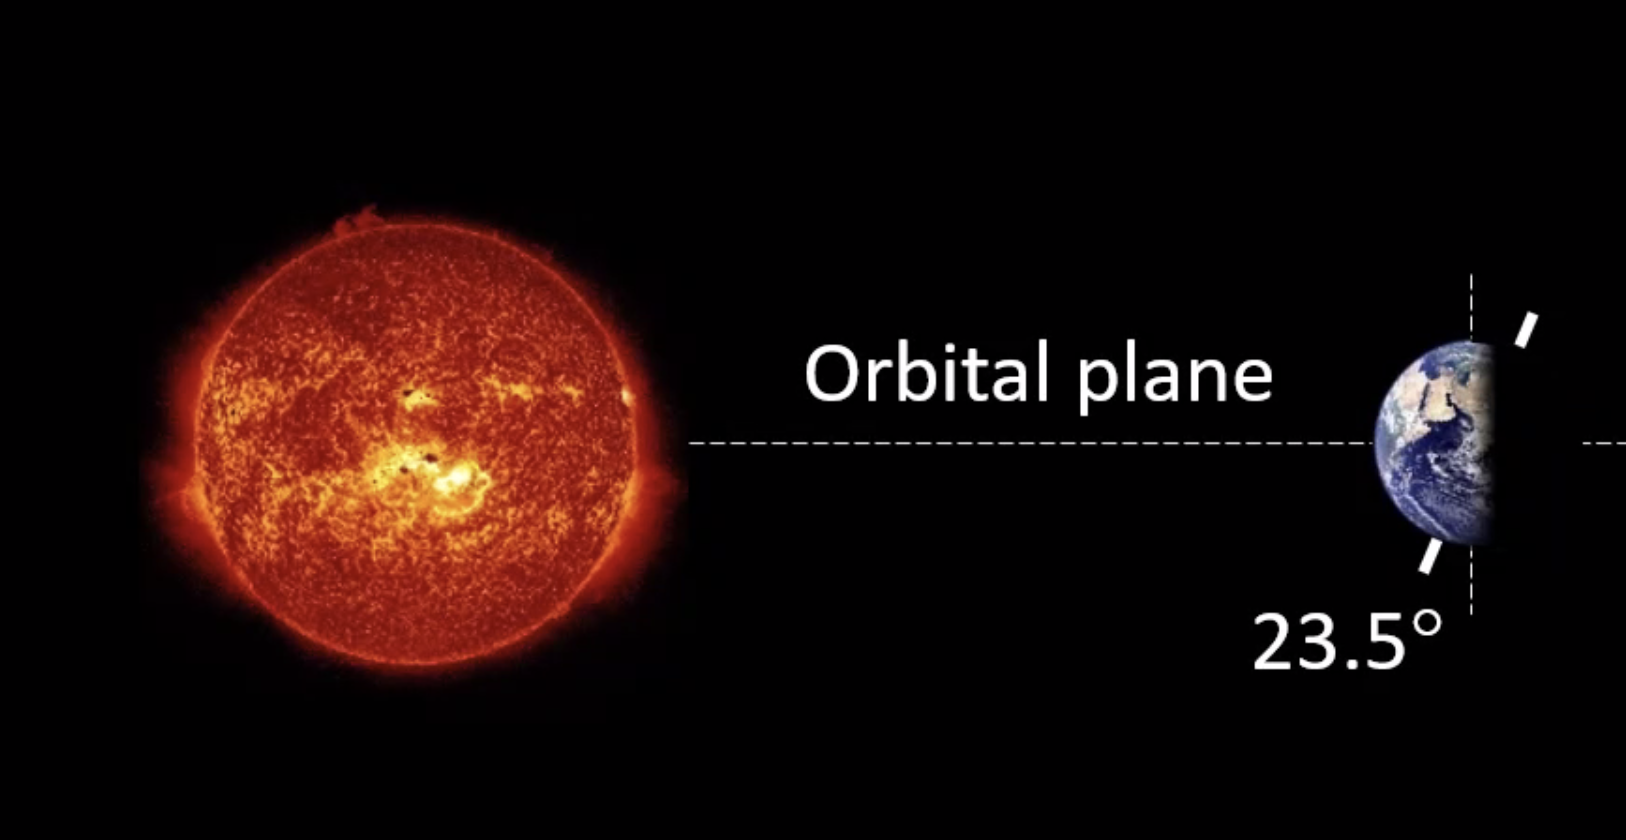
\includegraphics[width=0.5\linewidth]{content/img/axial_tilt.png}
    \caption{Current axial tilt is $23.5 \degree$}
\end{figure}

Earth's orbit is an ellipse. Sun is in one of its focal points.

\textbf{Perihelion} is when the Earth is the closest to the Sun, currently
153km (but changes depending on orbit's \textit{eccentricity}).

\textbf{Aphelion} is the furthest the Earth can be from the sun, currently
158km.

If axial tilt was $0 \degree$, there would be no seasons.

If axial tilt was $90 \degree$, there would be extreme seasonality.

%%%%%%%%%%%%%%%%%%%%%%%%%%%%%%%%%%%%%%%%%%%%%%%%%%%%%%%%%%%%%%%%%%%%%%%%%%%%%%%%
\textbf{Milankovic cycles}:

\begin{itemize}
    \item \textbf{axial tilt}: 41000 years cycle between $22.1 \degree$ and
    $24.5 \degree$
    \item \textbf{eccentricity}: 100000 and 413000 cycles, changes due to
    gravitational
    effect of other planets
    \item \textbf{precession} (wobble) of perihelion and aphelion along the
    orbit
\end{itemize}

\begin{figure}[H]
    \centering
    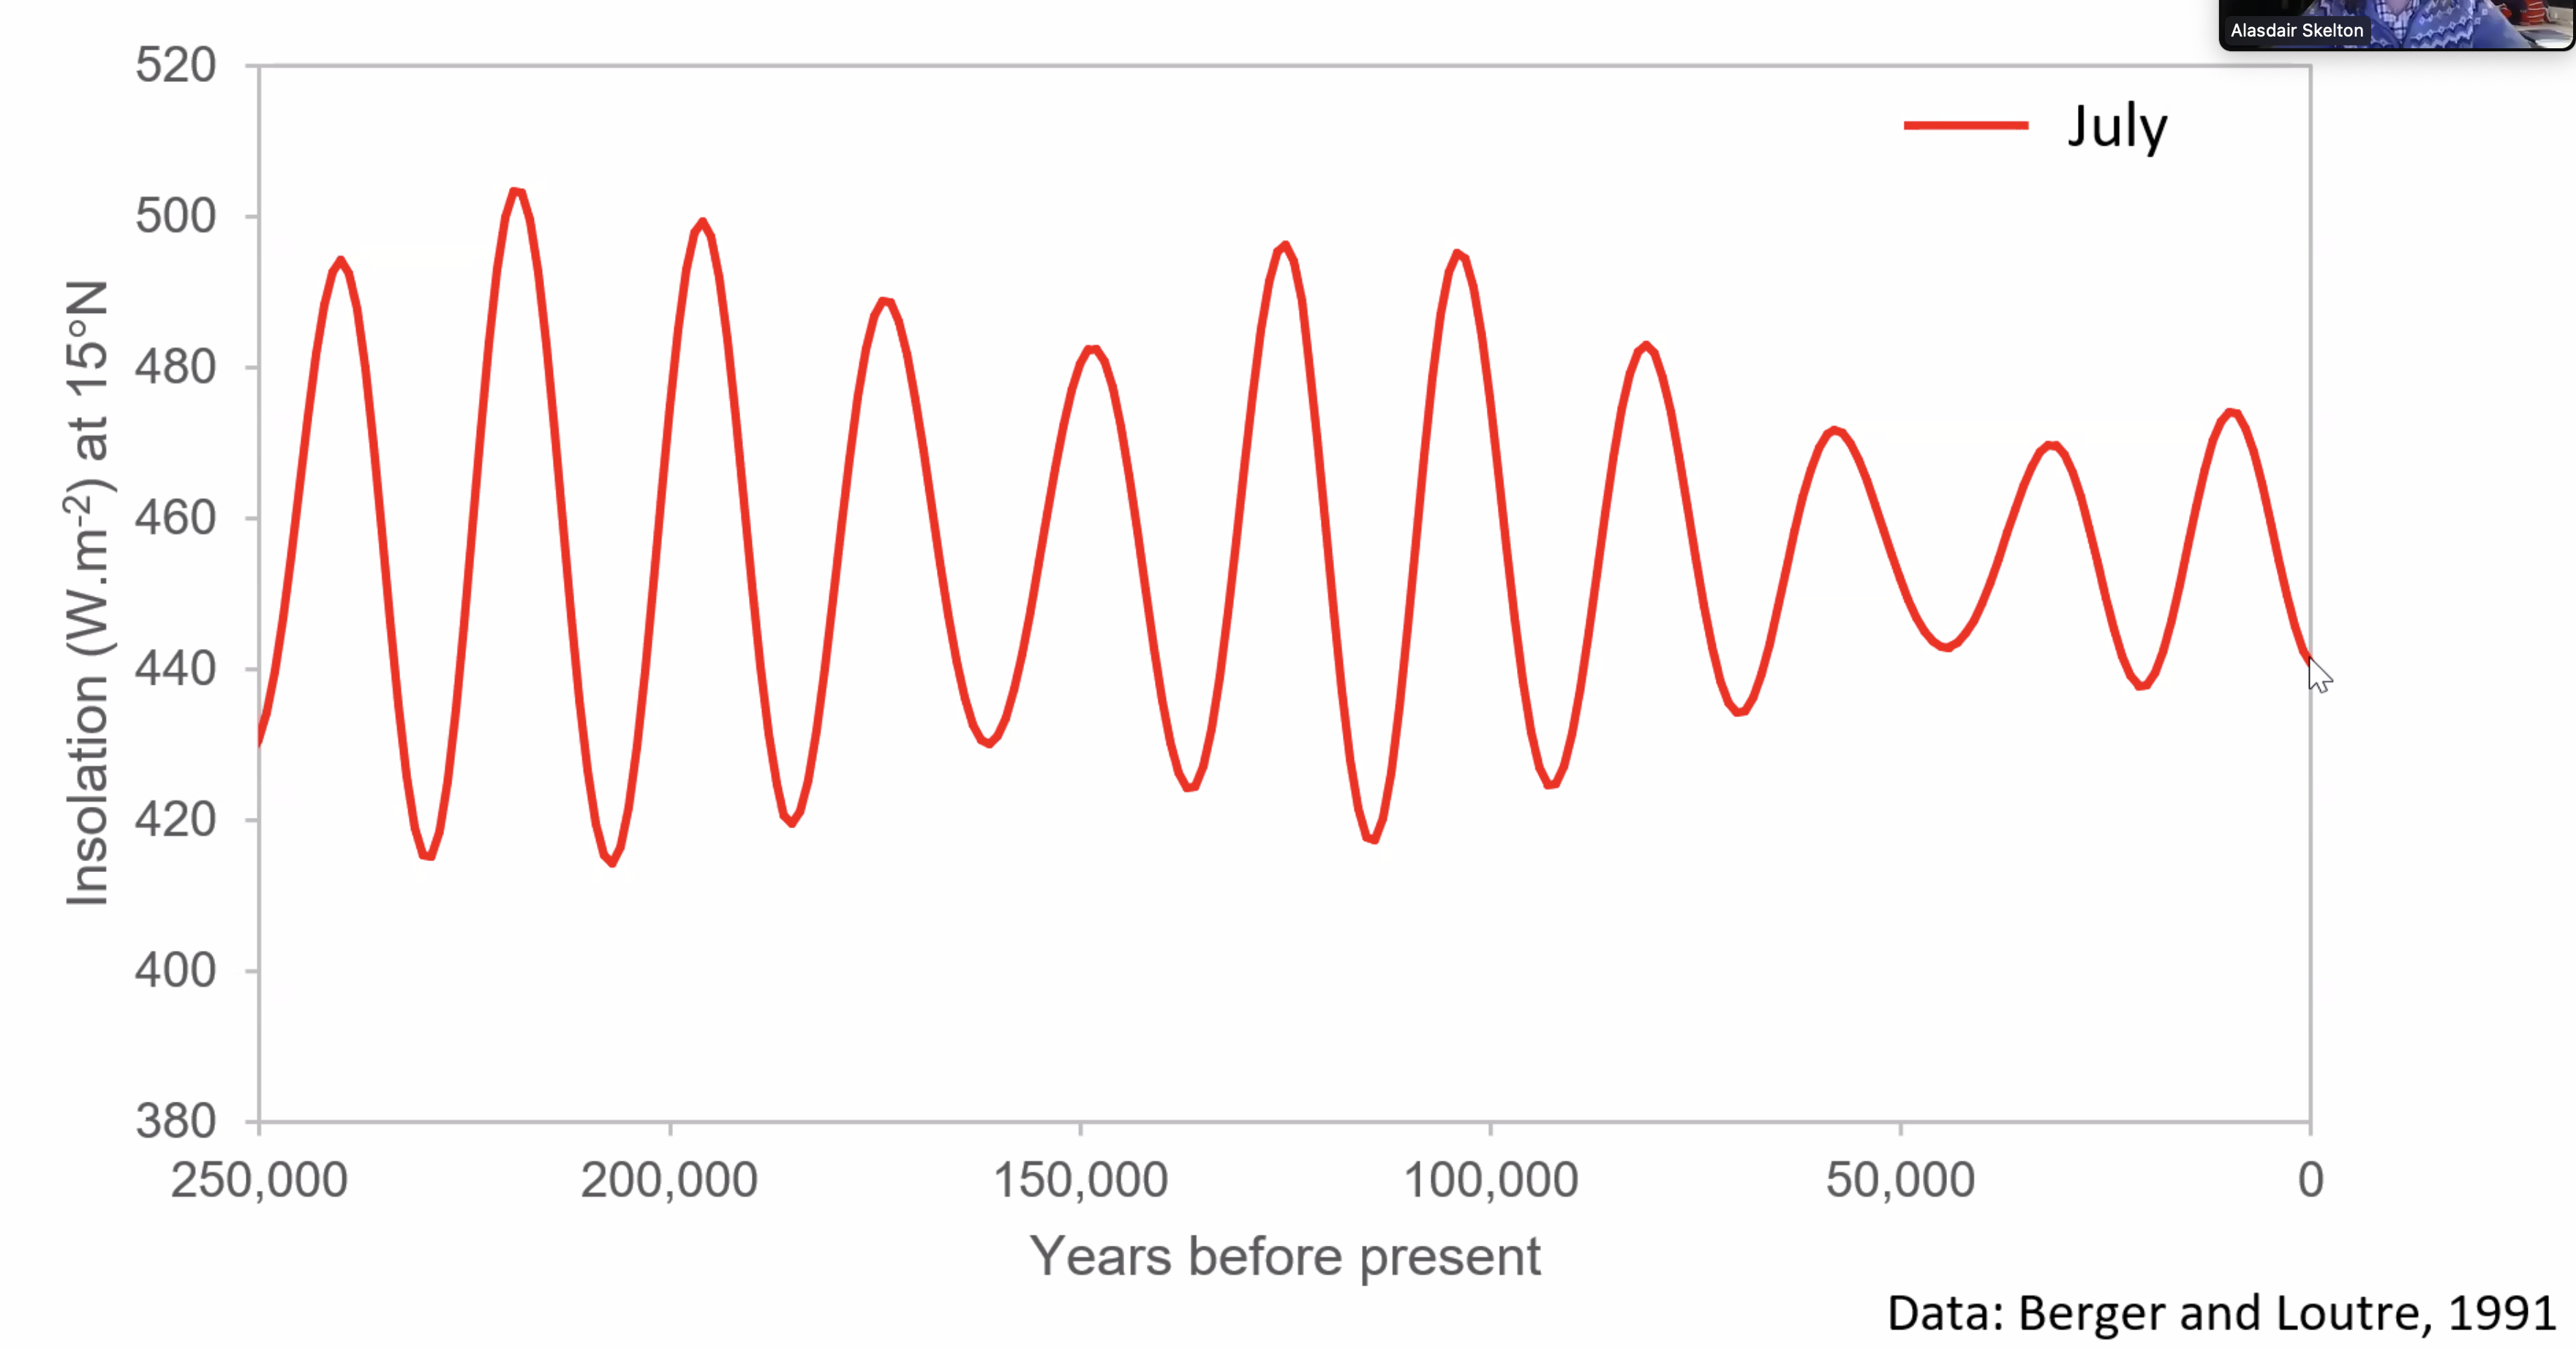
\includegraphics[width=1.0\linewidth]{content/img/insolation_in_july.png}
    \caption{Insolation in July}
\end{figure}

\begin{figure}[H]
    \centering
    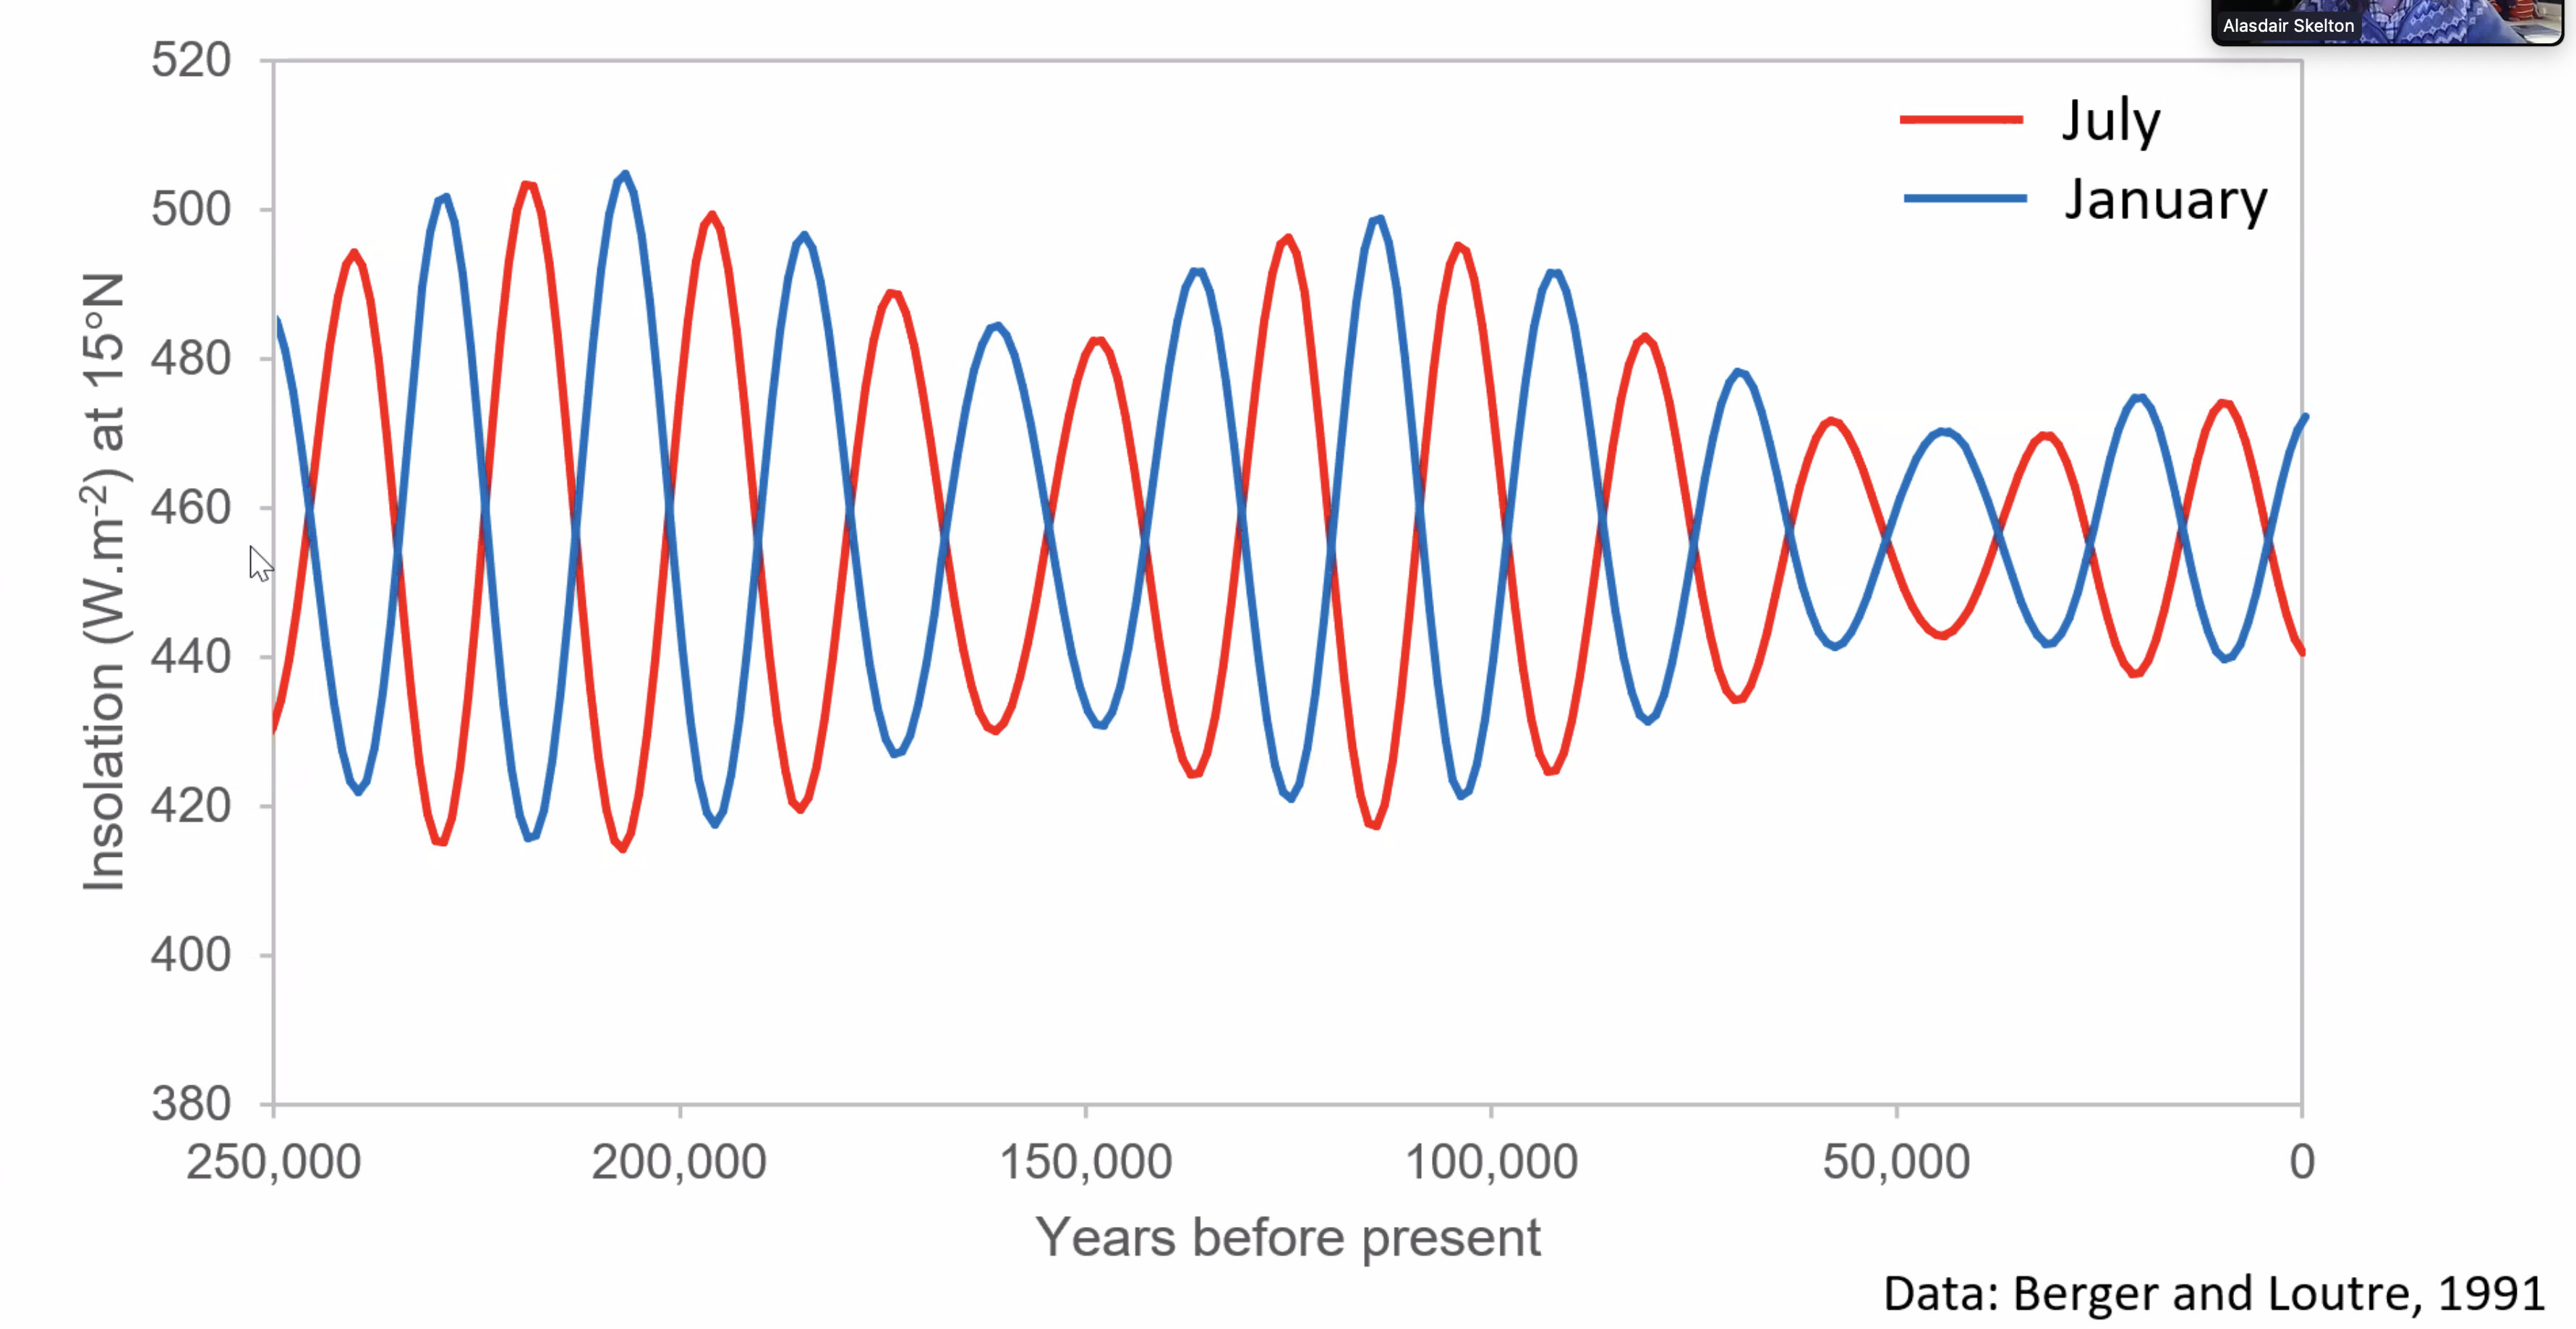
\includegraphics[width=1\linewidth]{content/img/insolation_july_january.png}
    \caption{Insolation in July and January}
\end{figure}

Milankovic cycles drive glaciations, not the other way around.

\subsection{Monsoons}

\begin{figure}[H]
    \centering
    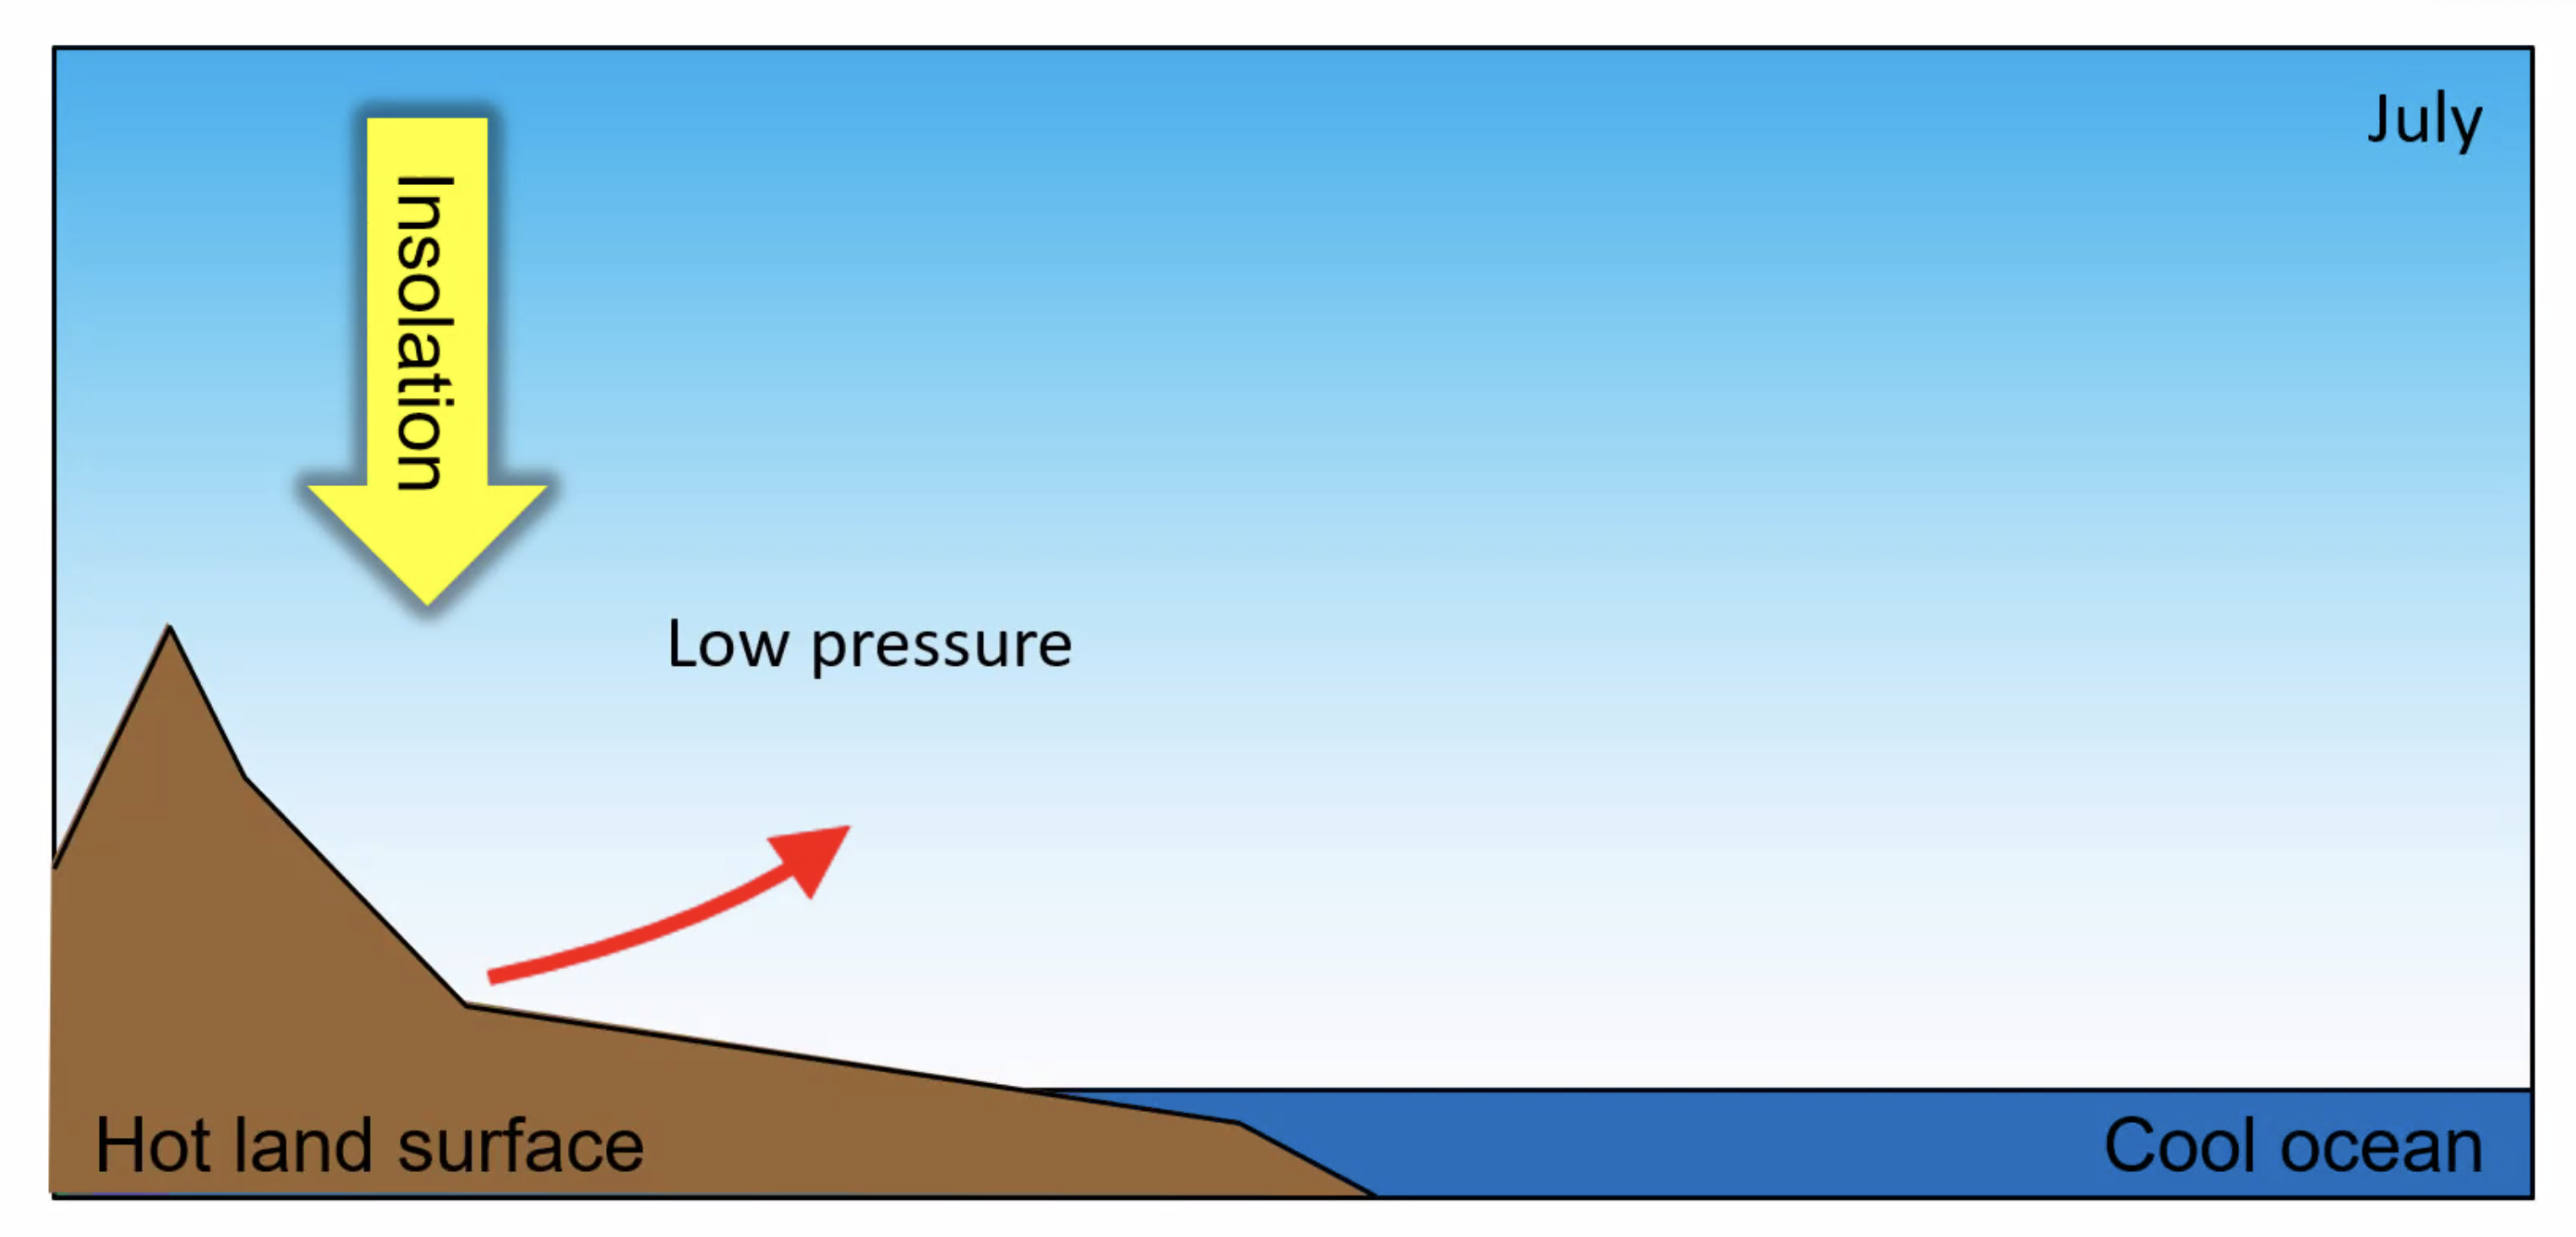
\includegraphics[width=0.5\linewidth]{content/img/monsoon_1.png}
    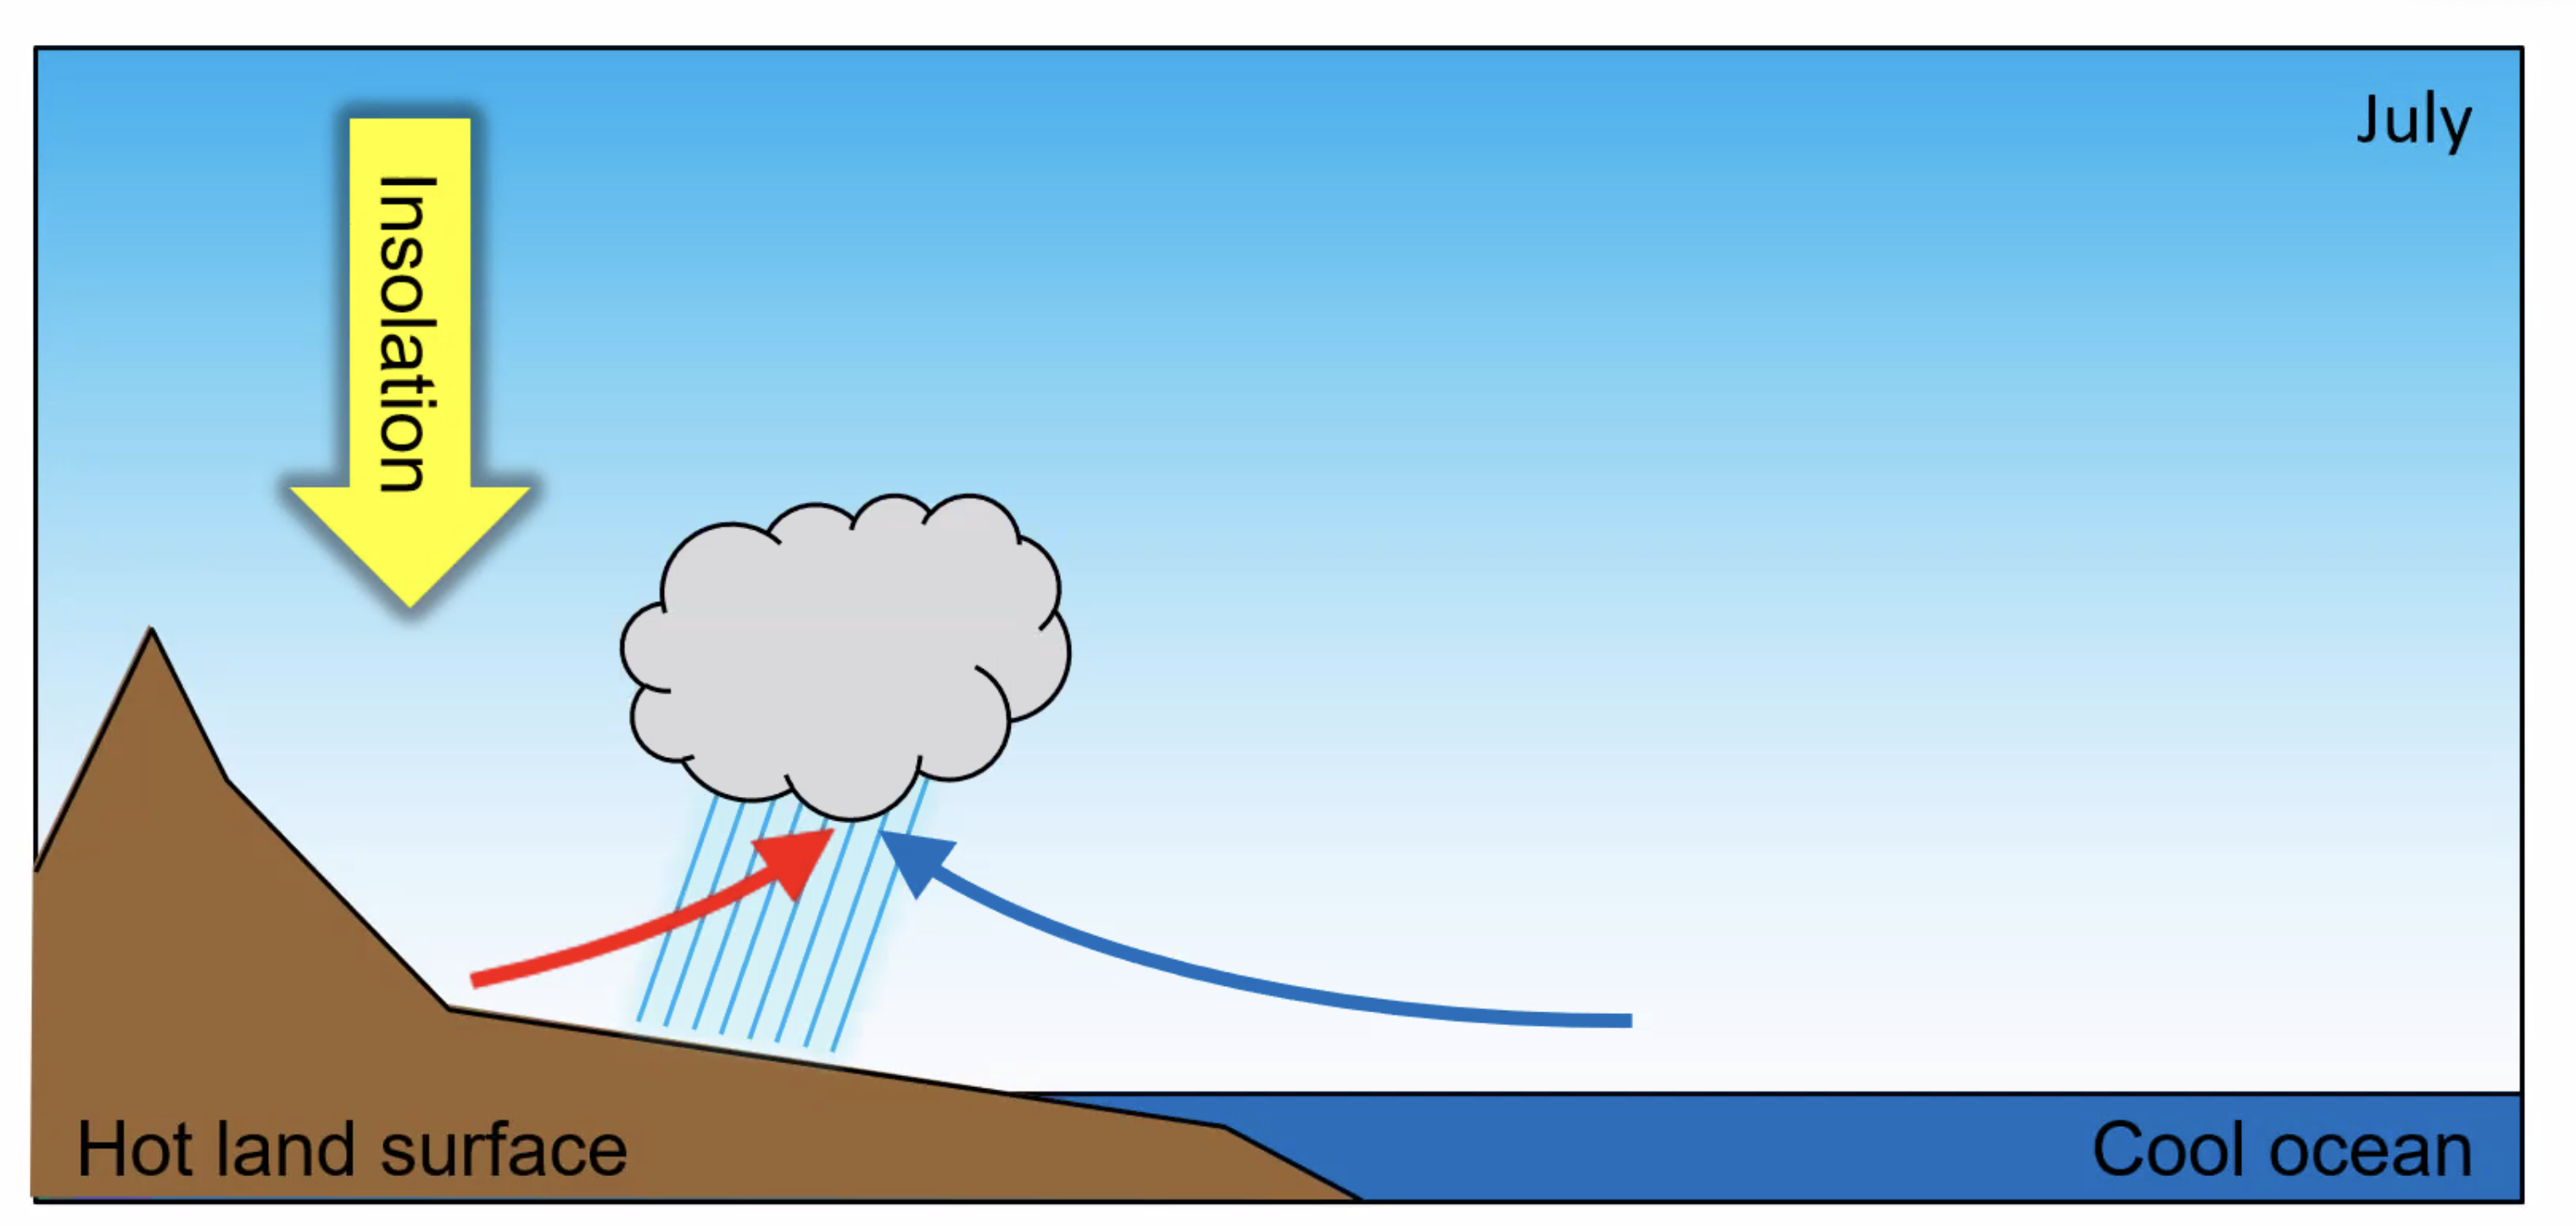
\includegraphics[width=0.5\linewidth]{content/img/monsoon_2.png}
    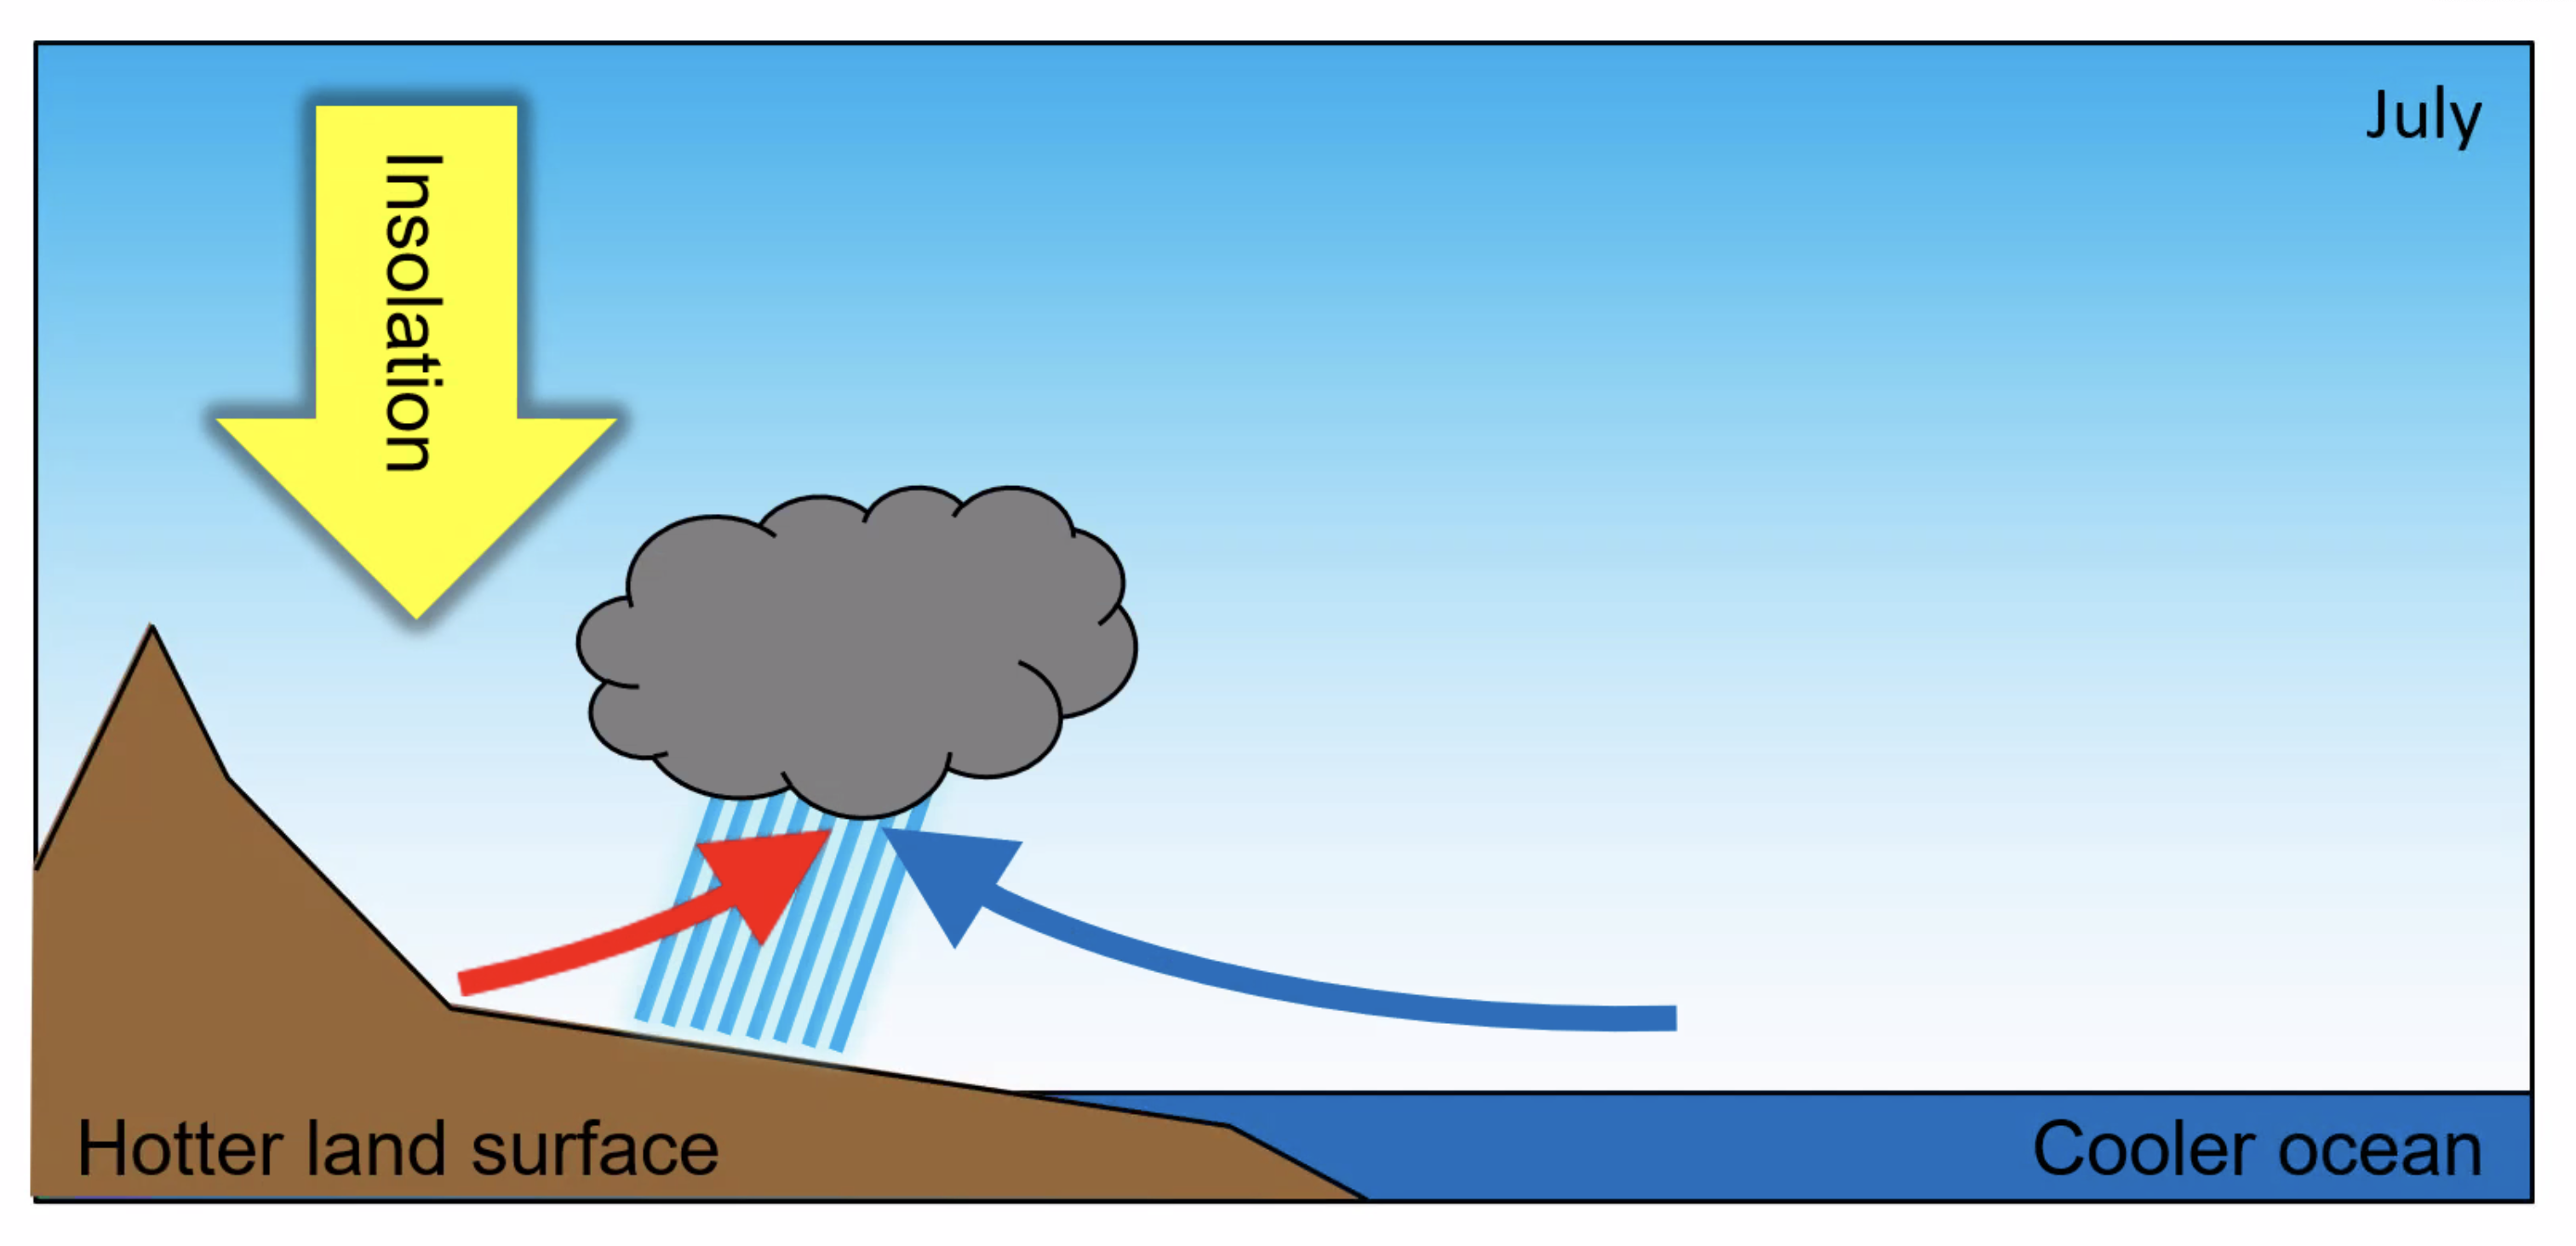
\includegraphics[width=0.5\linewidth]{content/img/monsoon_3.png}
    \caption{Summer monsoon}
\end{figure}

%%%%%%%%%%%%%%%%%%%%%%%%%%%%%%%%%%%%%%%%%%%%%%%%%%%%%%%%%%%%%%%%%%%%%%%%%%%%%%%%
\begin{figure}[H]
    \centering
    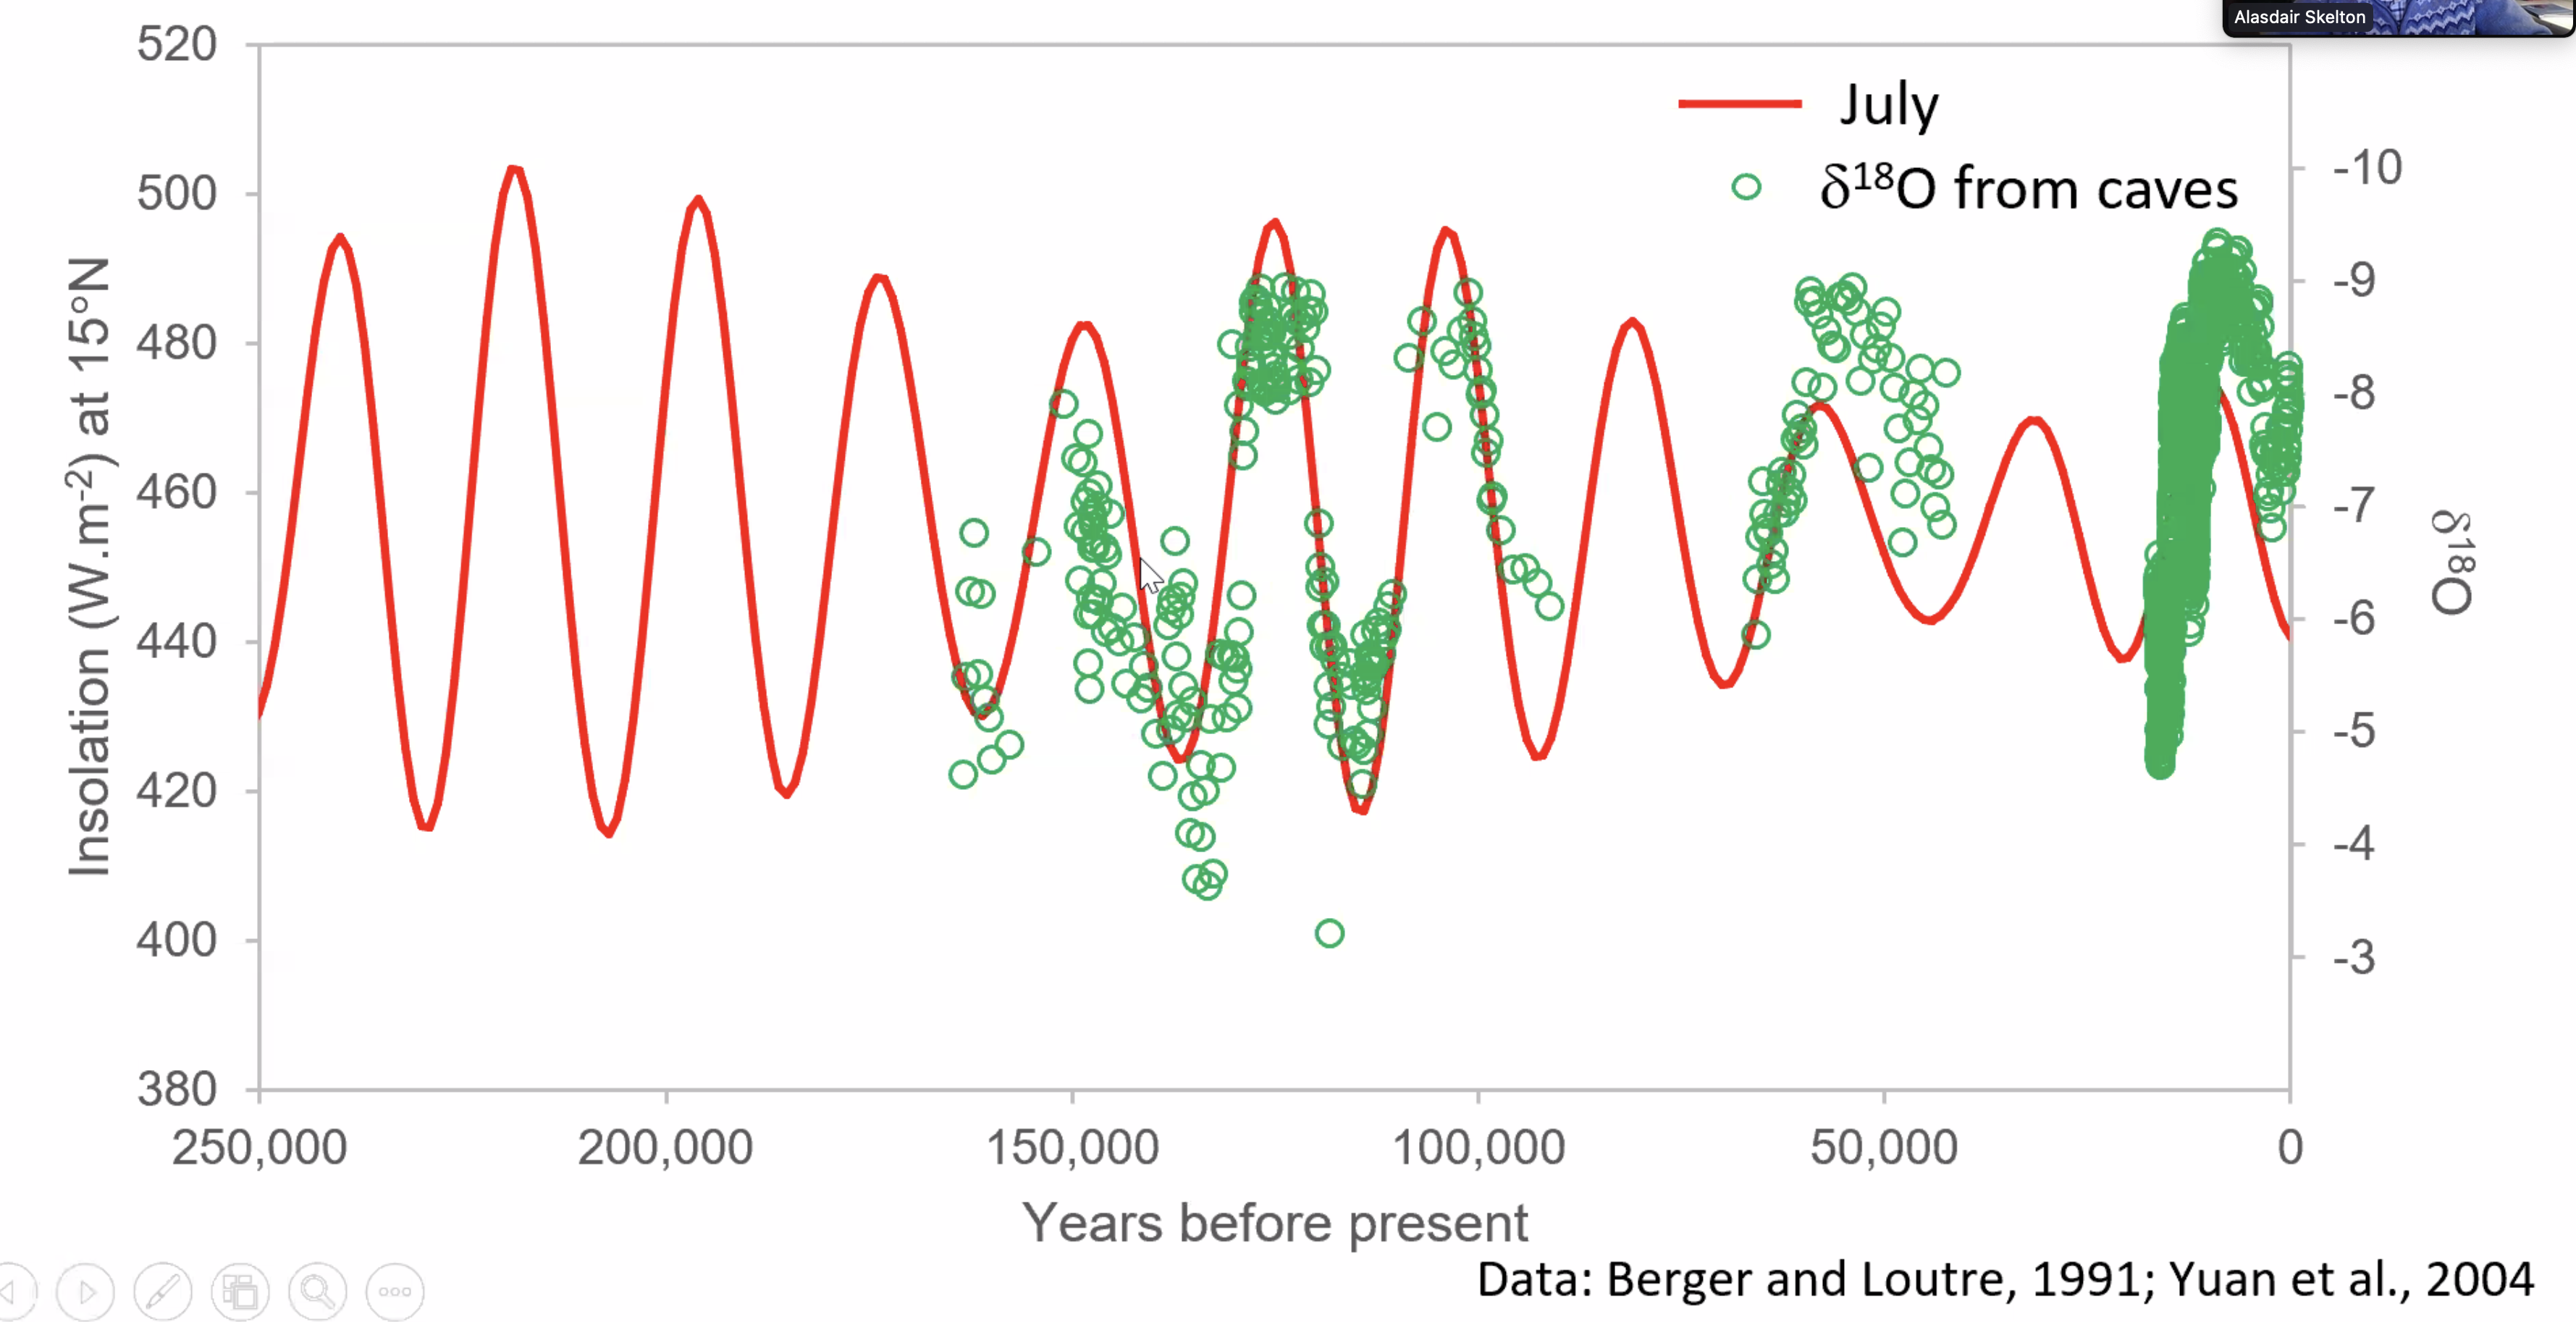
\includegraphics[width=0.75\linewidth]{content/img/monsoons_cave_proxy.png}
\end{figure}

\subsection{Glaciations}

\begin{figure}[H]
    \centering
    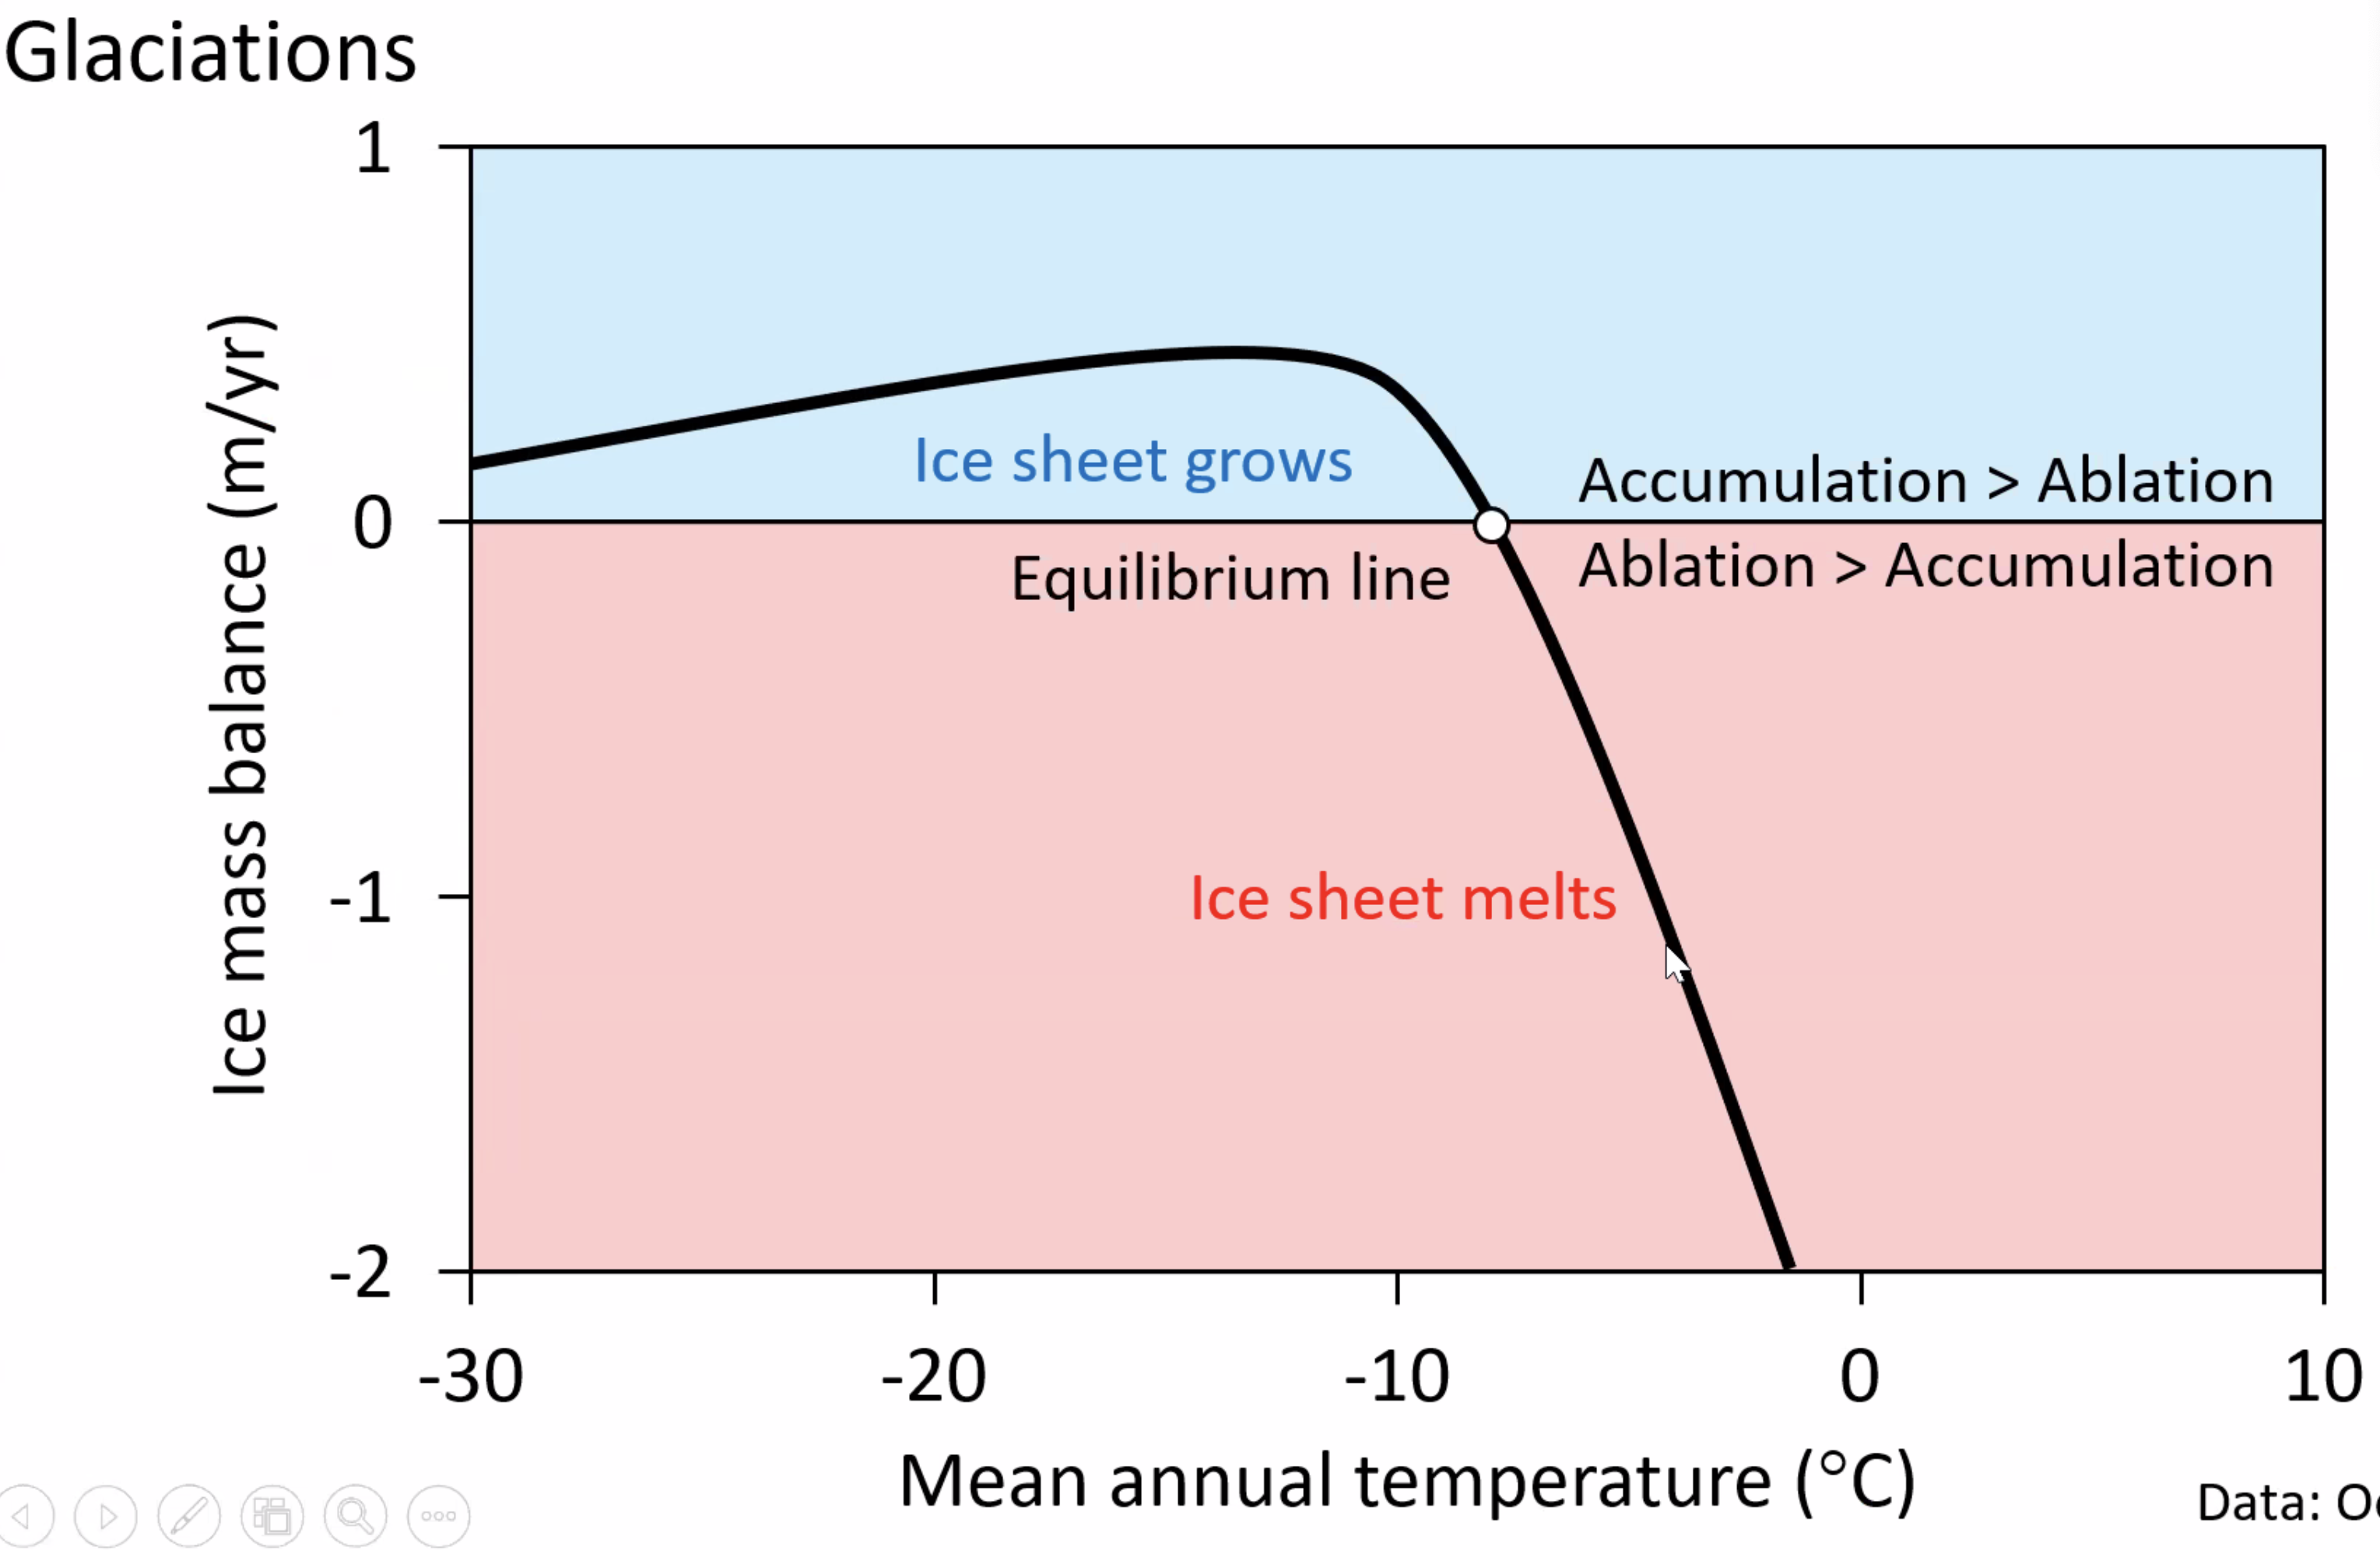
\includegraphics[width=0.75\linewidth]{
    content/img/ice_sheet_equilibrium.png}
\end{figure}

\begin{figure}[H]
    \centering
    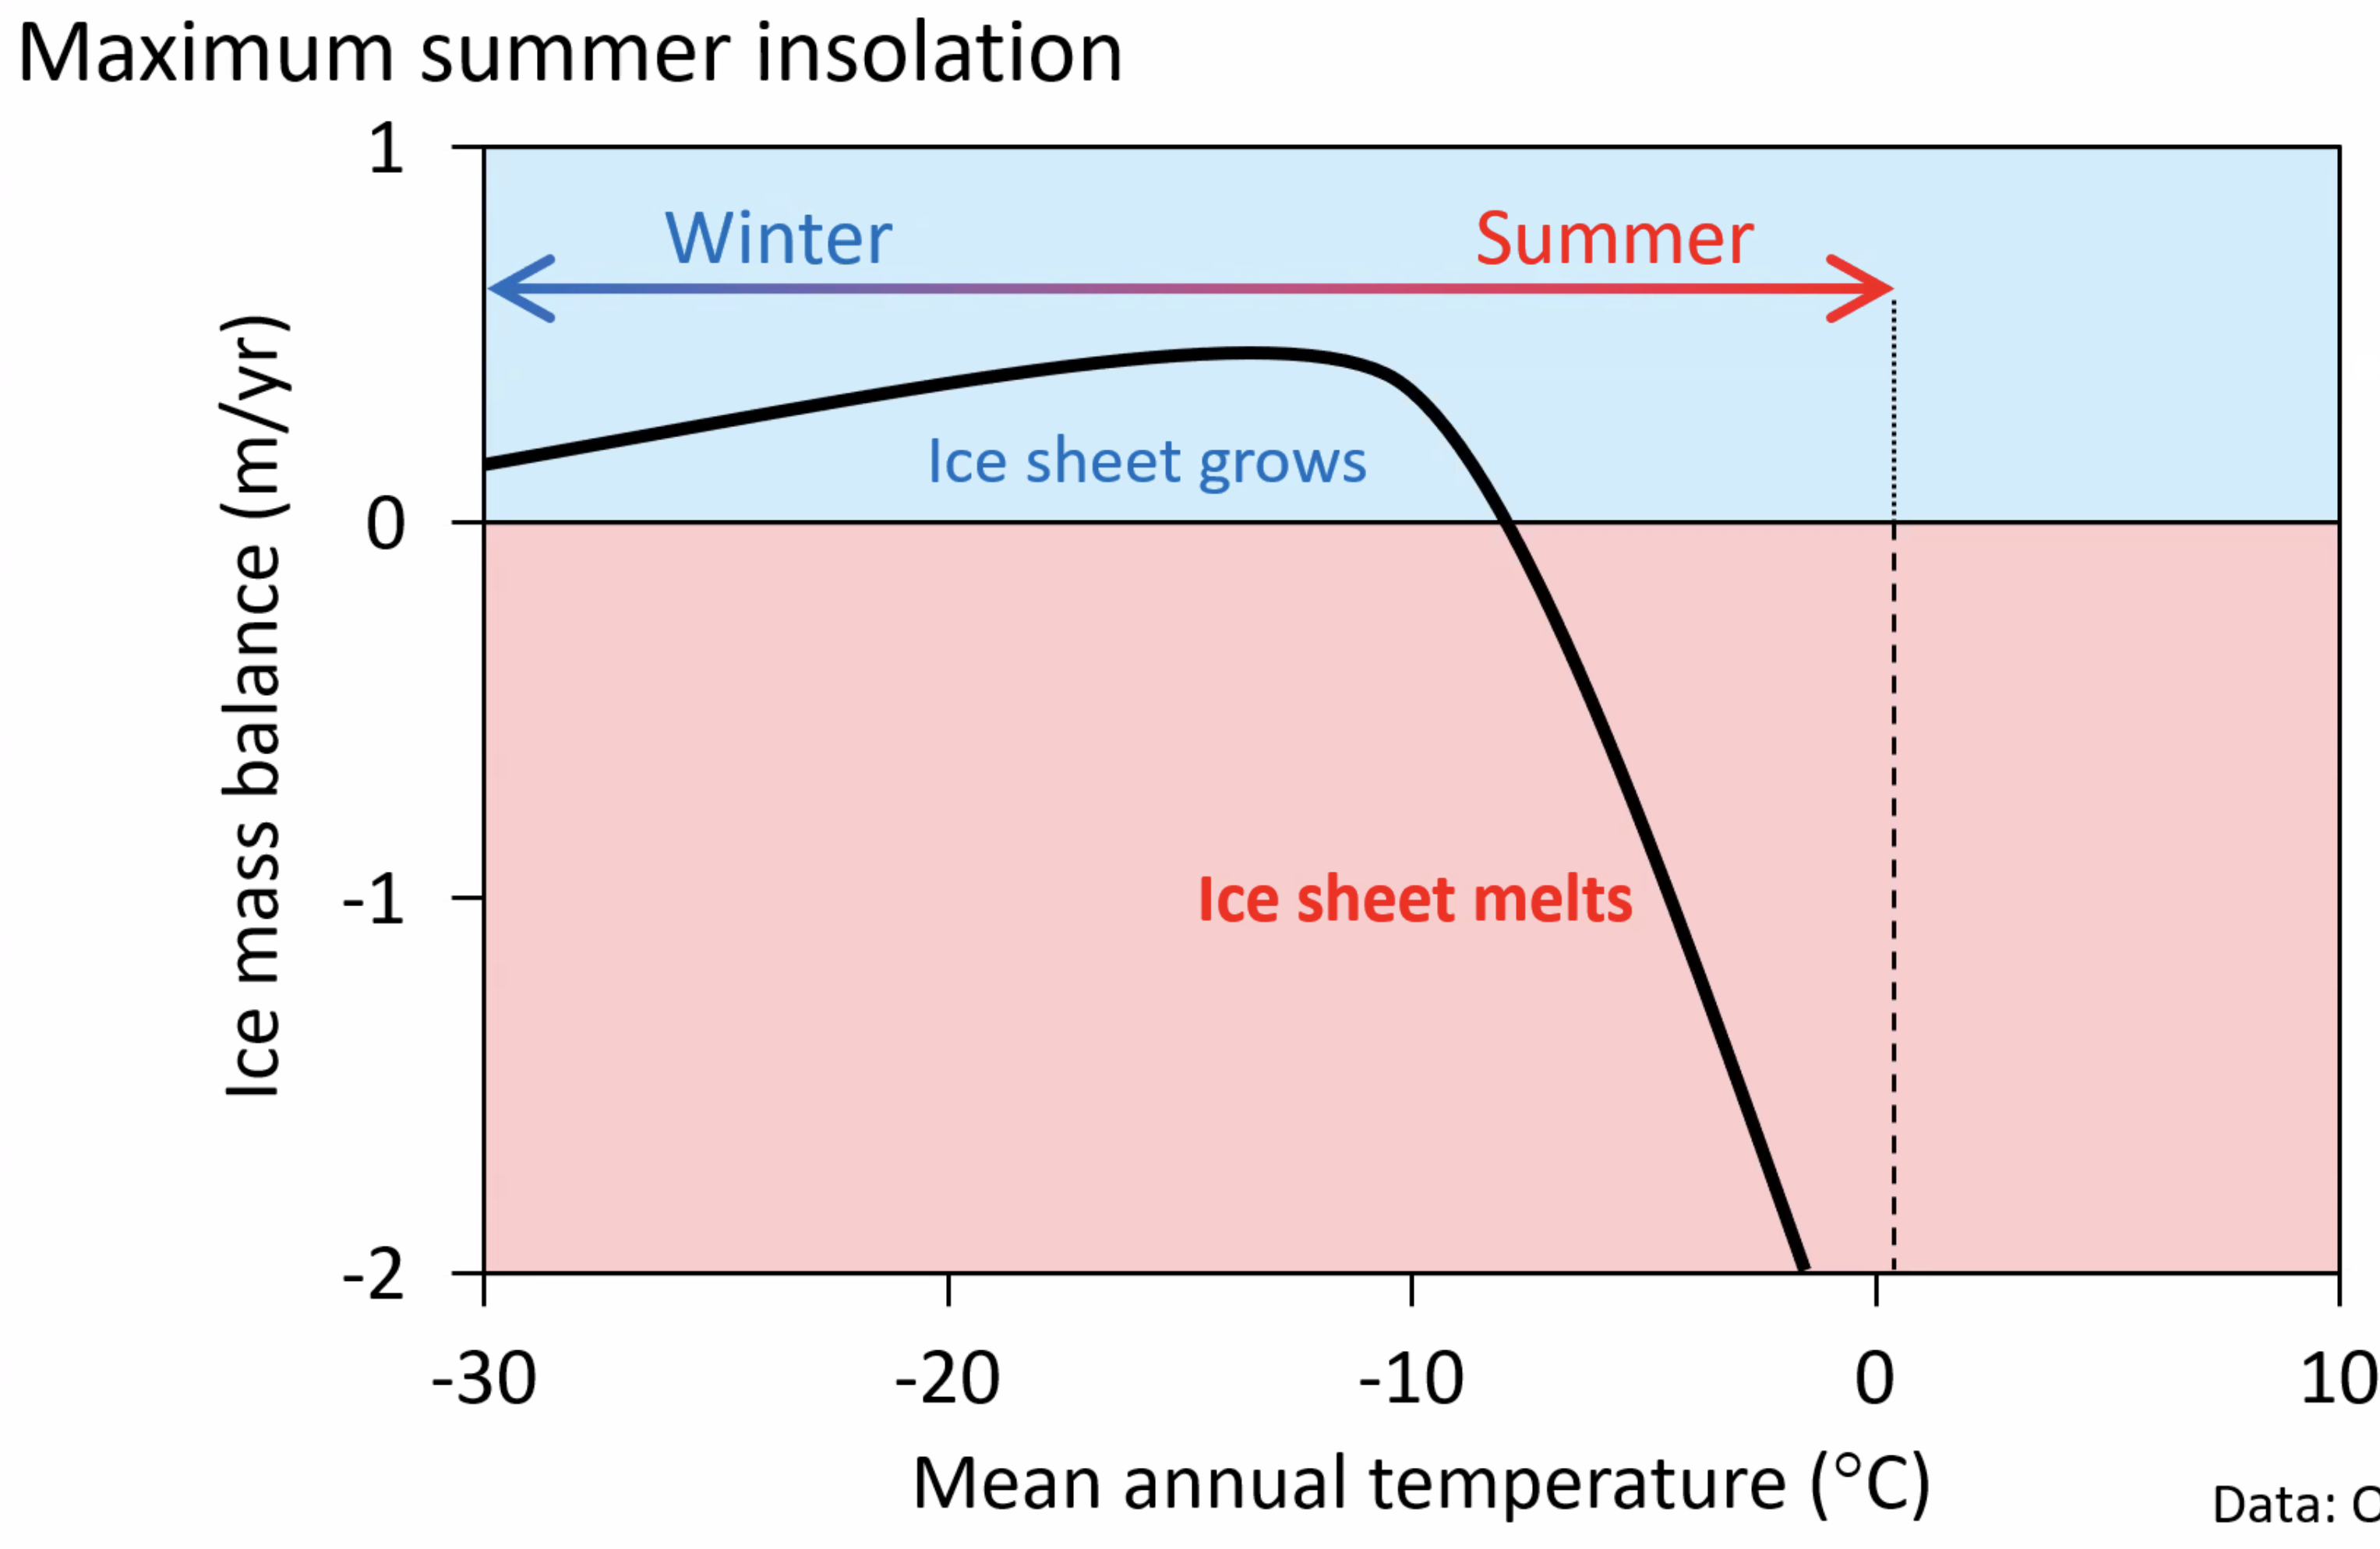
\includegraphics[width=0.75\linewidth]{
    content/img/maximum_summer_insolation.png}
    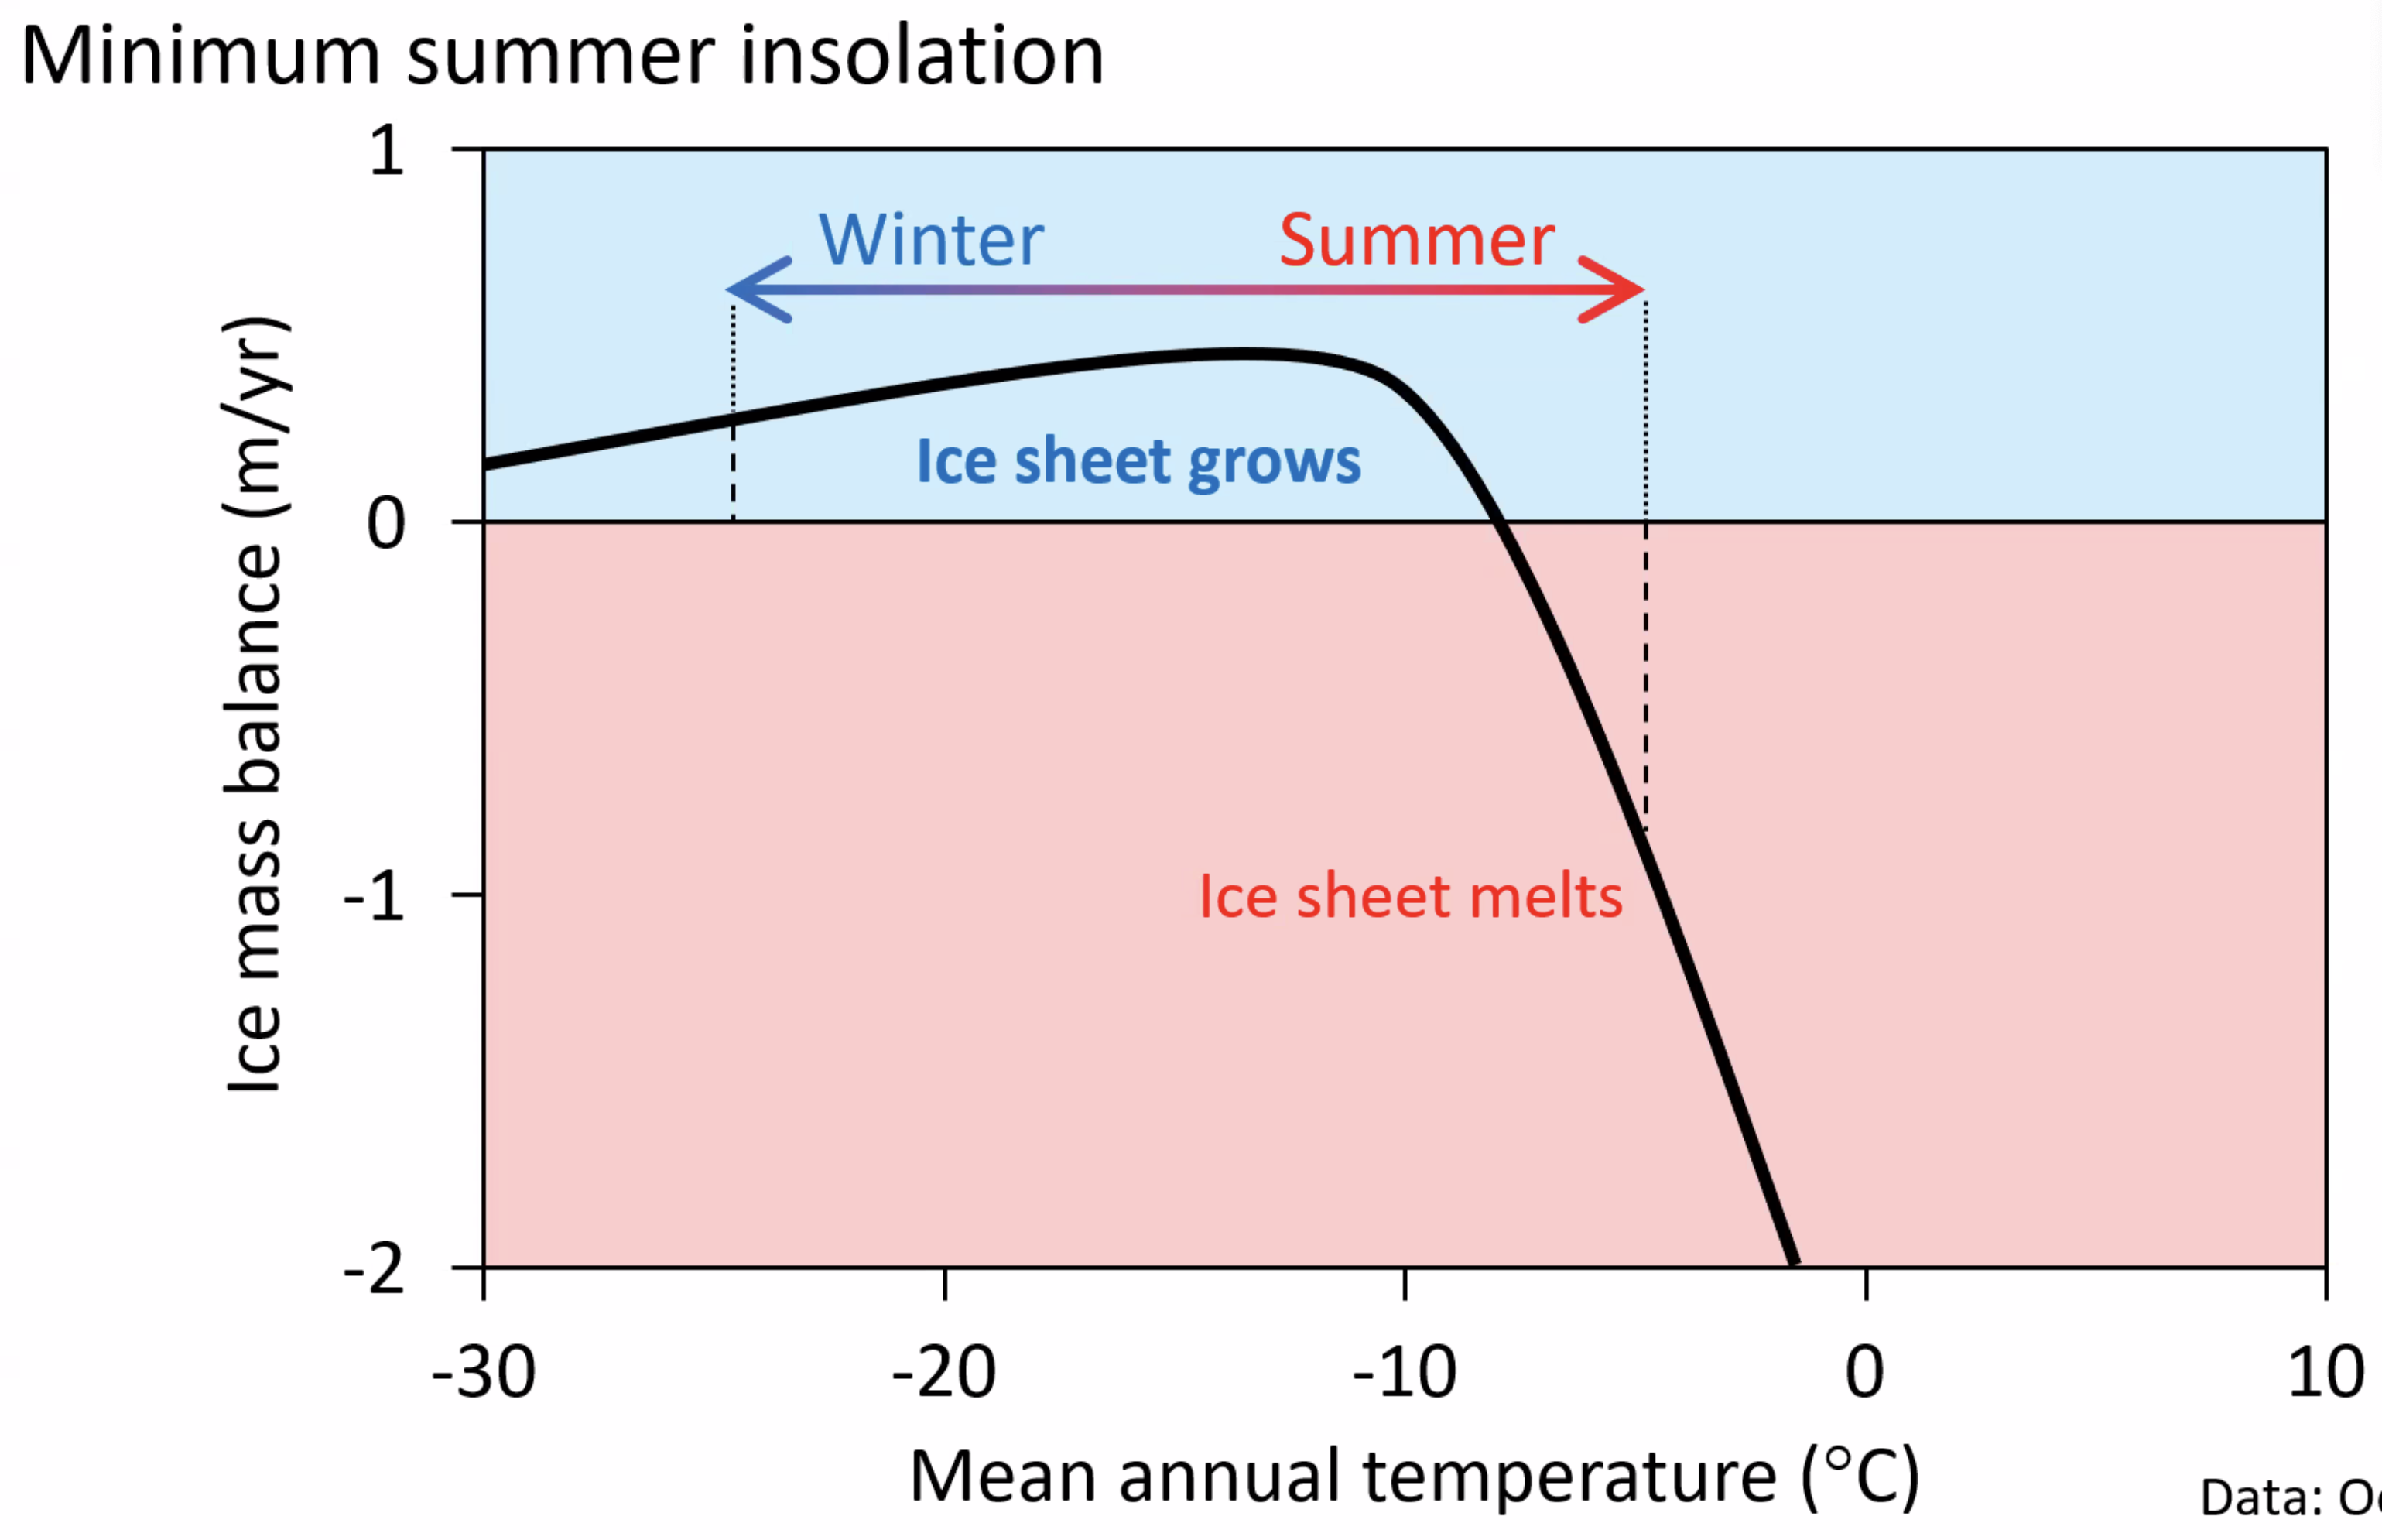
\includegraphics[width=0.75\linewidth]{
    content/img/minimum_summer_insolation.png}
\end{figure}

\begin{figure}[H]
    \centering
    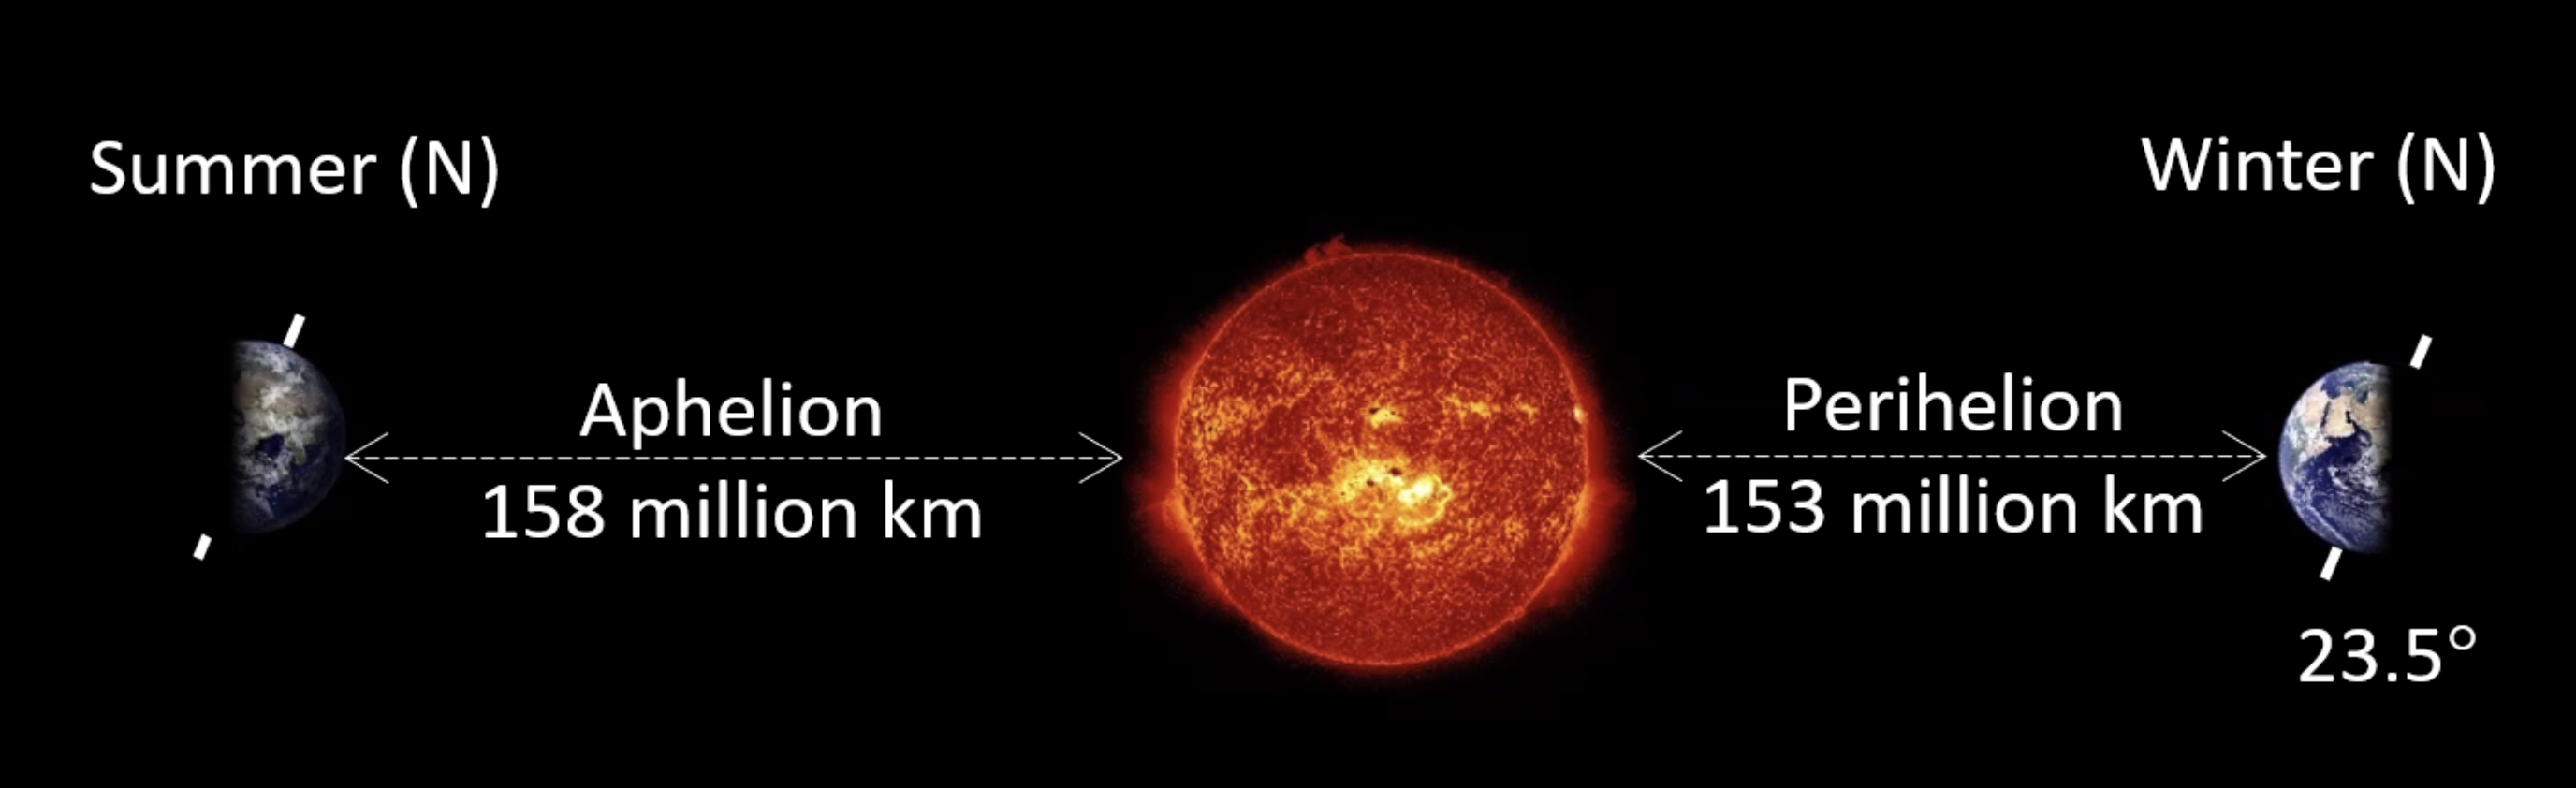
\includegraphics[width=0.75\linewidth]{
    content/img/aphelion_perihelion.png}
    \caption{Currently, axial tilt and eccentricity have opposite effects.
    Tilt is dominating which is why we are currently in interglacial.}
\end{figure}

\begin{figure}[H]
    \centering
    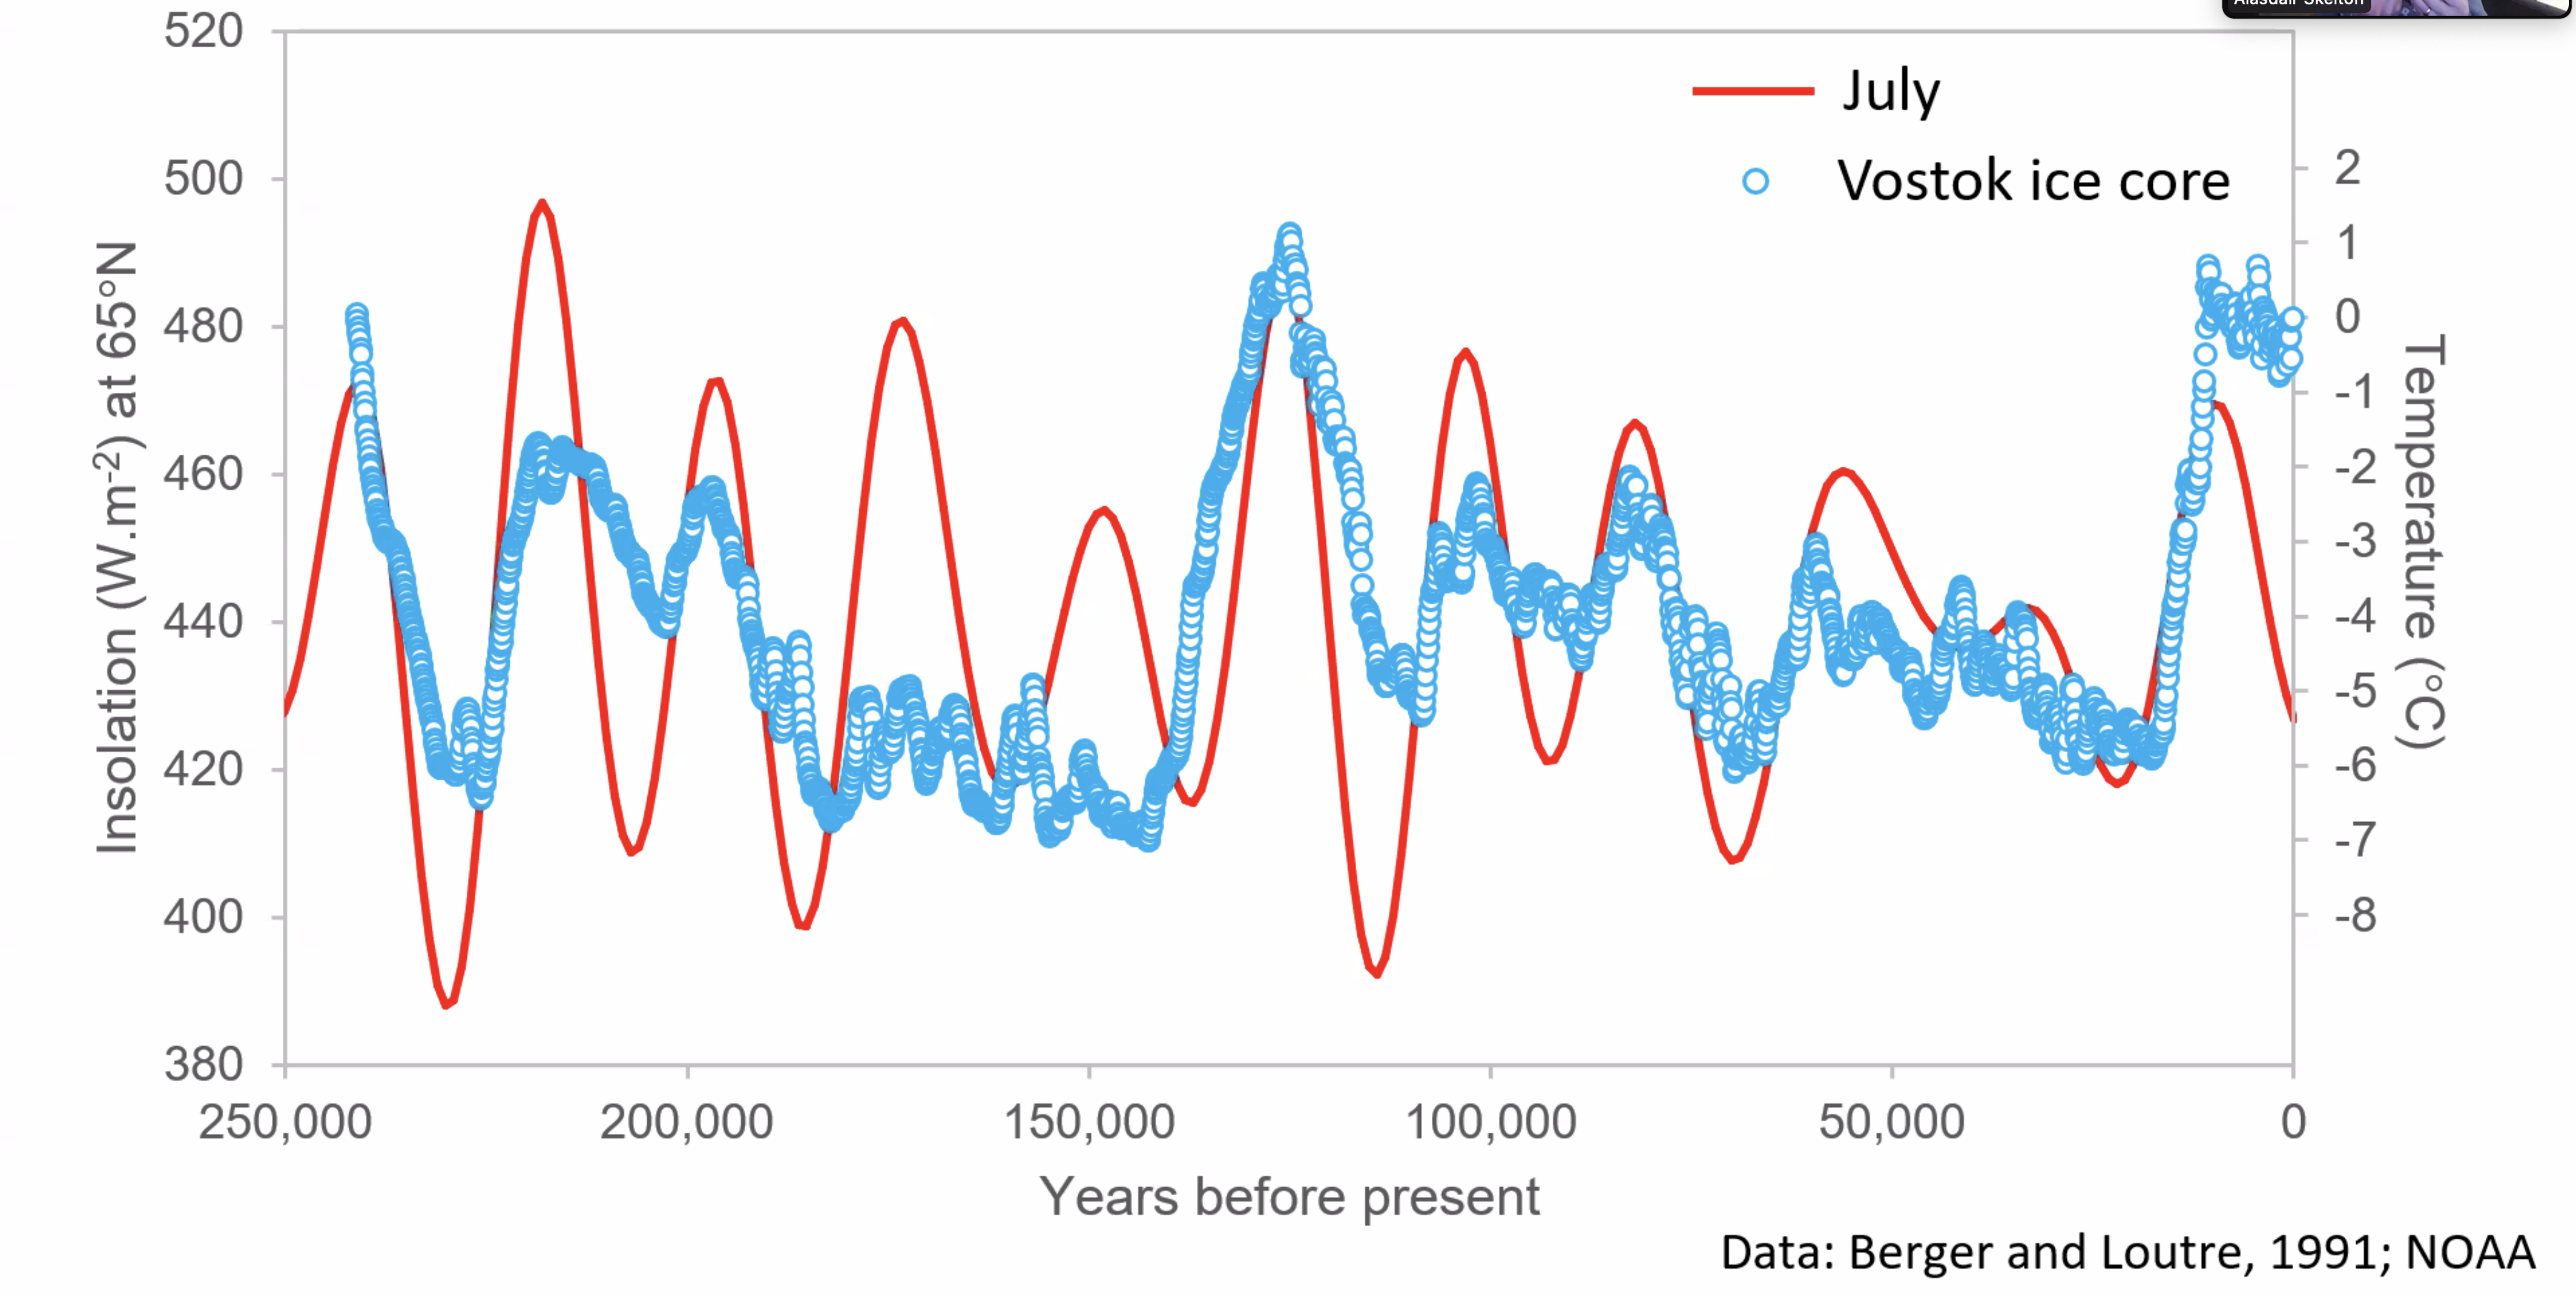
\includegraphics[width=0.75\linewidth]{content//img/vostok_ice_core.png}
\end{figure}

\section{Reading assignment 4: Plate Tectonics and Long-Term Climate}

In 1914 the German meteorologist Alfred Wegener proposed that continents move
slowly across Earth's surface. He was almost right: in fact \textit{all} of
Earth's surface slowly moves.

The best rocks to use as ancient compasses are basalts, which are rich in
highly magnetic iron. Basalts form the floors of ocean basins and are also
found on land in actively tectonic regions.

As the molten material cools, its iron-rich components align with Earth's
magnetic field like a compass. After lava turns into basaltic rock (when its
temperature drops below $1200 \degree$, continued cooling to temperatures near
$600 \degree$ allows the "fossilized" magnetic compases to become fixed in
position in the rock.

Also locked in the basalts are radioactive materials such as potassium (K)
which help date the basalt layers.

The age of the ocean crust steadily increases with distance from the ridges
(at divergent margins).

Since 450 Myr ago, major (continent-sized) ice sheets have existed on Earth
during three icehouse earas:
\begin{itemize}
	\item a brief interval centered near 445 Myr ago
	\item much longer interval from 325 to 240 Myr ago
	\item current icehouse era of the last 35 Myr
\end{itemize}

Most CO$_2$ is expelled to the atmosphere by volcanic activity at two kinds of
locations:

\begin{itemize}
	\item margins of converging plates, where parts of the subducting
	litosphere melt and form molten magmas that rise to the surface in
	mountain belt and island arc volcanoes, delivering CO$_2$ and other
	gases from Earth's interior
	\item where hot magma carrying CO$_2$ erupts directly into ocean water
\end{itemize}

\subsection{Key terms}

\textbf{continental crust}: the layer of igneous, metamorphic and sedimentary
rocks that forms the geological continents. It is 30-70 kilometers thick, has
an average composition like that of granite and is low in density
($2.7 \frac{g}{cm^3}$).

\textbf{ocean crust}: uppermost layer of the oceanic portion tectonic plates.
Average ocean floor is 4000 meters below sea level. Ocean crust is 5-10km
thick, has average composition like that of basalt and is higher in density
($3.2 \frac{g}{cm^3}$).

\textbf{mantle}: the layer of Earth that lies below both continental
and oceanic rust. It extends halfway towards the Earth's interior (2890km out
of 6370km). It is richer in heavy elements like iron (Fe) and magnesium (Mg).
It has dencity of $3.6 \frac{g}{cm^3}$).

\textbf{litosphere}: rock layer below Earth's surface. It is 100km thick and
generally behaves like hard, rigid substance. It enxompasses the crustal
layers and the upper part of the underlying mantle.

\textbf{asthenosphere}: the layer below litosphere, lying entirely within the
upper section of Earth's mantle at depths of 100 to 350 kilometers. It is
partly molten but mostly solid. It behaves like a soft, viscous fluid over long
intervals of time, and flows more easily.

\textbf{tectonic plates}: a division of the litosphere. These plates move at
rates ranging from <1 to 10 cm per year and average about the same rate as
growth of a fingernail.

\textbf{divergent margins}: one of 3 types of edges (margins) of tectonic
plates, occurring when plates move apart, for example in the middle of
Atlantic Ocean. This motion allows new ocean crust to be created. Plates
diverging at ocean ridges carry not just the near-surface layer of ocean crust
but also a much thicker layer of mantle lying underneath.

\textbf{convergent margins}: another type of edges (margins) of tectonic plates
occurring when plates come together.

\textbf{subduction}: a process occuring at convergent margins. The litosphere
(ocean crust and upper mantle) plunges deep into Earth's interio and ocean
trenches. For example, narrow mountain chains such as the Andes from on the
adjacent continnts because of the squeezing (compressing) forces produced when
the two plates move together.

\textbf{continental collision}: a less common type of converging plates. It
creates massive high-elevation regions such as the Tibetan Plateau.

\textbf{transform fault margins}: the last type of tectonic plates' edges, when
plates slide past each other. Sliding of plates at transform faults involves
the litosphere, both the upper continental crust and the underlying upper
mantle.

\textbf{magnetic field}: the Earth has a magnetic field that determines the
alignment of compass needles. Magnetic north is located a few degrees of
latitude away from geographic North Pole.

\textbf{paleomagnestism}: the study of prehistoric Earth's magnetic fields
recorded in rocks, sediments and archeological materials.

\textbf{magnetic lineations}: stripes of normal and reversed polarity records
growing symmetrically out of ocean ridges.

\textbf{seafloor spreading}: the process of divergence of litospheric plates
at ocean crust.

\textbf{polar position hypothesis} makes two predictions:
\begin{itemize}
	\item ice sheets should appear on continents that were located at
	polar or near-polar latitudes
	\item no ice should appear at times when continents were located
	outside of polar regions
\end{itemize}
In other words, it claims that land presence in polar region is both the
sufficient and necessary condition for glacier formation.

However, this hypothesis can be confirmed only one way: indeed polar
positioning of land is favorable to formation of glaciers, but it seems
not sufficient.

\textbf{Gondwana}: a large southern supercontinent consisting of modern
Africa, Arabia, Antarctica, Australia, South America and India. It was located
on the opposite side of the globe from North America, but it had begun a long
trip that would carry it across the South Pole.

\textbf{Pangaea}: the giant supercontinent, meaning "All Earth"

\textbf{evaporite}: deposits that precipitated out of water in lakes and
coatal margin basins with limited connections to the ocean. Evaporite salts
form only in arid regions where evaporation far exceeds precipitation.
More evaporite salt was deposited during the time of Pangaea than at any time
in the last several hundred million years.

\textbf{red beds}: sandy or silty sedimentary rocks stained various shades of
red by oxidation of iron minerals. Red-colored soils accumulate today in
regions where the contrast in seasonal moisture is strong.

\textbf{spreading rate hypothesis}: a hypothesis proposed in 1983 that the
climate changes during the last several hundred million years were driven
mainly by changes in the rate of CO$_2$ input to the atmosphere and ocean by
plate tectonic processes.

\textbf{hot spots}: volcanic hotspots are locales where thin plumes of molten
material rise from deep within the interior and reach the surface.

\textbf{uplift weathering hypothesis}: a proposition that chemical weathering
is an active driver of climate change, rather than just a passive negative
feedback that moderates climate. The hypothesis focuses on evidence that
exposure of fragmented and unweathered rock is a key factor in the intensity
of chemical weathering. It then links this evidence to the fact that freshly
fragmented rock is exposed mainly in regions of tectonic uplift.

\textbf{mass wasting}: erosional processes producing rock slides and falls,
flows of water-saturated debris, and a host of other processes that dislodge
everything from huge slabs of rock to loose boulders, pebbles and soil.

Uplift $\rightarrow$ (steep slopes, mass wasting, mountain glaciers, slope
precipitation) $\rightarrow$ increased rock fragmentation $\rightarrow$
increased weathering and CO$_2$ removal $\rightarrow$ global cooling

\subsection{Review questions}

\subsubsection{Does each litospheric plate correspond to an individual
continent or ocean basin?}
Most tectonic plates correspond to a combination of a continent and a part of
ocean basin.

\subsubsection{What kind of physical behaviour in Earth's deeper layers allows
the plates to move?}
Molten fluids circulating in Earth's liquid iron core create a magnetic field
analogous to that of a bar magnet.

\subsubsection{Explain how paleomagnetism tells us about past latitudes of
continents.}
The orientations of magnetic compases frozen in basalt layers deposited on
continents in relation to the magnetic poles are used. In molten lavas that
cool at high latitudes, the internal magnetic comasses point in a nearly
vertical direction because Earth's magnetic field has that orientation at high
latitudes. In contrast, lavas that cool near the equator have internal
compasses oriented closer to horizontal, nearly parallel to Earth's surface.

\subsubsection{Explain how paleomagnetism tells us about rates of spreading of
ocean ridges.}
Past changes in the magnetic field (inversed polarity) are recorded in fossil
magnetic compasses in well-dated basaltic rocks from many regions. These
changes are also recorded in magnetic lineations -- stripes of normal and
reversed polarity recorded in ocean crust -- growing symmetrically out of ocean
ridges.

\subsubsection{Do glaciations \textit{always} occur when continents are located
in polar positions?}
No, there were greenhouse eras (no glaciations) with continents in polar
regions.

\subsubsection{What are the major characteristics of the climate of Pangaea?}
No ice sheets existed even though its norther and southern limits ay within
Arctic and Antarctic circles. This suggests that Pangaea's climate was
somewhat warmer than today's climate. This is also supported by fossil evidence
of vegetation. Several kinds of palm-like vegetation that would have been
killed by hard freezes existed on Pangaea to latitudes as high as $40 \degree$.
Because the moderating effcts of ocean moisture failed to reach much of
Pangaea's interior, the continent was left vulnerable to seasonal extremes of
solar heating in summer and cooling during winter.

\subsubsection{What is the central concept behind the BLAG (spreading rate)
hypothesis?}
That changes in the average rate of seafloor spreading over millions of years
have controlled the rate of delivery of CO$_2$ to the atmosphere from the
large subsurface rock reservoir of carbon and that the resulting changes in
atmospheric CO$_2$ concentrations have had an impact on Earth's climate.

\subsubsection{What role does chemical weathering play in the BLAG hypothesis?}
It creates a negative feedback. Warmer climate leads to more precipitation,
thus more vegetation, thus higher removal of CO$_2$ from the atmosphere.

\subsubsection{Write a chemical reaction showing how weathering removes
CO$_2$ from the atmosphere.}
$\underset{\text{Silicate rock}}{\text{CaSiO}_2} +
\underset{\text{Atmosphere}}{\text{CO}_2}
\rightarrow
\underset{\text{Plankton}}{\text{CaCO}_3}
+
\underset{\text{Plankton}}{\text{SiO}_2}$

\subsubsection{How soon after deposition does freshly fragmented debris undergo
most chemical weathering?}

\subsubsection{Why is chemical weathering faster in the eastern Andes than in
the Amazon lowlands?}
The minerals in Amazon lowlands have long been "used up" in the weathering
process, while the physical impacts of active uplift in the Andes (steep
slopes, earthquakes, mass wasting, heavy precipitation, and glacial erosion)
combine to generate a continual supply of fresh, finely ground rock debris for
weathering.

\subsubsection{How could chemical weathering be both the driver and the
thermostat of Earth's climate?}
The effects of the uplift weathering processes are probably opposed by the
chemical weathering thermostat.

\subsubsection{Fast subduction in the modern Pacific Ocean carries down
sediments with low amounts of CaCO$_3$ while almost no subduction occurs in
the Atlantic Ocean, with its carbonate-rich sediments. What would happen if
subduction suddenly began in the Atlantic and replaced an equal amount of
subduction in the Pacific?}

%%%%%%%%%%%%%%%%%%%%%%%%%%%%%%%%%%%%%%%%%%%%%%%%%%%%%%%%%%%%%%%%%%%%%%%%%%%%%%%%
\section{Lecture 4: Climate variability on a timescale of millions of years}

\subsection{Theory of plate tectonics}

\subsubsection{Alfred Wegener's hypothesis of continental drift}

\textbf{Glossopteris}: Example of a tree which is found fossilized (leaves)
on multiple continents.

\textbf{Caledonides}
The mountain chain in Scandinavia was once joined with Caledonides in
North-East America and North-West Africa. It was one mountain belt when all
continents were together.

\subsection{Patrick Blackett's polar wander}

If you look at volcanic rocks, as they solidify, they contain certain magnetic
minerals and they line up in magma as they crystallize, and they point towards
the North Pole.

\begin{figure}[H]
    \centering
    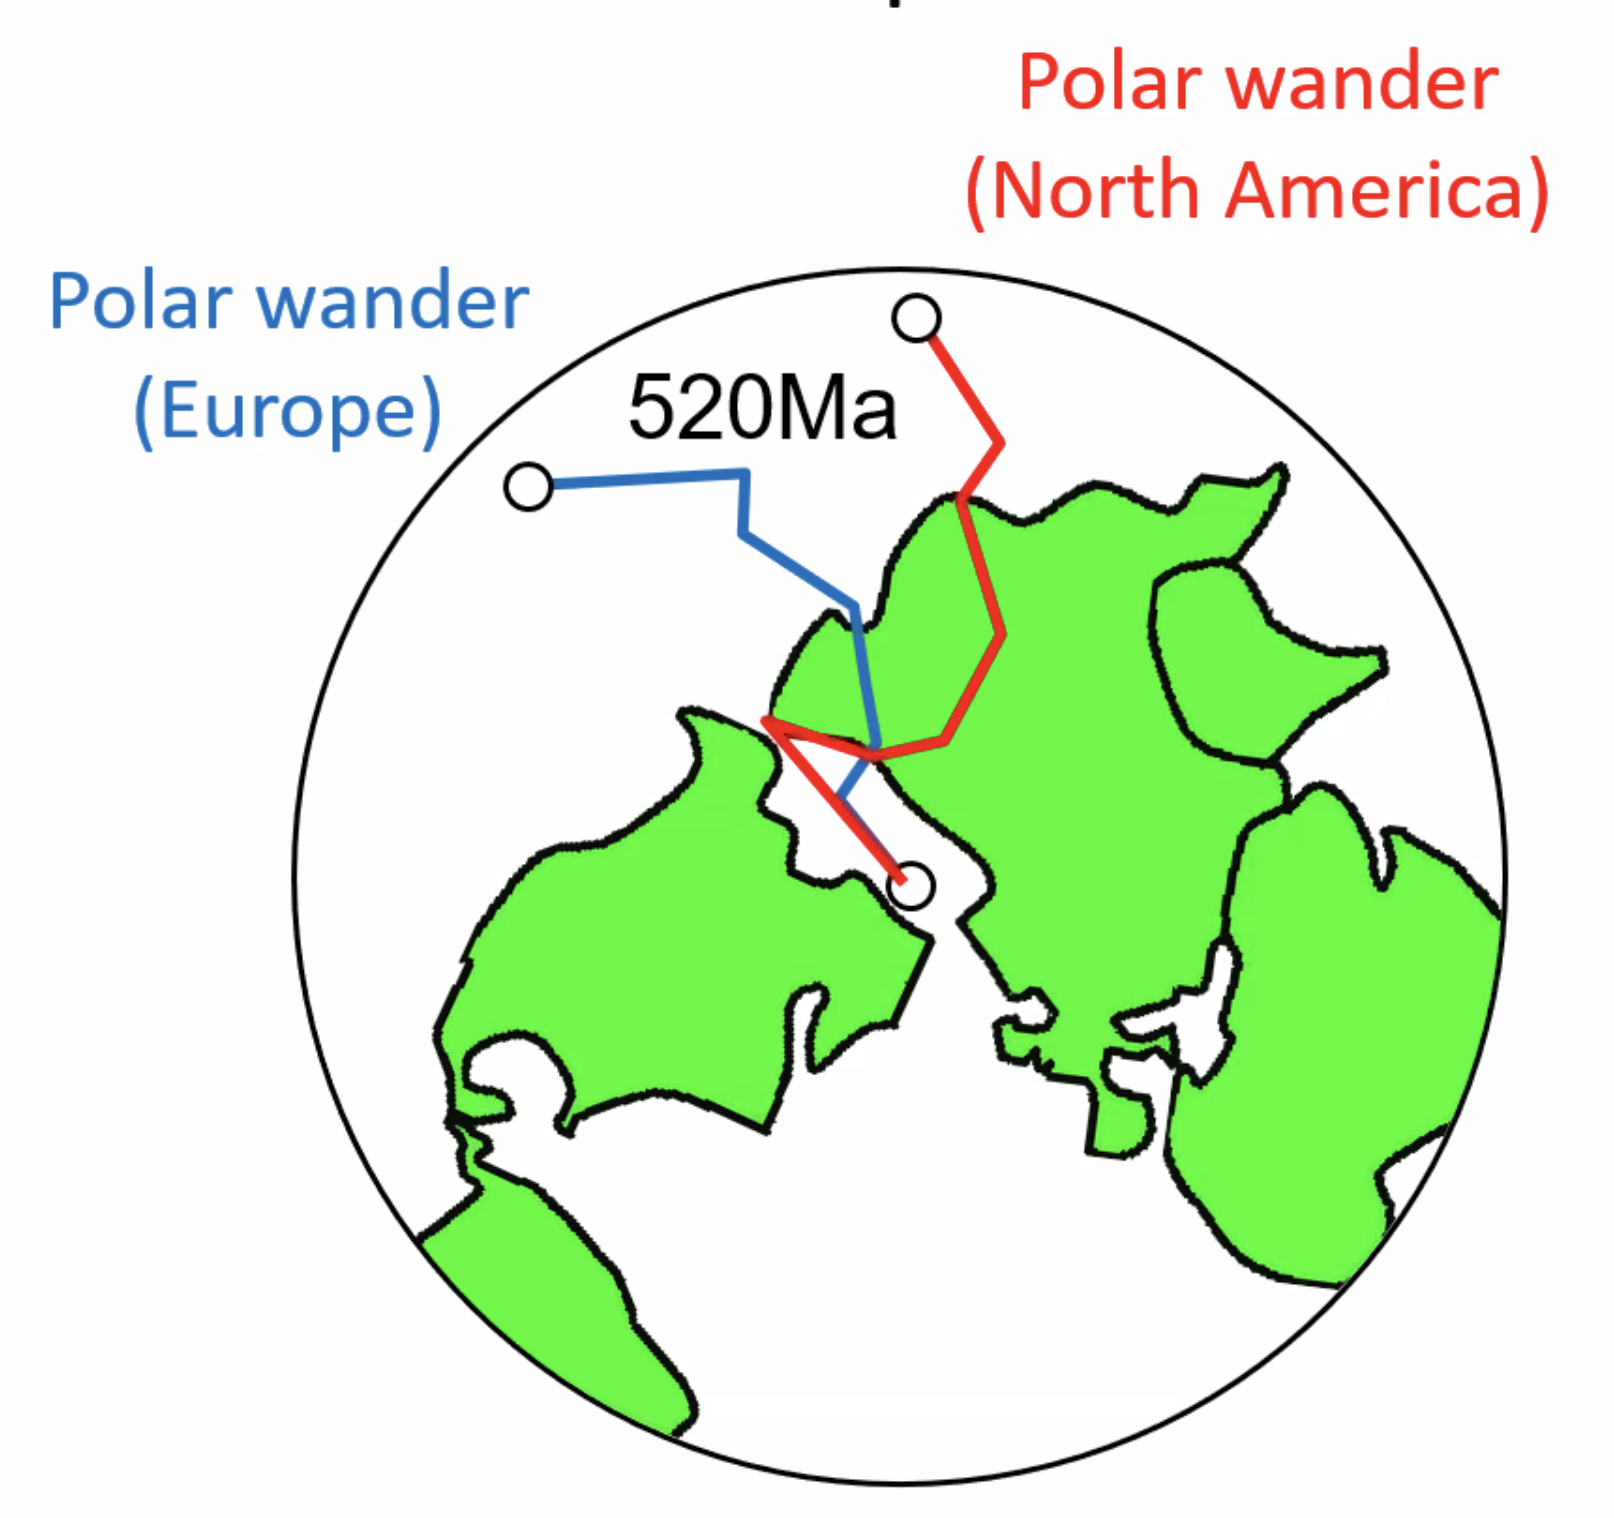
\includegraphics[width=0.5\linewidth]{content/img/polar_wander.png}
\end{figure}

\subsection{Ocean spreading}

Chicken and egg question: is the floor spreading because of volcanism, or is
the lava flowing because of spreading?

\begin{figure}[H]
    \centering
    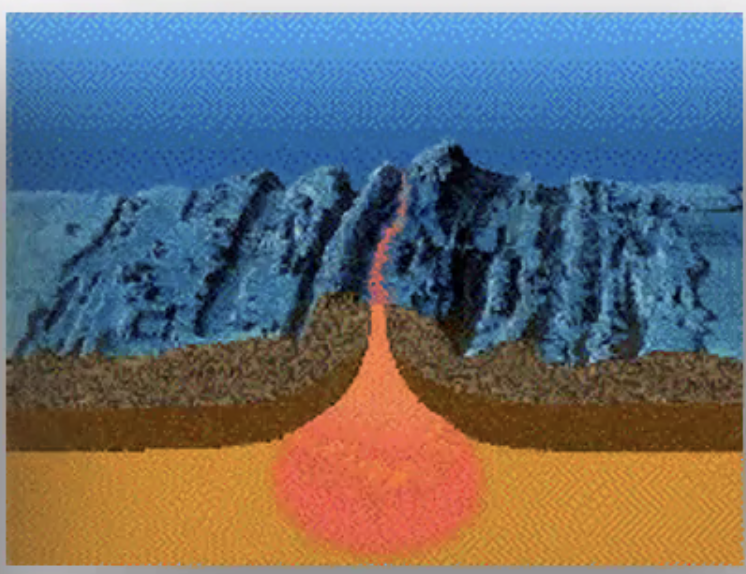
\includegraphics[width=0.5\linewidth]{content/img/ocean_floor_spreading.png}
\end{figure}

Ocean spreading increases CO$_2$ in the atmosphere (increased volcanism).
Mountain building does the opposite (more rocks for weathering).

\subsection{BLAG hypothesis}

\begin{figure}[H]
    \centering
    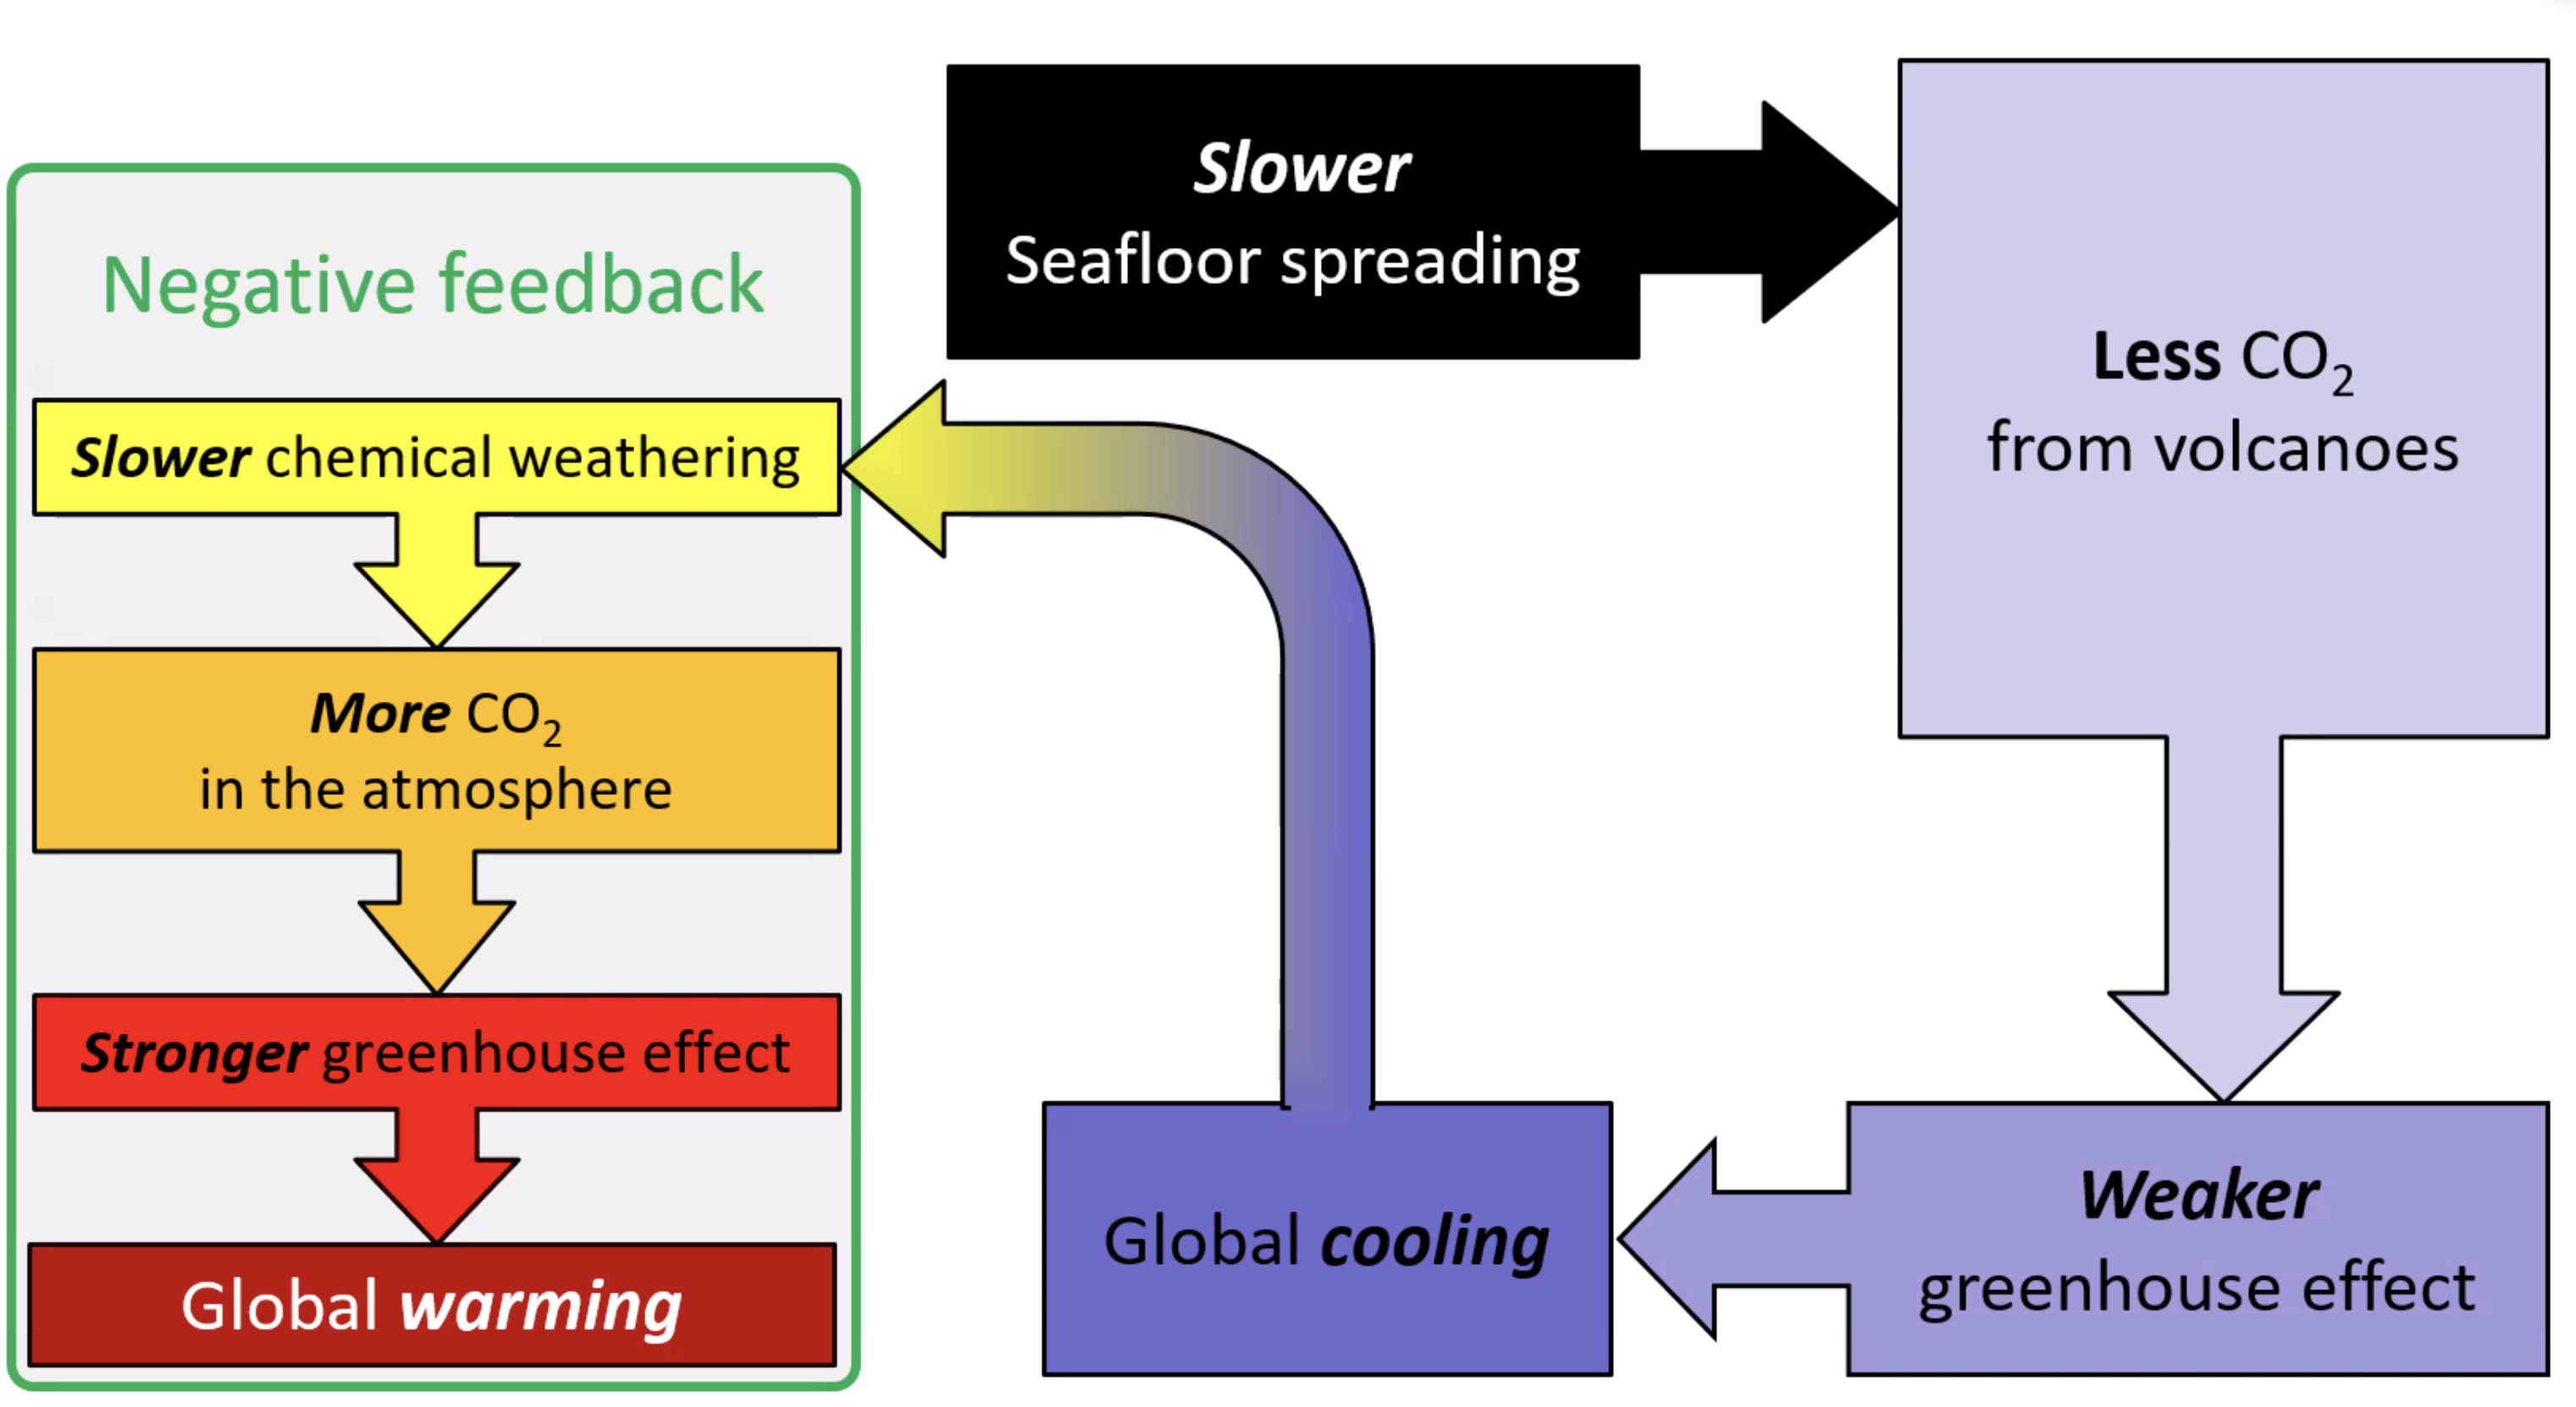
\includegraphics[width=\linewidth]{content/img/blag.png}
\end{figure}

\subsection{Uplift weathering hypothesis}

\begin{figure}[H]
    \centering
    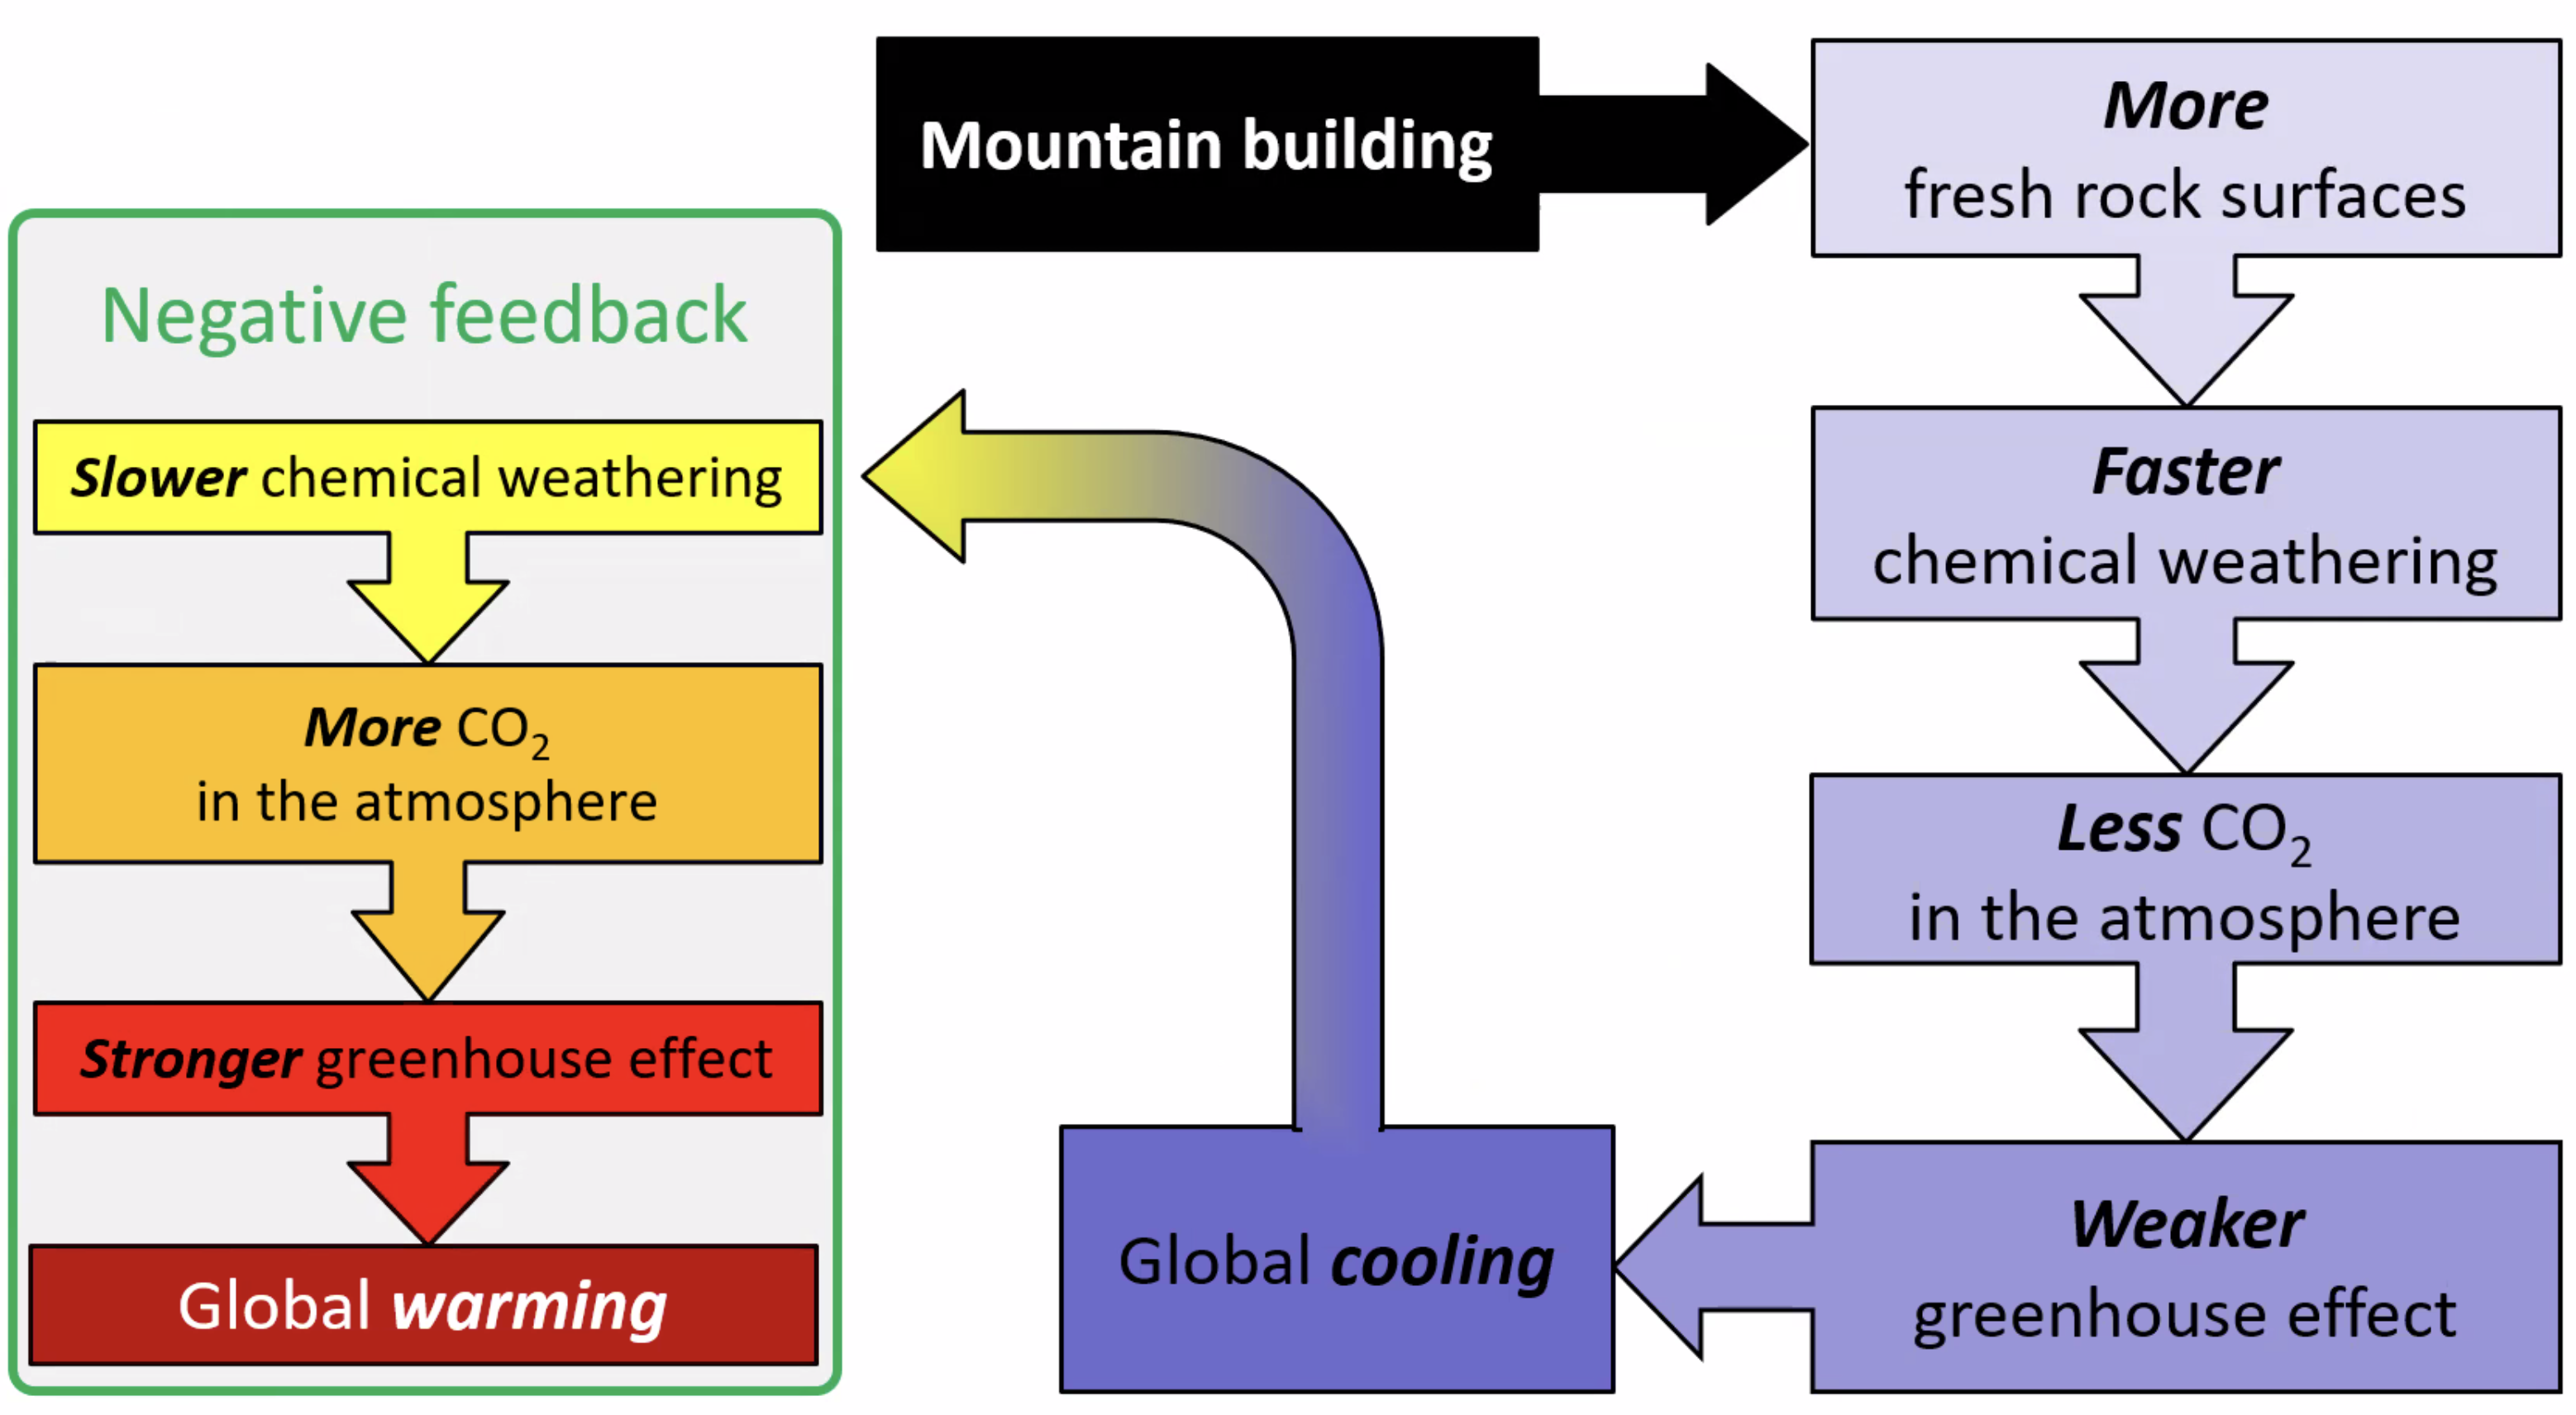
\includegraphics[width=1\linewidth]{content//img/uplift_weathering.png}
\end{figure}

\subsection{Polar position hypothesis}

Ice forms easier on land than on sea, which is the basis for polar position
hypothesis.

\begin{figure}[H]
    \centering
    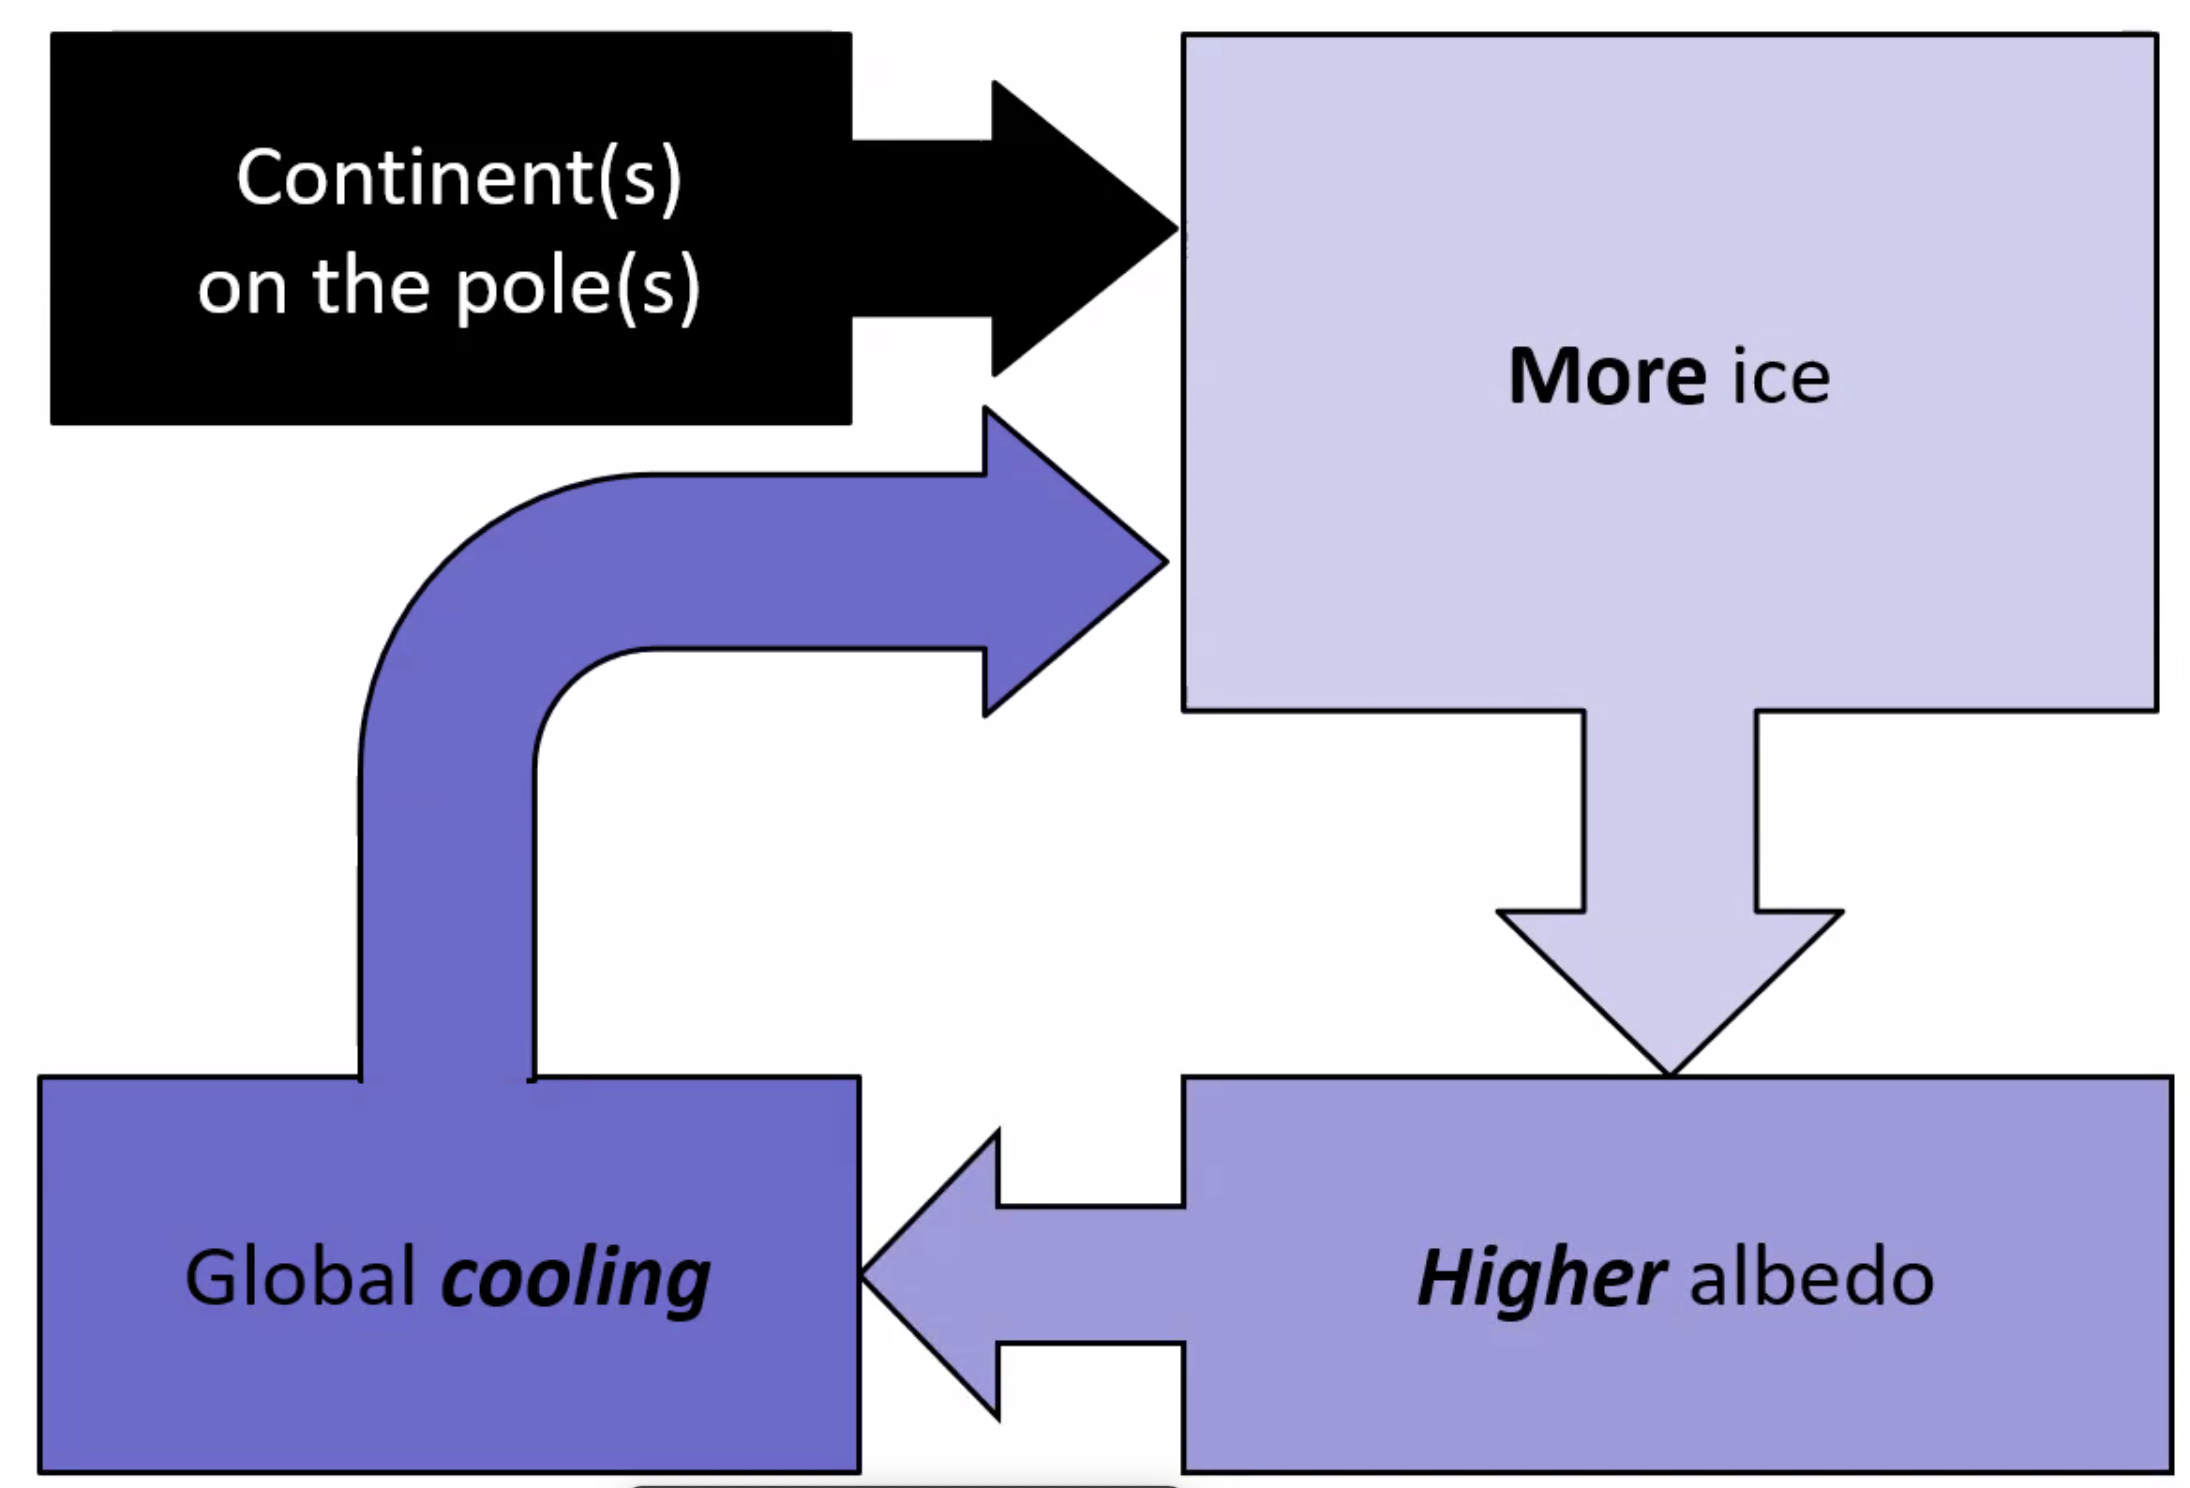
\includegraphics[width=1\linewidth]{
    content/img/polar_position_hypothesis.png}
\end{figure}

\subsection{Plate tectonics and climate}

\begin{itemize}
    \item \textbf{BLAG hypothesis}: slower seafloor spreading causes global
    cooling
    \item \textbf{Mountain building hypothesis}: mountain building causes
    global cooling
    \item \textbf{Polar position hypothesis}: land in polar positions causes
    global cooling
\end{itemize}

A continent (Antarctica) is on the South Pole, seafloor spreading is slow and
mountain building is ongoing forming the Himalaya. All these 3 suggest that the
climate should be cooling, not warming (when considering plate tectonics in
isolation).

%%%%%%%%%%%%%%%%%%%%%%%%%%%%%%%%%%%%%%%%%%%%%%%%%%%%%%%%%%%%%%%%%%%%%%%%%%%%%%%%
%%%%%%%%%%%%%%%%%%%%%%%%%%%%%%%%%%%%%%%%%%%%%%%%%%%%%%%%%%%%%%%%%%%%%%%%%%%%%%%%

\section{Reading assignment 5: Snowball Earth by Paul F. Hoffman and Daniel
P. Schrag}

Between 750 Myr ago and 580 Myr ago 4 drastic climate reversals happened,
between icehouse and hothouse.

\textbf{Neoproterozoic} are spans from 1 Byr to 538.8 Myr ago.

Occurrence of glacial debris near sea level in the tropics.

Earth's landmasses were most likely clustered near the equator during the global
glaciations that took place around 600 million years ago.

Albedo: ice sheets reflect more of Sun's energy than dark seawater.

Budyko's climate model:
\textit{
But his climate simulations also revealed that this feedback can run out of
control. When ice formed at latitudes lower than around 30 degrees north or
south of the equator, the planet’s albedo began to rise at a faster rate
because direct sunlight was striking a larger surface area of ice per degree
of latitude. The feedback became so strong in his simulation that surface
temperatures plummeted and the entire planet froze over.
}

However, according to his model, the albedo feedback should have gotten out of
control and extinguished all life on Earth.

\textit{
The first of these objections began to fade in the late 1970s with the
discovery of remarkable communities of organisms living in places once
thought too harsh to harbor life. Seafloor hot springs support microbes that
thrive on chemicals rather than sunlight. The kind of volcanic activity that
feeds the hot springs would have continued unabated in a snowball earth.
Survival prospects seem even rosier for psychrophilic, or cold-loving,
organisms of the kind living today in the intensely cold and dry mountain
valleys of East Antarctica. Cyanobacteria and certain kinds of algae occupy
habitats such as snow, porous rock and the surfaces of dust particles encased
in floating ice.
}

\textit{
In 1992 Joseph L. Kirschvink, a geobiologist at the California Institute of
Technology, pointed out that during a global glaciation, an event he termed a
snowball earth, shifting tectonic plates would continue to build volcanoes and
to supply the atmosphere with carbon dioxide. At the same time, the liquid
water needed to erode rocks and bury the carbon would be trapped in ice.
With nowhere to go, carbon dioxide would collect to incredibly high levels,
high enough, Kirschvink proposed, to heat the planet and end the global freeze.
}

\textbf{4 stages of Snowball Earth}
\begin{itemize}
    \item \textbf{Snowball Earth Prologue}
    \item \textbf{Snowball Earth at its coldest}
    \item \textbf{Snowball Earth as it thaws}
    \item \textbf{Hothouse aftermath}
\end{itemize}

%%%%%%%%%%%%%%%%%%%%%%%%%%%%%%%%%%%%%%%%%%%%%%%%%%%%%%%%%%%%%%%%%%%%%%%%%%%%%%%%
%%%%%%%%%%%%%%%%%%%%%%%%%%%%%%%%%%%%%%%%%%%%%%%%%%%%%%%%%%%%%%%%%%%%%%%%%%%%%%%%

\section{Lecture 5: Snowball Earth}

\textbf{We don't know if it actually happened.}

Scientists agree there was a major change in Earth's climate. Disputes concern
how major.

\subsection{Carbon isotope fractionation}

Bacteria take the lighter isotope $^{12}$C out of water and preferentially
leave out $^{13}$C.

"Default" value for $\delta^{13}$C is -6 (when no factors affect it).
Values of $\delta^{13}$C equal or below -6 mean there is no life at all.

When organic material intakes $^{12}$C, the $\delta^{13}$C in the surrounding
water increases.

\subsection{Port Askaig Tillite Formation, Islay}

\textit{...the material of which the mass is composed have in time, deeper than
we have hitherto suspected, been transported by the agency of ice.} - James
Thomson, F.G.S. 1871 on the stratified rocks of Islay

\subsection{Sturtian (718-658 Myr) and Marinoan (650-635 Myr)}

Similar glaciar rocks as found by Thomson were found everywhere, not only
on Islay. This is surprising because what would glaciar rocks do e.g. in
Australia?

\textbf{Howchin (1908): Sturtian Formation in Sturt river,
Austrailia}

\textbf{isräfflor} - scratches on rocks done by glaciers.

\textbf{Mawson (1949): Elatina Formation, Australia}

\textit{Records of severe glaciation in the late Precambrian are fast
accumulating. So far as can at present be judged, frequent and widespread
refrigerations were a feature of at least middle to late Proterozoic time.
Glaciation is evidenced to the Equators itself.
}
%%%%%%%%%%%%%%%%%%%%%%%%%%%%%%%%%%%%%%%%%%%%%%%%%%%%%%%%%%%%%%%%%%%%%%%%%%%%%%%%
\subsection{Paleomagnetic studies of Gondwana during the Neoproterozoic Era}
Neoproterozoic\footnote{1 billion to 538.8 million years ago}

\begin{figure}[H]
    \centering
    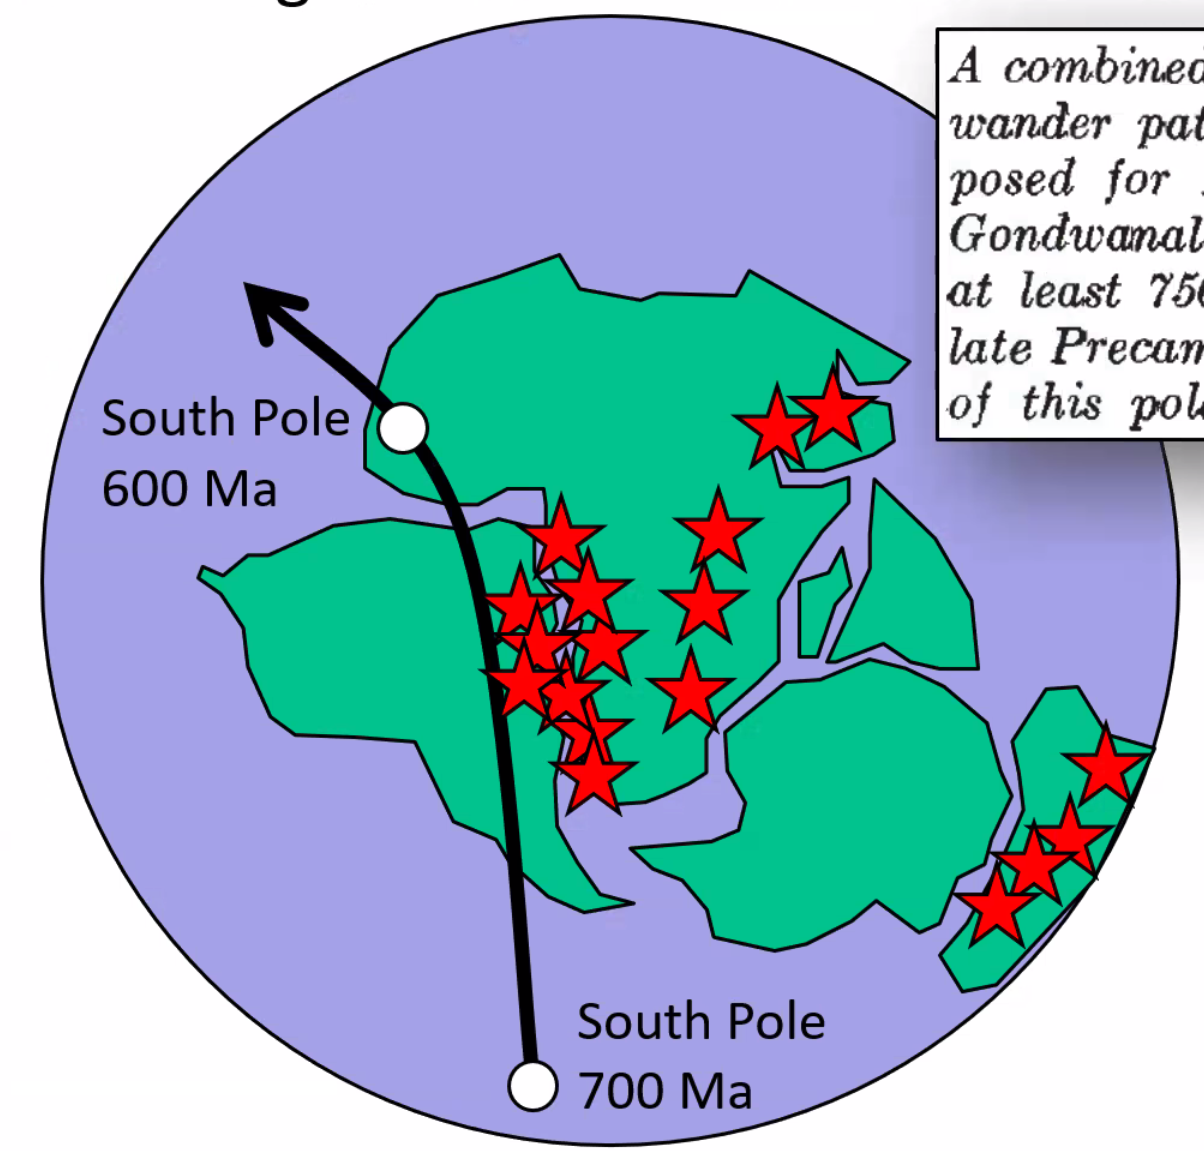
\includegraphics[width=0.75\linewidth]{content/img/gondwana.png}
\end{figure}

\begin{figure}[H]
    \centering
    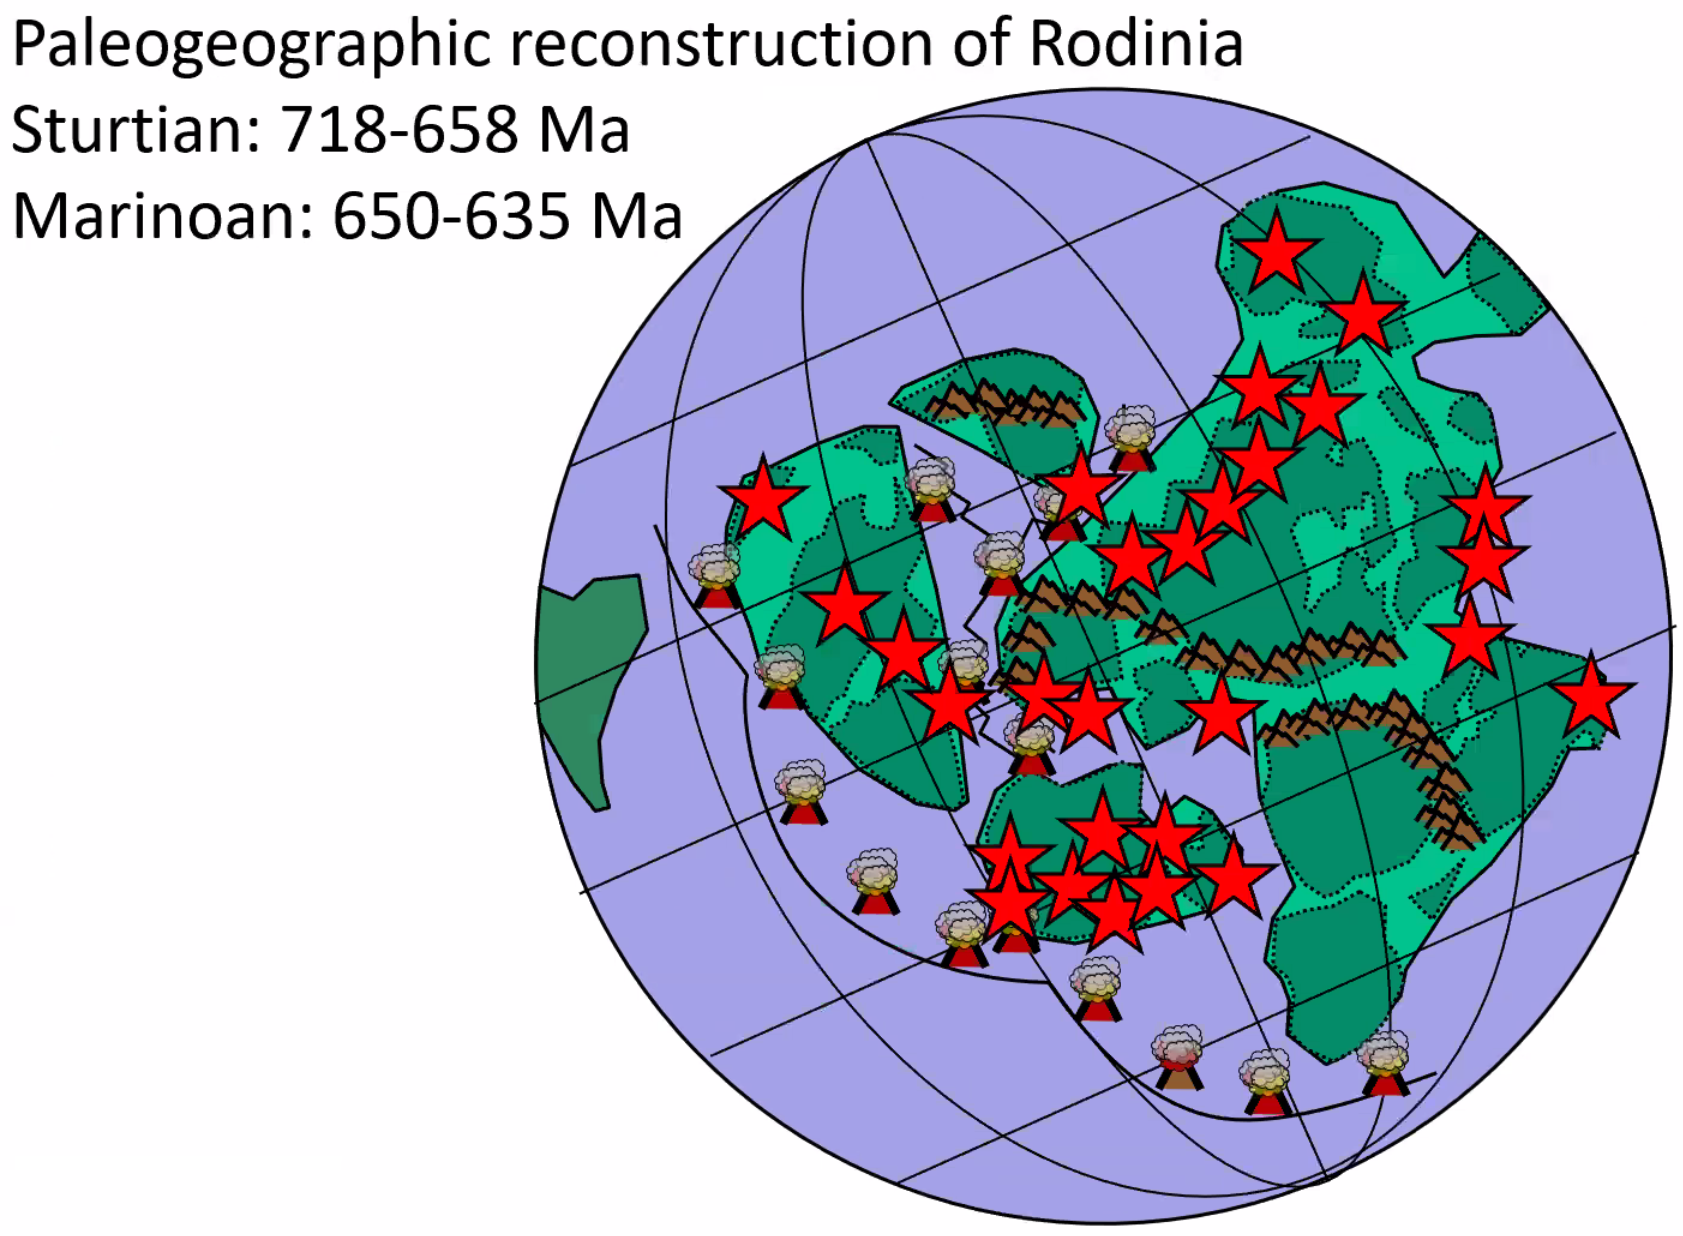
\includegraphics[width=0.75\linewidth]{
    content/img/rodinia_snowball_earth.png}
\end{figure}

So how do we get the glaciers at the equator?

How about \textbf{axial tilt?} It would need to be bigger than $54 \degree$
for the equator to be cooler than the poles. And it wouldn't explain why it
happened twice.

\subsection{Ghaub Formation, Namibia}

\textbf{Till}\footnote{
Till or glacial till is unsorted glacial sediment.

Till is derived from the erosion and entrainment of material by the moving
ice of a glacier. It is deposited some distance down-ice to form terminal,
lateral, medial and ground moraines.

Till is classified into primary deposits, laid down directly by glaciers,
and secondary deposits, reworked by fluvial transport and other processes.
}

\textbf{Cap carbonate}\footnote{
Cap carbonates are layers of distinctively textured carbonate rocks
(either limestone or dolomite) that occur at the uppermost layer of
sedimentary sequences reflecting major glaciations in the geological record.
}

%%%%%%%%%%%%%%%%%%%%%%%%%%%%%%%%%%%%%%%%%%%%%%%%%%%%%%%%%%%%%%%%%%%%%%%%%%%%%%%%
\begin{figure}[H]
    \centering
    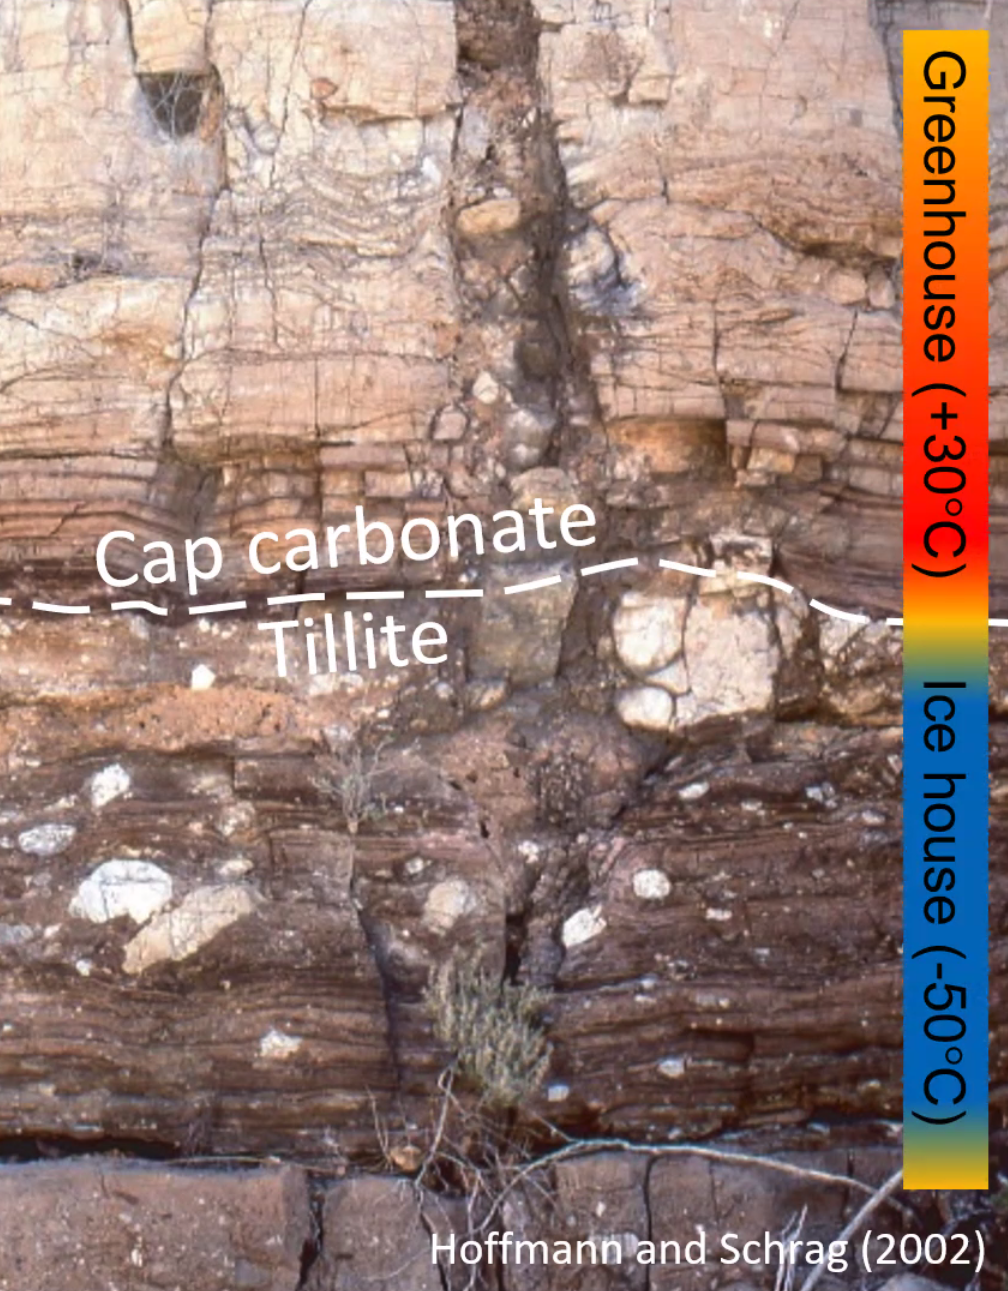
\includegraphics[width=0.75\linewidth]{
    content/img/tillite_and_cap_carbonate.png}
\end{figure}

\subsection{Snowball Earth hypothesis}

Kirschvink (1992) first made the hypothesis but Hoffman popularized it.

Continents in the tropics (with no vegetation because it hadn't evolved yet)
$\rightarrow$
Higher albedo (desert with no vegetation has higher albedo than ocean water)

Mountain building in the tropics $\rightarrow$ Faster weathering

Higher albedo + Faster weathering $\rightarrow$ Earth becomes \textbf{much}
cooler $\rightarrow$ glaciation in the tropics $\rightarrow$ \textbf{even}
higher albedo $\rightarrow$ \textbf{even} faster cooling
$\rightarrow$ Snowball Earth

CO$_2$ from volcanoes $\rightarrow$ increased GH effect

Ash particles from volcanoes $\rightarrow$ Lower albedo

Lower albedo + increased GH effect $\rightarrow$ Earth becomes \textbf{much}
warmer $\rightarrow$ Ice melts $\rightarrow$ \textbf{Even} lower albedo
$\rightarrow$ Ice melts \textbf{faster} $\rightarrow$ Extreme GH

%%%%%%%%%%%%%%%%%%%%%%%%%%%%%%%%%%%%%%%%%%%%%%%%%%%%%%%%%%%%%%%%%%%%%%%%%%%%%%%%

\subsection{Solar radiation}

$T = (E/\delta)^{1/4}$

$E = 342 W.m^{-2}$

$\delta = 5.670367 \times 10^{-8} W.m^{-2}.K^{-4}$

$T = 6\degree$C

Earth's albedo is $\alpha = 30$\% which equals $103W.m^{-2}$

Then the energy left gives $-18\degree$C. GHG contribute $+32\degree$C

\subsection{Solar radiation (716 Myr ago = Onset of Snowball Earth)}

Albedo between 50-95\%. Volcanic ash on ice sheets decreases the albedo.

$E = 160 W.m^{-2}$

$T = -43 \degree$

\subsection{Greenhouse effect (658 Myr = End of Snowball Earth)}

We're looking for how much CO$_2$ would be needed in the atmosphere to exit
the Snowball Earth. Currently (pre-industrial) at 280 ppm the GHG contribute
$32 \degree$ to global temperature.

$\Delta T = 4.3 \ln (C/C_0)$

For 1000 ppm: $\Delta T = 4.3 \ln (1000/280) = 5.5 \degree$

For 10000 ppm: $\Delta T = 4.3 \ln (10000/280) = 15.4 \degree$

For 100000 ppm: $\Delta T = 4.3 \ln (100000/280) = 25.27 \degree$

$T = -11 \degree + 25.c \degree = 14.3 \degree$ at 100000 ppm (10\%
CO$_2$ in the atmosphere)

\subsection{Cap carbonate}

Ca + Mg + CO$_2$ $\rightarrow$ CaMg(CO$_3$)$_2$

\subsection{Iron formations}

Fe + O$_2$ $\rightarrow$ Fe$_2$O$_3$

\section{Reading assignment: The Paleocene-Eocene Thermal Maximum: A
Perturbation of Carbon Cycle, Climate, and Biosphere with Implications for the
Future}

\textbf{PETM}: Paleocene-Eocene Thermal Maximum, ca. 56 Myr ago

Period of carbon release below 20k years, the whole event lasted about 200k
years. The global temperature increase was $5-8 \degree$.

Kenneth and Stott 1991:
\begin{itemize}
	\item Ocean Drilling Program 690 off the coast of Antarctica
	\item Decline in oxygen isotope ratios indicating warming
	$3-4 \degree$ in surface water and $6 \degree$ in deep water
	\item Negative shift in $\delta^{13}C$ of benthic and planktic forams
	\item Rapid onset of the event, around 6k yrs
\end{itemize}

\textbf{CIE}: Carbon Isotopic Excursion

Dating CIE onset:

\begin{itemize}
	\item Using radiometric dates of marine ash layers and orbital tunings
	of marine sediments
	\item Dated around 56.011-56.293 Ma.
	\item Orbital timescales suggest total duration of 150-220 ka.
\end{itemize}

The PETM is defined by a global temperature rise that was initially inferred
from a $> 1$‰ negative excursion in in $\delta^{18}O$ of benthic foraminifera,
indicating a deep-water temperature increase of $5\degree$C.

A similar warming was inferred from the Mg/Ca ratios.

The absence of warming during PETM at polar latitudes implies lack of
ice-albedo feedback loop.

Indicators of massive carbon release at PETM:

\begin{itemize}
	\item large global negative CIE
	\item extensive dissolution of deep-ocean carbonates
\end{itemize}

\textit{The negative shift in carbon
isotope ($\delta^{13}$C) values shows that the carbon released was depleted in
$^{13}$C relative to the exogenic reservoir (ocean + atmosphere + biomass) and
was likely organic carbon because organisms discriminate against
$^{13}$C during biosynthesis.} The rapid onset (<20ka) indicates addition of
$^{13}$C-depleted carbon rather than reduction in organic carbon burial (100ka
timescale).

\subsection{Summary points}

1.The Paleocene-Eocene Thermal Maximum, which took place around 56 Mya and
lasted for around 200 ka, stands as the most dramatic geological confirmation
of the greenhouse theory -- increased CO$_2$ in the atmosphere warmed Earth's
surface.

2. The large release of organic $^{13}$C-depleted carbon caused a global
carbon isotopic excursion, widespread deep-ocean acidification, and carbonate
dissolution.

3. Carbon was removed from the exogenic pool on a timescale of 100 ka,
primarily through silicate weathering and eventual precipitation of carbonate
in the ocean and/or uptake by the biosphere and subsequent burial as organic
carbon.

4. Warming associated with the carbon release implies approximately two
doublings of atmospheric $p$CO$_2$ unless climate sensitivity was significantly
different during the Paleogene.

5. Although there was a major extinction of benthic foraminifera, most groups
of organisms did not suffer a mass extinction.

6. Geographic distributions of most kinds of organisms were radically
rearranged by $5-8 \degree$C of warming, with tropical forms moving poleward
in both maritime and terrestial realms.

7. Rapid morphological change occured in both maritime and terrestrial lineages
suggesting that organisms adjusted to climate change through evolution as well
as dispersal and local extirpation. Where best understood, these evolutionary
changes appear to be a response to nutrient and /or food limitation.

8. Research of the PETM and other intervals of rapid global change has been
driven by the idea that they provide geological parallels to future
anthropogenic warming, but much remains to be done to gain information that can
be acted on.


%%%%%%%%%%%%%%%%%%%%%%%%%%%%%%%%%%%%%%%%%%%%%%%%%%%%%%%%%%%%%%%%%%%%%%%%%%%%%%%%
\section{Lecture 6: Paleocene-Eocene Thermal Maximum}

Snowball Earth won't happen again because of vegetation it would be
very hard to get that albedo effect.

The brown section in sediment blocks from Ocean Drilling Program is pure clay,
corresponding to a period without deep marine life.

\textbf{Cenozoic Era} is the last 66 Myr, from the last major extinction to
the present day.

\begin{figure}[H]
    \centering
    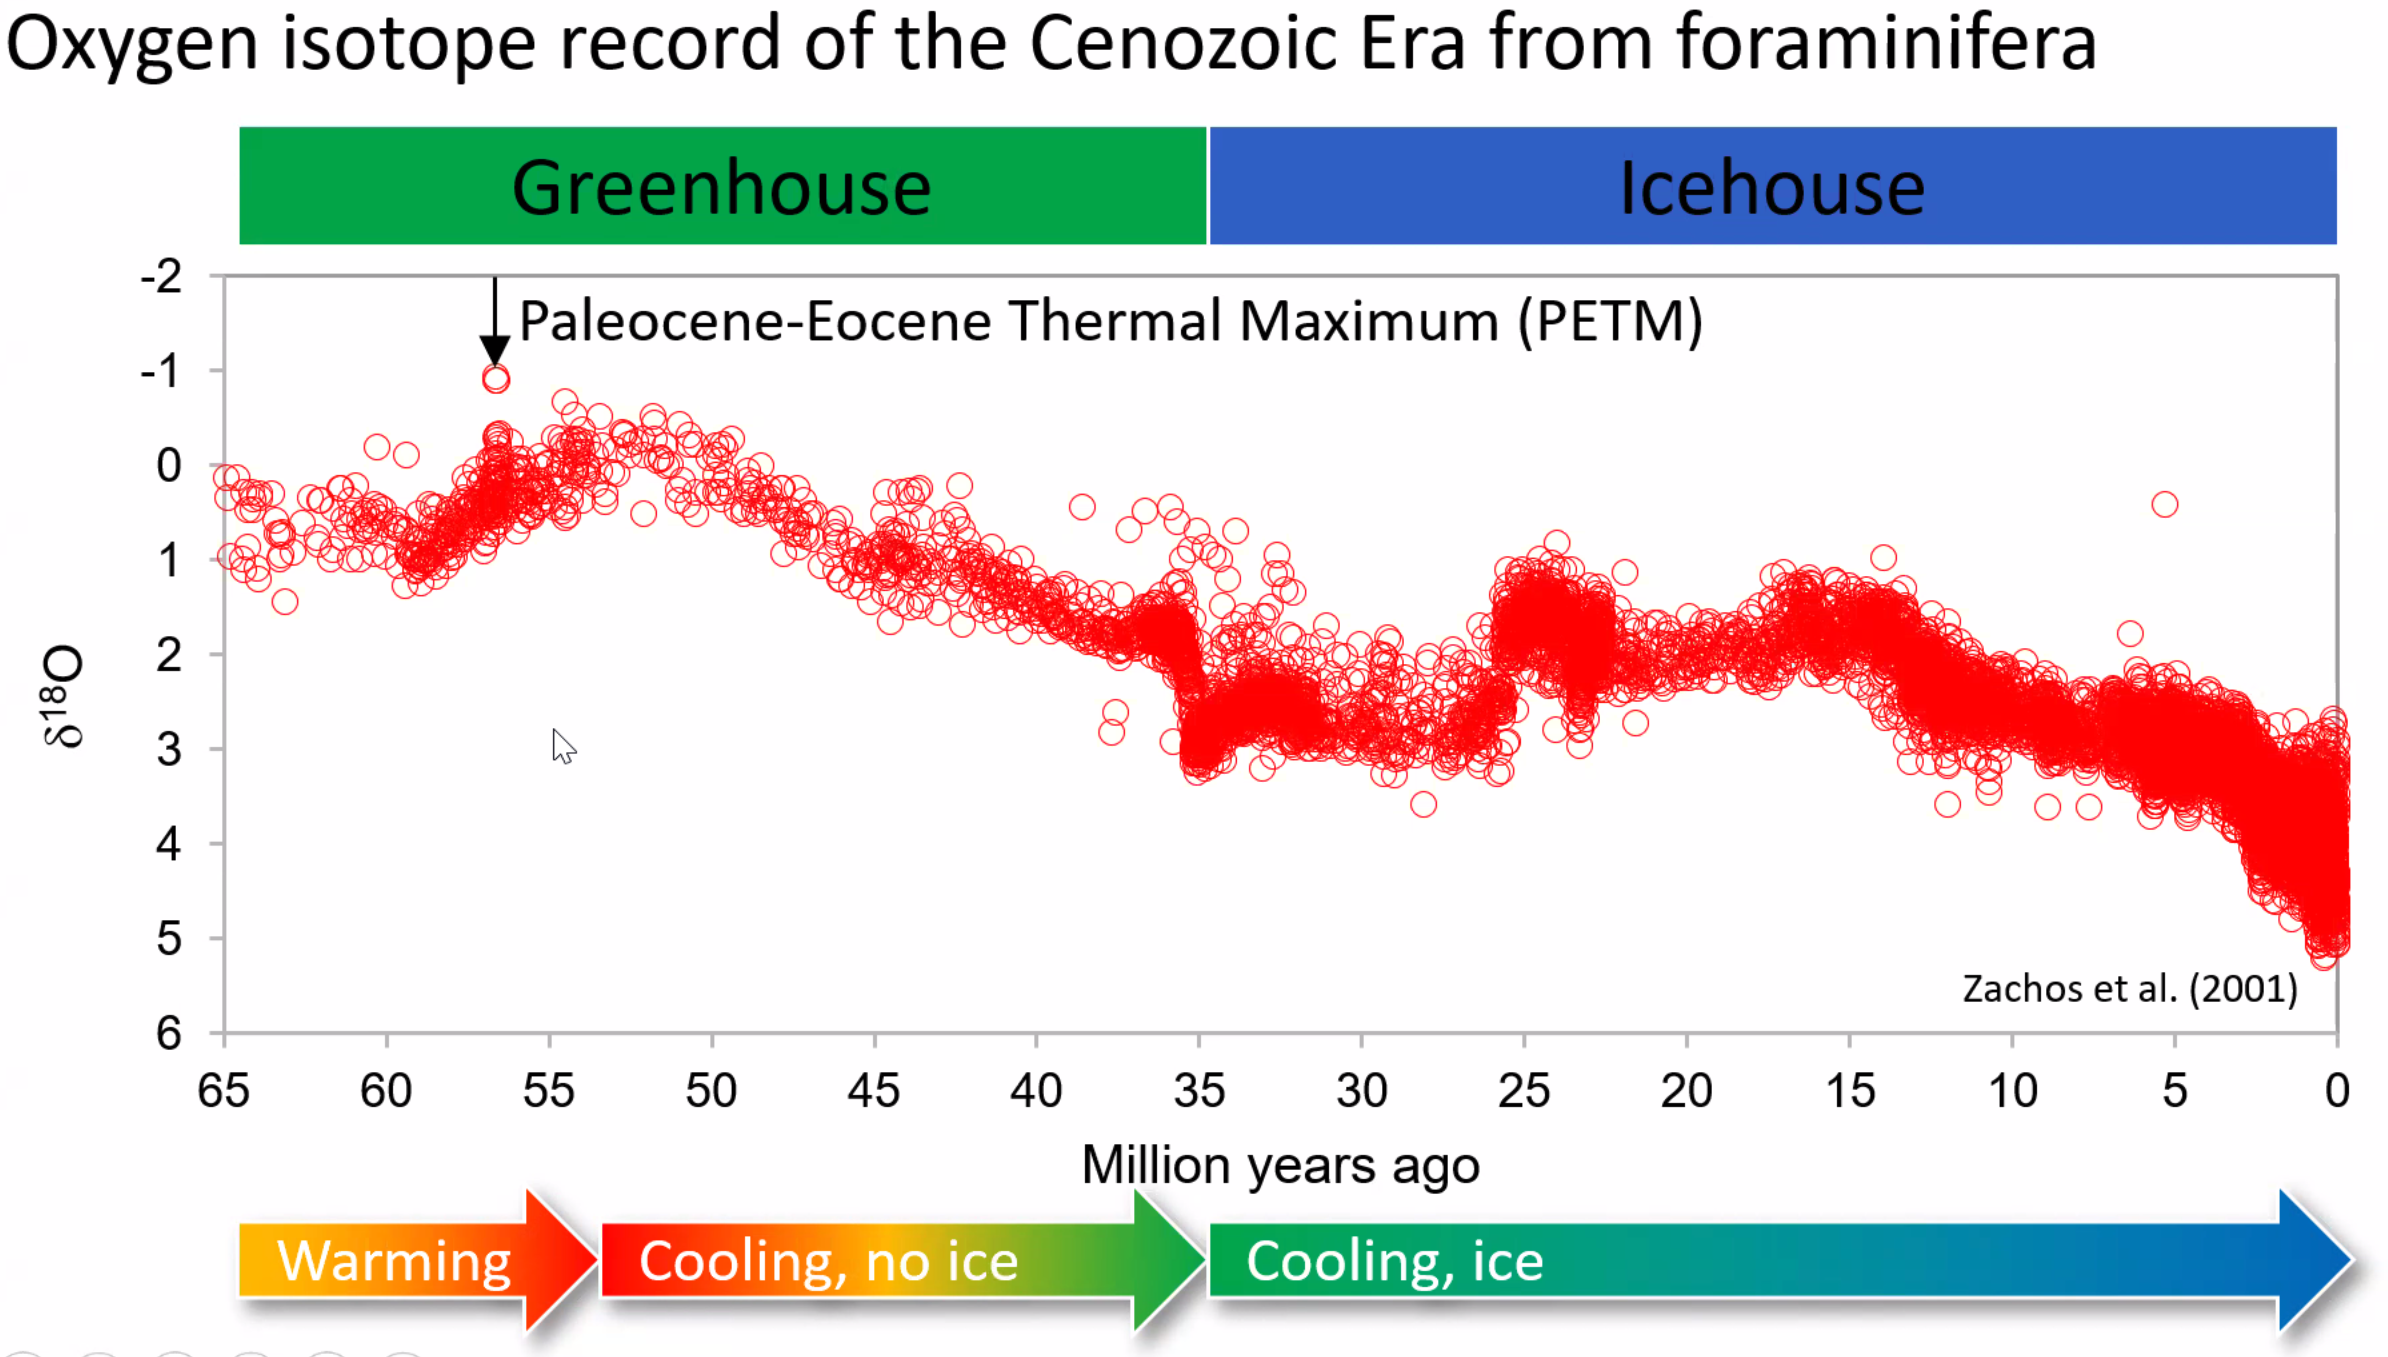
\includegraphics[width=0.95\linewidth]
    {content/img/cenozoic_isotope_record_from_forams.png}
\end{figure}

If we zoom into the above graph, the spike is very sudden, on a scale of 1 Myr.
$\delta^{18}$O changes from 0.5 to -1.

$\Delta T = 4.2[\delta^{18}O_1 - \delta^{18}O_2]$

$\Delta T = 4.2[1.5] = 6.3 \degree$

So what we observe is a temperature change of $+6.3 \degree$. We're currently
experiencing a world $1.5 \degree$ warmer than it should be.

We see the effect of \textbf{extreme warming} in the marine life -- there seems
to be absence of forams sediments in that period of time. The warming is clearly
correlated with a mass extinction.

\subsection{Cerrejon mine, Colombia}

In this coal mine, researchers have found fossils of a snake \textit{titanoboa
cerrejonensis vertebrae}. The snake was \textit{massive}, much bigger than
Boa constrictor (3.4m).

\subsection{Titanoboa cerrejonensis as a paleothermometer}

Modern light green anaconda: 7.3m, living in mean annual temperature of
$27 \degree$C.

Titanaboa was at least 13m, living in $32-33 \degree$C.

(both measured at $5.5\degree$N).

Mean annual temperature at PETM was $39-40 \degree$C.

\subsection{Mean annual temperature and latitude}

In a warmer climate, temperature flattens out. We see it today, we call it
Arctic amplification. In the Arctic regions, warming is happening much faster
then elsewhere. In Svalbard, there's up to 10 degrees of warming.

\begin{figure}[H]
    \centering
    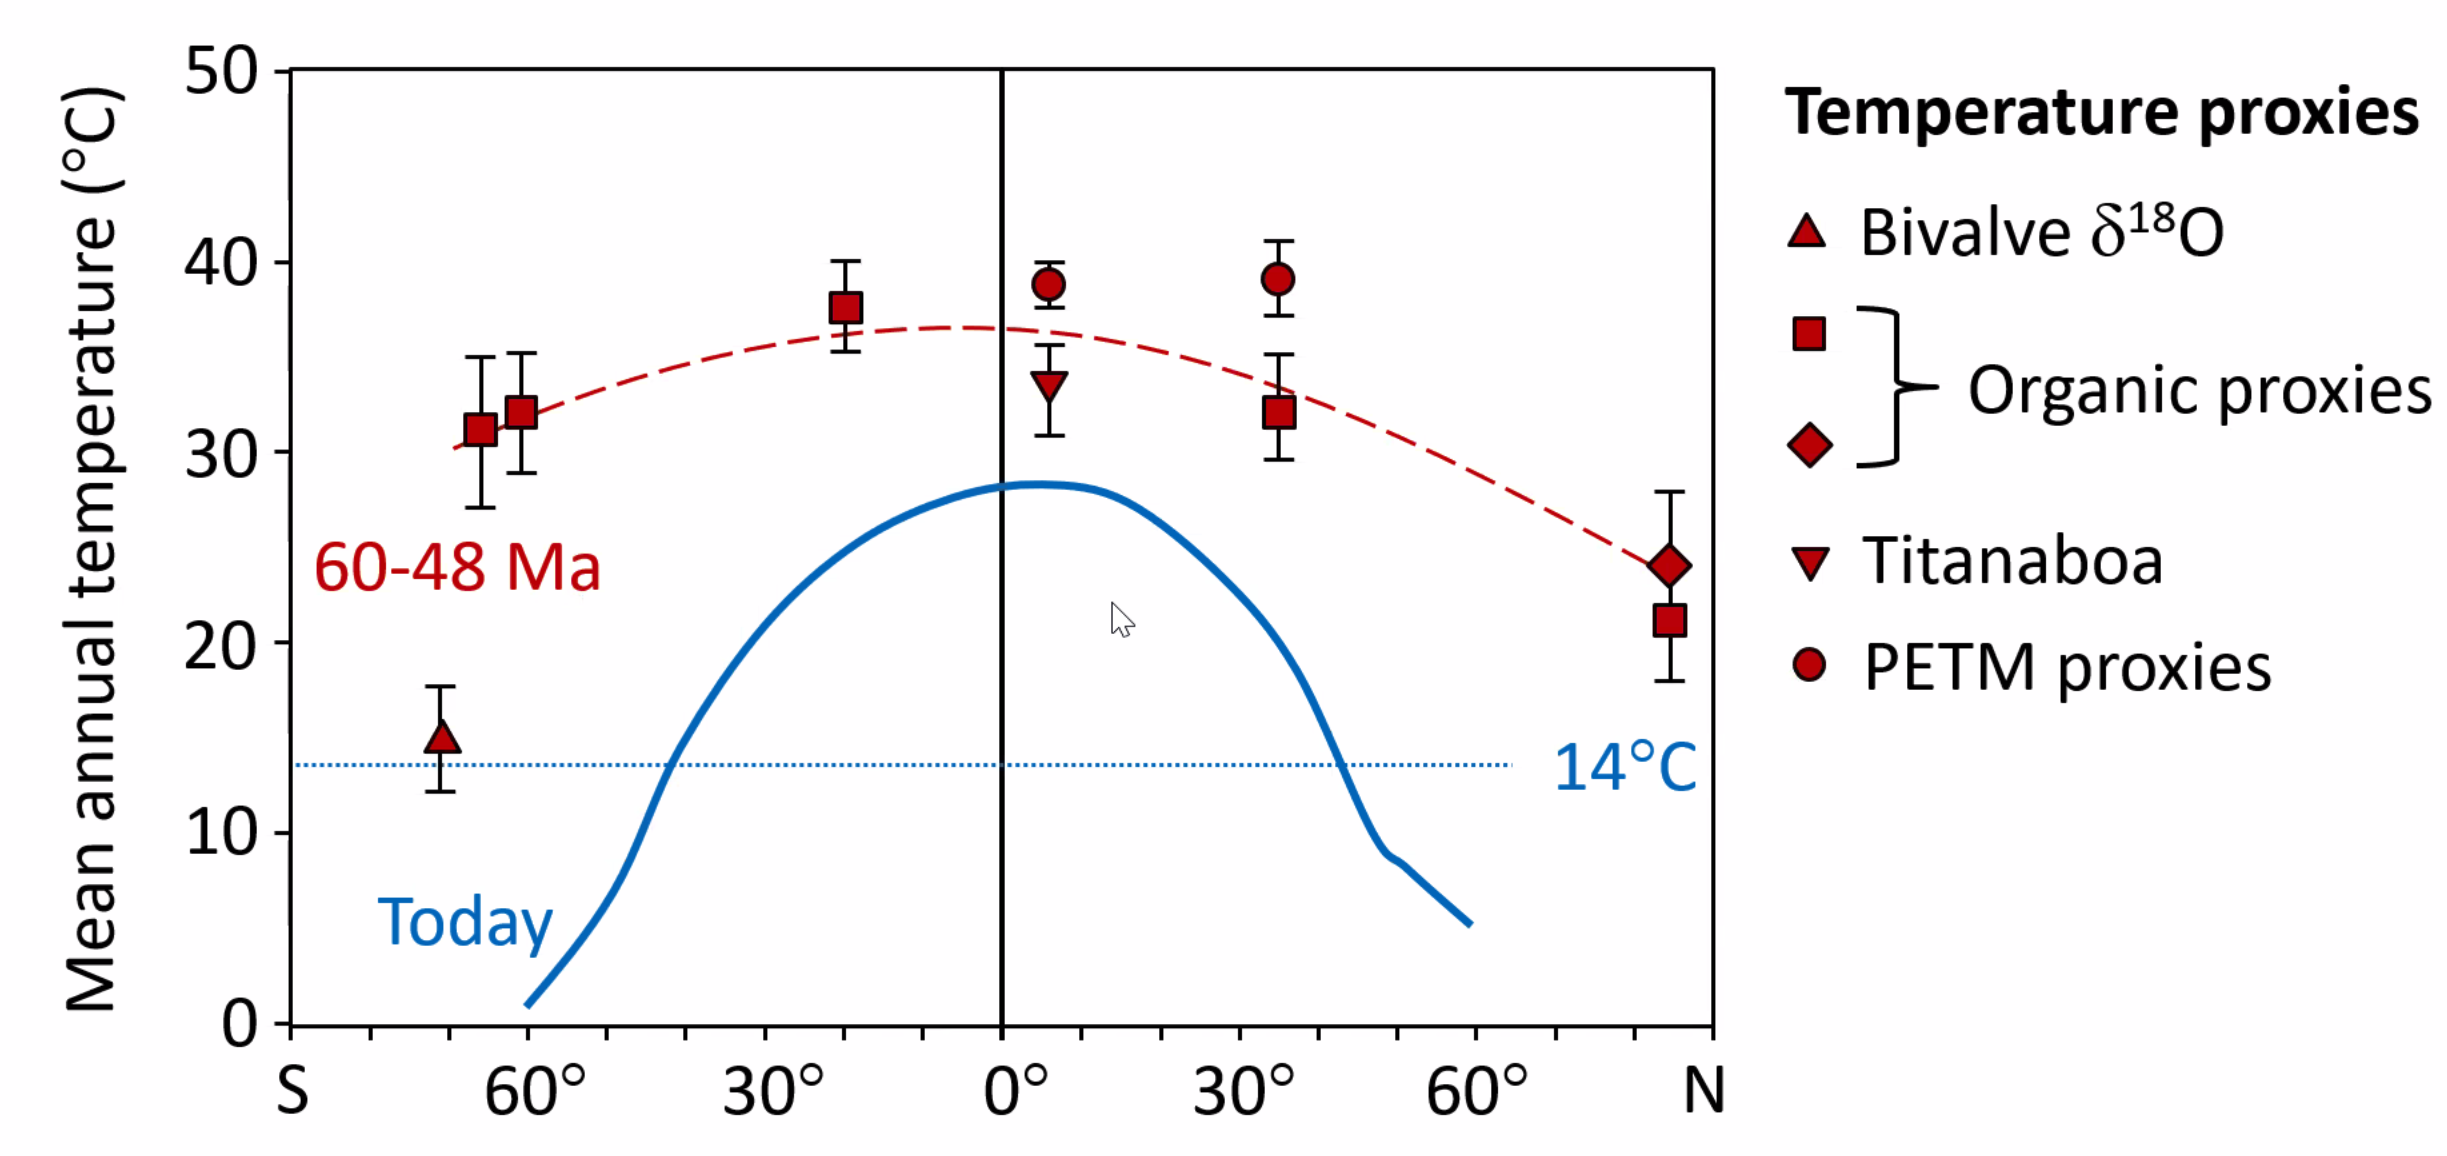
\includegraphics[width=0.75\linewidth]
    {content/img/temperature_proxies_warming.png}
\end{figure}

\subsection{Carbon isotope record: PETM}

Carbon isotope value becomes radically more negative at the PETM, mirroring the
oxygen data. Whatever was added to the ocean, must have a very negative
$\delta{13}C$.

Candidates:
\begin{itemize}
    \item Volcanoes ($CO_2$; $\delta{13}C = -6‰$)
    \item Methane from thawing of permafrost ($CH_4$; $\delta{13}C = -22‰$)
    \item Methane clathrates -- in sediments on
    a seafloor ($CH_4$; $\delta{13}C = -60‰$)
\end{itemize}

Was it a lot of volcanism, was it a fair amount of thawing permafrost, or was
it a little bit of methane clathrates?

$\delta^{13}C_{\text{source}} = [
(\delta^{13}C_2-\delta^{13}C_1) \times
(C_{\text{mass in ocean}} + C_{\text{mass added to ocean}})
-
(C_{\text{mass in ocean}} \times 1.5)
] / C_{\text{mass added to ocean}}$

We know the mass of carbon in the ocean to be 38700 billion tons.
We also know that $\delta^{13}C$ dropped from 1.5 to -1.5.

$\delta^{13}C_{\text{source}} = [
(-1.5-1.5) \times
(38700 + C_{\text{mass added to ocean}})
-
(38700 \times 1.5)
] / C_{\text{mass added to ocean}}$

Here's how much carbon we would need to add from different sources:

\begin{figure}[H]
    \centering
    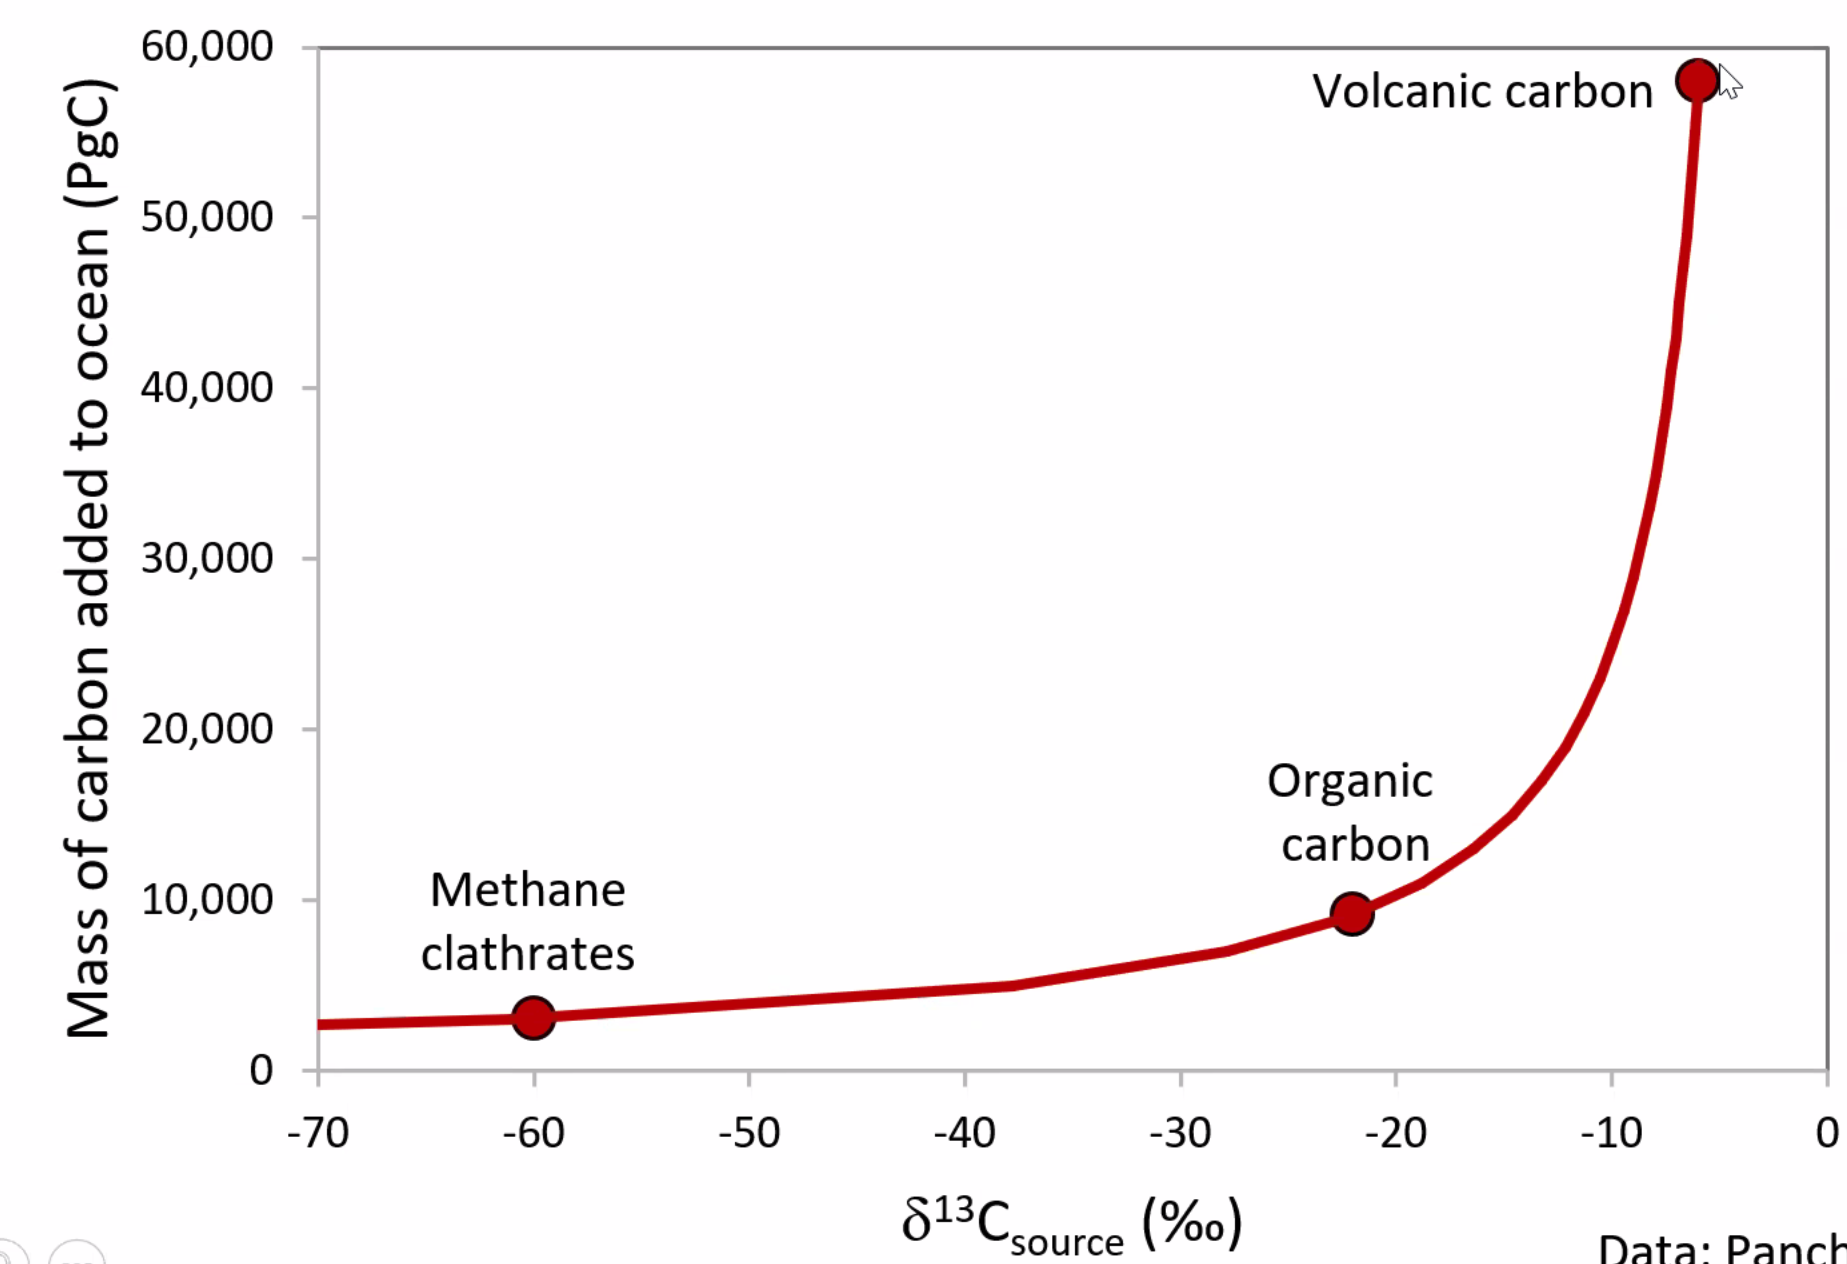
\includegraphics[width=0.75\linewidth]
    {content/img/adding_carbon_to_ocean.png}
\end{figure}

Researchers estimated that between 3000 PgC and 7126 PgC could have accumulated
in the ocean. This suggests that the likely source of carbon is not volcanoes,
simply not enough carbon is added. It must be one of the other two factors, or
the combination (thawing of permafrost or methane clathrates).

\subsection{Hypothesis}

More CO2 in the atmosphere and oceans because of volcanism
$\rightarrow$
Global warming
$\rightarrow$
Permafrost and/or methane clathrates thaw
$\rightarrow$
More CH$_4$/CO$_2$ in the atmosphere and oceans
$\rightarrow$
Greenhouse effect strengthens
$\rightarrow$
Global warming

The hypothesis is then that the \textbf{volcanism was the trigger} but the
thawing of permafrost and/or clathrates was the \textbf{feedback loop}.

\subsection{Carbonate Compensation Depth (CCD)}

CCD describes the depth at which the reaction swaps directions
$Ca^{2+} + 2 HCO_3^{-} \rightarrow CaCO_3 + CO2 + H_2O$\\
------------------------------ (CCD) --------------------------\\
$CaCO_3 + CO2 + H_2O \rightarrow Ca^{2+} + 2 HCO_3^{-}$

Beyond compensation depth, limestone dissolves.

When we add CO$_2$, the CCD rises to a higher level, because the bottom
reaction is favoured.

Currently, CCD is around 3500-4000 meters.

\subsection{Duration of PETM}

170000 years

That's how long it takes to recover after a perturbation of the carbon cycle.
That's important to know because people are perturbing the carbon cycle today.

\subsection{Bighorn Basin, Wyoming}
\begin{itemize}
    \item 5 species found only before PETM
    \item 22 species found before and after PETM
    \item 46 immigrant species during PETM
    \item 5 immigrant species after PETM
\end{itemize}

We're seeing this today, at $1.5 \degree$ warming, 2\% of species are heading
towards extinction.

%%%%%%%%%%%%%%%%%%%%%%%%%%%%%%%%%%%%%%%%%%%%%%%%%%%%%%%%%%%%%%%%%%%%%%%%%%%%%%%%
\section{Reading assignment: Chapter 19: Causes of Warming over the last 125
years}

\subsection{Natural causes of recent warming}
Changes over tectonic time scales are clearly irrelevant to the changes of the
last 125 years. Average rate of cooling during transitions between greenhouse
and icehouse conditions is $0.00001\degree$ per century).

Orbital forcing works at the rate of $0.00016 \degree$ per century or less.

\subsubsection{Solar forcing}

The amount of radiation arriving from the Sun varies in 11-year cycles changing
by a little over 1 W/m$^2$, equivalent to about $0.1\%$ of the global average.

\subsection{CO$_2$}

Bubbles of ancient air trapped in ice and direct measurements of air by the
geochemist Charles Keeling begun in 1958 show an accelerating rise in the
CO$_2$ concentration during the last two centuries. By 2010 the CO$_2$
concentrations had risen to 390 ppm, well above the 180-300ppm range of natural
(glacial-interglacial) variations.

On an annual average, cold high-latitude ocean water is a CO$_2$ sink and warm
low-latitude ocean is a CO$_2$ source.
One of the reasons is that CO$_2$ gas is more easily dissolved in cold water
than in warm water.

Greenhouse experiments show that most plants obtain carbon more effectively
from CO$_2$-rich atmosphere and grow faster as a result.

Ice core and instrumental measurements show that atmospheric CO$_2$ levels have
risen by almost $40\%$ in the last 150 years.

\subsection{Methane (CH$_4$)}

Since the 1800s, the methane concentration has risen to over 1750 ppb, well
above the natural range of 350-700ppb.

Methane comes from sources rich in organic carbon but lacking in oxygen, such
as swampy bogs with decaying plants, guts of cattle, animal and human waste,
burning of grassy vegetation.

\subsection{Increases in Chlorofluorocarbons (CFCs)}

These compounds include elements of chlorine (Cl), fluorine (Fl) and
bromine (Br).

They have for decades been produced for use in refrigerators and air
conditioner coolants, cheical solvents, fire retardants and foam insulation in
buildings.

They stay in the atmosphere for around 100 years.

\subsection{Ozone}

Ozone originates from both natural and human processes such as biomass burning
and oil production in refineries.

At high concentrations ozone is toxic to plants and human eyes and lungs.

In the lowermost atmosphere, ozone increased due to human activities, causing
periodic smog alerts in many large cities.

\subsection{Sulfate aerosols}

Large plumes of sulfate aerosols have a cooling effect on the climate by
reflecting some of the solar radiation back to space.
The second effect is less understood and that is particles of water vapour
condensing around aerosole particles and forming clouds.

\subsection{Land clearance}

Effects:
\begin{itemize}
	\item Increased albedo at high and middle latitudes
	\item At tropical and subtropical latitudes, reduced amounts of
	evapotranspiration\footnote{
		Evapotranspiration = evaportation + transpiration.
		Transpiration is the process of water movement through a
		plant and its evaporation from aerial parts, such as leaves,
		stems and flowers.
	}.
	\item Consequently, with reduced moisture, land surfaces dry out and
	bake in the sun.
	\item On a global average basis, the net effect of land clearance has
	been a small cooling of the planet.
\end{itemize}

\subsection{Climate feedbacks}
Positive feedbacks (evaluated at 2x CO$_2$)
\begin{itemize}
	\item Water vapor. According to current estimates it could cause
	additional $1.1 \degree$ to $1.5 \degree$ warming in addition to the
	$1.1 \degree$ from radiative forcing.
	\item Diminishing albedo due to retreat of snow and ice toward the
	poles. Estimated at about $0.6 \degree$ additional warming.
	\item Clouds. Difficult to estimate.
\end{itemize}

Negative feedbacks:
\begin{itemize}
	\item Aerosols seeding cloud nuclei.
	\item CO$_2$ fertilization effect.
\end{itemize}

Other effects slowing down climate change:
\begin{itemize}
	\item Ocean Thermal Intertia. Slows down the oceans' response by
	decades.
	\item Anthropogenic aerosols. Offsets the radiative forcing by up to
	25\%.
\end{itemize}

\subsection{Key terms}

\textbf{chlorofluorocarbons (CFCs)}: Compounds that include elements of
chlorine (Cl), fluorine (Fl) and bromine (Br).

\textbf{ozone}: O$_3$. It occurs naturally in the stratosphere, with the
largest concentrations at altitudes between 15 and 30 km. Incoming UV radiation
from the Sun liberates individual O atoms from oxygen (O$_2$) and produces
ozone.

\textbf{ozone hole}: Chlorine reacts with ozone and destroys it, forming
chlorine monoxide (ClO). The region over Antarctica in which stratospheric
ozone is much less abundant than elsewhere (due to cumulation of CFCs) is
called the ozone hole.

\textbf{brown clouds}: Carbon-rich aerosole hazes over Southeast Asia, mostly
originating from  small cook stoves in which people burn organic matter for
fuel, including cow dung.

\textbf{black carbon}: Carbon particles resulting from incomplete combusion,
e.g. soot. When they fall down and settle on bright surfaces over snow and
sea ice, they absorb solar radiation and reduce the albedo effect.

\textbf{global dimming}: A phenomenon in which the amount of solar radiation
reaching the ground slowly decreases due to sulfate aerosols, brown clouds,
contrails emitted by jets, and other emissions. Between 1950s and 1980s the
solar energy reaching the ground decreased by several percent.

\textbf{2x CO$_2$ sensitivity}: The global average temperature predicted by
a climate model (run to equilibrium or near-equilibrium) assuming the doubling
of CO$_2$ in the atmosphere from the preindustrial level of 280ppm.

\textbf{equivalent CO$_2$}: A unit standardizing different gases' global
warming potential in relation to CO$_2$. For instance, the multiplier for
methane is 25.

\textbf{radiative forcing}: Additional radiation hitting the Earth's surface
measured in W/m$^2$, caused by GHGs.

\textbf{enhanced greenhouse effect}: Greenhouse effect contributed since 1850,
that is excluding the natural greenhouse effect of 150W/m$^2$. Enhanced
greenhouse effect is 2.7W/m$^2$.

\subsection{Review questions}

\subsubsection{What human activities produce CO$_2$ and how have they changed
in the last 200 years?}

Late 1700s and most of the 1800s: clearing of forests for agriculture and
charcoal for furnaces in the early part of the Industrial Revolution.

After 1900: extraction of fossil fuels buried beneath Earth's surface: coal
at first, then oil and natural gas.

\subsubsection{Where does the CO$_2$ produced by humans go?}

\begin{itemize}
	\item Atmosphere: 55\%
	\item Biosphere: 15-20\%
	\item Shallow ocean: 25-30\%
\end{itemize}

\subsubsection{How high in the atmosphere do sulfate aerosols from smokestacks
reach?}

Within the lower several kilometers.

\subsubsection{Why do cholorfluorocarbons (CFCs) reach much higher in the
atmosphere than sulfate aerosols?}

Because CFCs stay in the atmosphere for around 100 years and SAs are removed by
rain after a few days.

\subsubsection{What are the strongest positive and negative feedbacks on
changes in Earth's temperature?}

Positive: water vapour. Negative: aerosols working as cloud nuclei.

\subsubsection{In a net sense, do feedbacks increase or decrease the direct
radiative effects of greenhouse gases on global temperature?}

On a short time scale they moderate this effect.

\subsubsection{What factors complicate attempts to estimate Earth's sensitivity
to CO$_2$ by directly comparing the observed twentieth-century warming to the
measured rise in greenhouse gases?}

Anthropogenic aerosols and ocean's thermal intertia, both of which slow down
or moderate the direct warming effect.

\subsubsection{Some climate skeptics point out that temperatures were warmer in
north polar regions 6000 years ago, and conclude that modern GHG concentrations
have not produced warmth that is unusual by natural standards. Evaluate the
relevance of this conclusion based on what you have learned from this book.}

None of the natural effects (orbital forcing, solar cycles, Milankovic cycles
etc.) work with such strong effect on such short time scale as we are observing
now.

\section{Reading assignment: Chapter 20: Future Climatic Change}

\subsection{Key terms}

\textbf{CO$_2$ fertilization effect}: Increased vegetation growth caused by
addition of CO$_2$ to the atmosphere.

\textbf{ocean acidification}: The trend in the pH of the ocean to grow more
acidic as a result of absorption of CO$_2$ emitted by humans.

\textbf{methane clathrate}: A partly frozen mix of methane (CH$_4$) and slushy
ice.

\subsection{Review questions}

\subsubsection{What factors will determine how much CO$_2$ humans add to the
atmosphere in the future?}

increase in carbon emissions = increase in population $\times$ change in
emissions per person $\times$ changes in efficiency of carbon use

In other words:

population growth $\times$ economic growth $\times$ technology

\subsubsection{Where will all of this excess carbon eventually go?}

Subsurface ocean, in decades to centuries. In centuries to millenia, it will
dissolve ocean floor and acidify the oceans.

\subsubsection{In what way will the future CO$_2$ warming be like and unlike
past CO$_2$ warmings?}
The future warming will be characterized by fast responding parts like
atmosphere, land surface and vegetation and slow responding parts like deep
ocean and ice sheets. A disequilibrium between them has never been observed
before.

\subsubsection{In a 3x CO$_2$ world, where will ice of any kind still be found
on Earth?}
On Antarctica. Small amounts will probably reform in the Arctic in the winters.

\subsubsection{Will future temperature changes be readily apparent to the
average person? Why or why not?}
Yes because:
\begin{itemize}
	\item Warming of upper to middle latitudes of around $7 \degree$.
	\item Growing crops at more northern latitudes will be possible.
	\item Greater stress on water sources in tropics and subtropics where
	80\% of people live.
	\item Sea level rise of 50cm.
\end{itemize}

\subsubsection{What are the disadvantages in drastically reducing our
industrial emissions of sulfur and carbon?}

The sulfates and their cooling properties would disappear but carbon would
linger in the atmosphere for ages.

\section{Lecture 7: A geological perspective on ongoing global warming}

\subsection{Atmospheric CO$_2$ concentration}

\begin{itemize}
	\item measurement data from ice cores (before 1959) and Mauna Loa
	(after 1959)
\end{itemize}

\subsection{Cumulative anthropogenic emission of carbon}
\begin{itemize}
	\item currently at over 400 PgC
	\item remaining fuels allow to hit 1000-2000 PgC
	\item PETM emissions: 3000-7000 PgC
\end{itemize}

\subsection{Atmospheric CO$_2$ concentration}
\begin{itemize}
	\item currently at around 350ppm
	\item remaining fossil fuels allow for 550-750ppm
\end{itemize}

\subsection{Eocene greenhouse}
\begin{itemize}
	\item sea level was 65 m higher
	\item temperature was $5-15\degree$ higher
	\item risk for hyperthermals
\end{itemize}

\subsection{Comparison of the PETM hyperthermal with ongoing global warming}
\begin{itemize}
	\item based on carbon emission rates, ongoing global warming is
	calculated to be an order-of-magnitude faster than at the start of the
	PETM hyperthermal
\end{itemize}

\subsection{"Eocene Park"}

\begin{itemize}
	\item if we burn remaining fossil fuels (within 50-100 years), Earth's
	climate will resemble the Eocene greenhouse frm 56 to 35 Ma
	\item in the Eocene, sea level was 65m higher and temperature was
	$10-15 \degree$ higher than today
	\item there were also hyperthermals such as the PETM
	\item ongoing global warming is an order-of-magnitude faster than
	global warming at the start of the PETM
	\item recovery from global warming is likely to take 170000 years
\end{itemize}

\section{Reading assignment: The Anthropocene: conceptual and historical
perspectives}
Will Steffen, Jacques Grinevald, Paul Crutzen and John McNeill

\subsection{Abstract}
\begin{itemize}
	\item the case for formally recognizing the Anthropocene as a new epoch
	\item advent of Industrial Revolution around 1800 is a logical start
	date for the epoch
\end{itemize}

\subsection{Introduction}
\begin{itemize}
	\item discovery of ozone hole over Antarctica with anthropogenic cause
	\item in addition to carbon cycle, humans are altering several other
	element cycles such as nitrogen, phosphorus and sulphur
	\item humans are also strongly modifying terrestrial water cycle
	\item driving the 6th major extinction event in Earth's history
	\item the term Anthropocene suggests that humans have become a 
	\textbf{geological} force of their own
\end{itemize}

\subsection{Antecendents of the Anthropocene concept}

\subsection{History of the human-environment relationship}
\begin{itemize}
	\item \textit{homo erectus} learned how to make stone tools,
	rudimentary weapons, and control fire
	\item shift from primarily vegetarian diet to omnivorous
	\item brain size grew 3fold
	\item development of spoken language
	\item written language, accumulation of knowledge
	\item China started burning coal in 11th century to support its iron
	industry
	\item coal started being used as fuel in England around 13th century
	\item London burned 360000 tonnes of coal annually by 1600s
	\item but China and England were still exceptions then
	\item pre-industrial events proposed as beginning of Anthropocene
	\begin{itemize}
		\item wave of extinctions of the Pleistocene\footnote{
		2.58 Ma to 11700 ago} megafauna, to which human hunting
		pressures played a role
		\item Neolithic Revolution in the early phases of the Holocene
		\footnote{11700 ago to now}. Two agriculture-related events:
		the clearing of forests about 8000 yrs ago and development of
		irrigated rice cultivation about 5000 yrs ago presumably
		emitted enough CO$_2$ to prevent the initiation of the next
		ice age
	\end{itemize}
\end{itemize}

\subsection{The beginning of the Anthropocene}
\begin{itemize}
	\item the Industrial Revolution had origins in Great Britain in the
	1700s
	\item end of agriculture as the most dominant human activity
	\item growing energy bottleneck: plants use less than 1 percent of the
	incoming solar radiation for photosynthesis and animals eating plants
	obtain only 10\% of energy from these plants
	\item discovery and exploitation of fossil fuels helped bypass that
	bottleneck
	\item Haber-Bosch process: energy intensive process synthesizing
	reactive nitrogen compounds from unreactive nitrogen in the atmosphere,
	creating fertilizer out of air
	\item between 1800 and 2000, human population grew from 1B to 6B,
	energy use grew 40x and economic production 50x
\end{itemize}

\subsection{The Great Acceleration}
\begin{itemize}
	\item the period from 1945 to 2000+
	\item population increased 3B to 6B
	\item economic activity grew 15x
	\item consumption of petroleum grew 3.5x
	\item number of motor vehicles rose from 40M to 700M by 1996
	\item over half of human population now lives in urban areas
	\item this 6th great extinction will be the 1st caused by a biological
	species
	\item atmospheric CO$_2$ concentration grew by 58ppm
\end{itemize}

\subsection{The anthropocene in the twenty-first century}
\begin{itemize}
	\item the Great Acceleration has become much more democratic and moved
	to developing countries, such as China, India, Brazil, South Africa,
	Indonesia
	\item developing countries have accounted for only about 20\% of total
	emissions since 1751 but contain about 80\% of world's population
	\item for 2004,  the emissions of developing countries grew to over
	40\% total
	\item \textbf{peak oil}
	\begin{itemize}
		\item maximum rate of the production of oil in any area under
		consideration, recognizing that it is a finite natural resource
		\item availability of oil beyond 2010?
		\item increased demand of about 2-3\% yr$^{-1}$ has been
		observed through 2000-2010
	\end{itemize}
	\item \textbf{phosphorus}
	\begin{itemize}
		\item the world may be close to peak phosphorus
		\item phosphorus along with nitrogen is a key element in
		fertilizers
		\item the demand for fertilizer will grow
	\end{itemize}
	\item in May 2010 scientists built a genome from its chemical
	constituents and used it to make synthetic life
	\item they created a bacterial chromosome, which was transferred into
	a bacterium where it replaced the original DNA, the bacteria cell then
	began replicating to produce a new set of proteins
	\item most widely discussed geo-engineering approach is artificially
	spreading aerosols into the stratosphere
	\item \textbf{planetary boundaries} -- approach explicitly based on
	returning the Earth's system to the Holocene domain
	\item the set of planetary boundaries defines the safe operating space
	for humanity with respect to the Earth system
\end{itemize}

\subsection{Societal implications of the Anthropocene concept}


\end{document}
